%% LyX 2.1.4 created this file.  For more info, see http://www.lyx.org/.
%% Do not edit unless you really know what you are doing.
\documentclass[a4paper,ngerman,naustrian,DIV=12,BCOR=1cm]{scrbook}
\usepackage[T1]{fontenc}
\usepackage[utf8]{inputenc}
\usepackage{fancyhdr}
\pagestyle{fancy}
\setcounter{secnumdepth}{3}
\usepackage{babel}
\usepackage{textcomp}
\usepackage{url}
\usepackage{makeidx}
\makeindex
\usepackage{graphicx}
\PassOptionsToPackage{normalem}{ulem}
\usepackage{ulem}
\usepackage[unicode=true,
 bookmarks=true,bookmarksnumbered=false,bookmarksopen=false,
 breaklinks=true,pdfborder={0 0 0},backref=false,colorlinks=false]
 {hyperref}
\hypersetup{pdftitle={Diplomarbeit Titel},
 pdfauthor={Wer auch immer},
 pdfsubject={Diplomarbeit},
 pdfkeywords={dies, das}}

\makeatletter

%%%%%%%%%%%%%%%%%%%%%%%%%%%%%% LyX specific LaTeX commands.
\pdfpageheight\paperheight
\pdfpagewidth\paperwidth

%% Because html converters don't know tabularnewline
\providecommand{\tabularnewline}{\\}

%%%%%%%%%%%%%%%%%%%%%%%%%%%%%% Textclass specific LaTeX commands.
\newcommand{\strong}[1]{\textbf{#1}}
\newcommand{\code}[1]{\texttt{#1}}

%%%%%%%%%%%%%%%%%%%%%%%%%%%%%% User specified LaTeX commands.
%%%%%%%%%%%%
% Latex-Vorspann
\usepackage{lastpage}
\usepackage{listings}
\usepackage{blindtext}

%% geht nicht mit jeder Latex Variante, gibt aber ein schöneres Layout
\usepackage{microtype}

%% Aufzählungen nicht so weit einrücken
\usepackage{enumitem}
%\setitemize{leftmargin=*}

%\usepackage{caladea}
%\usepackage[T1]{fontenc}
\usepackage{lmodern}

\usepackage{xspace}

%% für pandoc
%% maximale Breite der Bilder
\usepackage{graphicx}
\setkeys{Gin}{width=0.90\linewidth,keepaspectratio}
\providecommand{\tightlist}{%
\setlength{\itemsep}{0pt}\setlength{\parskip}{0pt}}

%um Schusterjungen und Hurenkinder vermeiden zu können
\usepackage{needspace}

%Farbpaket
\usepackage{xcolor}

%Für Bilddarstellung
\usepackage{subfigure}
\usepackage{float}
%\usepackage{subcaption}

%Einheitendarstellung
\usepackage{siunitx}
\sisetup{
  locale = DE ,
  per-mode = symbol
}

%%%%%%%%%%% GLOSSAR teil 1/2 - muss getestet werden
\usepackage[toc,acronym]{glossaries}
\makeglossaries
%%%%%%%%%%%%%%%%%%%%%%%%%%%%%%%% BEISPIEL

% im Dokument: alles mit \gls{xxx} kann man anklicken :3

\newglossaryentry{partnership}{
	name=Partnerschaft,
	plural=Partnerschaften,
	description={Um Dateien/Dateiblöcke extern speichern zu können, muss eine
	sogenannte Partnerschaft mit anderen Geräten eingangen werden, bei der man
	Dateiblöcke auf den jeweilig anderen Geräten speichert, während man selber
	Speicherplatz für diese Partner freigibt, in dem deren verschlüsselte
	Dateiblöcke	gespeichert werden}
}

\newglossaryentry{syncpartner}{
	name=Synchronisationspartner,
	plural=Synchronisationspartner,
	description={Gerät mit dem der \sblit-Ordner synchronisiert wird}
}

\newglossaryentry{filecloud}{
	name=Filecloud,
	description={Externer Speicher im Internet, auf dem Dateien gespeichert werden
	können. Meistens bestehend aus einem oder mehreren Servern}
}

%%%%%% Glossar mit Akronym


%\newglossaryentry{gls_aes}{
%	name=Advanced Encryption Standard,
%	description={Standard-Verschlüsselungsverfahren für \glspl{link}},
%	see={[Siehe:]{link}}
%}
%\newacronym[see={[Glossar:]{gls_aes}}]{aes}{AES}{Advanced Encryption Standard\glsadd{gls_aes}}

%\newglossaryentry{gls_gcm}{
%	name=Galois/Counter Mode,
%	description={Standard-Betriebsmodus für die Verschlüsselung von \glspl{link} mit \acrshort{aes}}, %%%% glspl: Link zu Thema "Link" :b (bloedes bsp)
%}
%\newacronym[see={[Glossar:]{gls_gcm}}]{gcm}{GCM}{Galois/Counter Mode\glsadd{gls_gcm}}

%%%%%%%%%%%%%% Unsere Glossareinträge (evtl mit Akronym)

\newglossaryentry{Mitglied}{
	name=Mitglied,
  plural=Mitglieder,
	description={Mitglieder (eng. members) sind Variablen in einer Struktur}
}


%%% im dokument \glslink{Struktur}{Strukturen} muss getestet werden

\newglossaryentry{Struktur}{
	name=Struktur,
  plural=Strukturen,
	description={Eine Struktur (eng. struct) ist eine Speichermethode von Daten. Sie bietet die Möglichkeit einen neuen Datentypen zu erstellen.
  Die einzelnen Variablen/Mitglieder können, anders als bei einem Array, von verschiedenen Datentypen sein. \cite{Structs} }
}

\newglossaryentry{Infrarot}{
	name = Infrarot,
	description = {Infrarot ist ein Teil des Lichtspektrums im nicht sichtbaren Bereich. Die Wellenlänge beträgt dabei zwischen $\SI{1}{\milli\meter}$ und $\SI{800}{\nano\meter}$,
	jene des sichtbaren Lichts liegt zwischen $\SI{800}{\nano\meter}$ und $\SI{400}{\nano\meter}$\cite{Spektrum}, infrarotes Licht ist also langwelliger als sichtbares.}
}


\makeatother

\usepackage{listings}
\addto\captionsnaustrian{\renewcommand{\lstlistingname}{\inputencoding{latin9}Listing}}
\addto\captionsngerman{\renewcommand{\lstlistingname}{\inputencoding{latin9}Listing}}
\renewcommand{\lstlistingname}{\inputencoding{latin9}Listing}

\begin{document}
%%%%%%
% Weitere Einstellungen siehe Latex-Vorspann

\sloppy % weniger Meldungen

\voffset5mm % etwas nach unten%%%%%%%%%%%%%%%%%%%%%%%%%%%%%%%%%%%%%%%%%%%%%%%%%%%%%%%%%%%%%%%%%%%%%%%%%%%%%%%%%%
% falls man die erste Zeile der Absätze nicht einrücken will
% dann sollte man aber etwas mehr Abstand zwischen den Absätzen erlauben
% Alternative \usepackage{parskip}
%%\setlength{\parindent}{0pt}
%%\setlength{\parskip}{1.5ex plus0.5ex minus0.5ex}
% Auch Fußnoten bündig ausrichten
\deffootnote[]{1em}{1em}{\textsuperscript{\thefootnotemark\ }}
% Listen etwas wenige einrücken, erfordert enumitem
\setitemize{leftmargin=*}

%%%%%%%%%%%%%%%%%%%%%%%%%%%%%%%%%%%%%%%%%%%%%%%%%%%%%%%%%%%%%%%%%%%%%%%%%%%%%%%%%%
%  Kopf und Fußzeilen -- links und rechts verschieden
\newcommand{\kopfseitenummer}{{\bfseries \thepage}}
\newcommand{\kopfkapl}{{\bfseries\leftmark}}
\newcommand{\kopfkapr}{{\bfseries\rightmark}}
\newcommand{\kopfbild}{
\includegraphics[width=25mm]{Bilder/HTL3RLogoRGB}}
\newcommand{\kopfHTL}{Höhere Technische Bundeslehranstalt Wien 3, \\Rennweg 	Abteilung für Informationstechnologie}
\renewcommand{\chaptermark}[1]%
  {\thispagestyle{fancy}\markboth{\thechapter.\ #1}{}}%\thispagestyle{fancy}

%\lhead[\fancyplain{\kopfbild}{\kopfbild}]% li aussen
%      {\fancyplain{\kopfHTL}{\kopfHTL}}% re innen
%\rhead[\kopfHTL]% li innen
%      {\kopfbild}% re aussen

%% mit kapitelautor kann man den Autor festlegen oder auf leer setzen - steht dann in der Fußzeile.
\newcommand{\kapitelautor}{}

%%%
% Alternative: am Rand (Marginale)
%\setlength{\marginparsep}{-5mm}
%\mbox{}\marginpar{\raggedleft\hspace{0pt}Autor: Hans Huber}

%% kopf links: [linke] und {rechte} Seite
\lhead[\kopfbild]{\kopfkapl}
\rhead[\kopfkapr]{\kopfbild}
\chead{}

\lfoot[\kopfseitenummer]{\kapitelautor}
\cfoot[]{}
\rfoot[\kapitelautor]{\kopfseitenummer}
\renewcommand{\footrulewidth}{0.2pt}
\renewcommand{\headrulewidth}{0.2pt}

%%
% einfaches "siehe ..." - das Ziel muss man markieren
\newcommand{\kap}[1]{Kapitel~\ref{#1}, Seite~\pageref{#1}}
\newcommand{\siehe}[1]{siehe \kap{#1}}

%% http://ieg.ifs.tuwien.ac.at/~aigner/download/tuwien.sty
%Div. Abkürzungen (in Anlehnung an Jochen Köpper, jkthesis):
%\RequirePackage{xspace}
\newcommand{\bzw}{bzw.\@\xspace}
\newcommand{\bzgl}{bzgl.\@\xspace}
\newcommand{\ca}{ca.\@\xspace}
\newcommand{\dah}{d.\thinspace{}h.\@\xspace}
\newcommand{\Dah}{D.\thinspace{}h.\@\xspace}
\newcommand{\ds}{d.\thinspace{}s.\@\xspace}
\newcommand{\evtl}{evtl.\@\xspace}
\newcommand{\ua}{u.\thinspace{}a.\@\xspace}
\newcommand{\Ua}{U.\thinspace{}a.\@\xspace}
\newcommand{\usw}{usw.\@\xspace}
\newcommand{\va}{v.\thinspace{}a.\@\xspace}
\newcommand{\vgl}{vgl.\@\xspace}
\newcommand{\zB}{z.\thinspace{}B.\@\xspace}
\newcommand{\ZB}{Zum Beispiel\xspace}

%%%%%Programmlisting%%%%%%%%
% das braucht man nur einmal
% das kann auch ganz oben stehen
\lstset{basicstyle = \ttfamily\footnotesize,
	keywordstyle = \color{blue},
	stringstyle = \color{orange},
	commentstyle = \color{lightgray},
	numbers = left,
	numberstyle = \tiny,
	stepnumber = 2,
	numbersep = 5pt,
	showspaces = false,
	frame = single,
  otherkeywords={bit},
	escapechar = §
}
%lstset{language=...} vor jedem Listing


% einmal oder immer was anderes
%vor jedem Listing: ********	\lstset{language=C}


%%%%%Anfang Titelseite
\pagenumbering{roman}
\title{Diplomarbeit}
\begin{titlepage}
\begin{minipage}[b]{1\columnwidth}
\parbox[b]{50mm}{
\includegraphics[width=45mm]{Bilder/HTL3RLogoRGB}}
\hfill
\parbox[b]{130mm}{\footnotesize \textsc{Höhere Technische Bundeslehranstalt} Wien 3, Rennweg\\
IT \& Mechatronik\\
\\
HTL Rennweg :: Rennweg 89b\\
A-1030 Wien :: Tel +43 1 24215-10 :: Fax DW 18
}\\
\mbox{}
\end{minipage}

\vspace{1cm}


\begin{center}
\textbf{\LARGE{}Diplomarbeit}{\large{}}\\
{\large{}\vspace{15mm}
 }\textbf{\large{}}\\
\textbf{\large{}Hovering Steward}\\
 \vspace{15mm}
 ausgeführt an der\\
 Höheren Abteilung für Informationstechnologie/Ausbildungsschwerpunkt\\
 der Höheren Technischen Lehranstalt Wien 3 Rennweg\\
 \vspace{1cm}
 im Schuljahr 2015/2016\\
 \vspace{1cm}
 durch\\
 \vspace{0.5cm}
\textbf{\large{}Christina Bornberg}\\
\textbf{\large{}Katharina Joksch}\\
\textbf{\large{}Markus Kaiser}\\
\textbf{\large{}Alexander Punz}\\
\textbf{\large{}Lucas Ullrich}\\

\par\end{center}{\large \par}

\begin{center}
\vspace{20mm}
\normalsize unter der Anleitung von\\
\vspace{0.5cm}
Mag. Andreas Fink\\
DI Herbert Fleck
\par\end{center}

\begin{center}
\vspace{5mm}
Wien, \today
\par\end{center}

\end{titlepage}%%%%%%%%%%%%%%%%%%%%% Ende Titelseite %%%%%%%%%%%%%%%%%%%%%%


\chapter*{Kurzfassung}

% Auf Seiten mit einem neuen Kapitel ist keine Kopfzeile -- kann man sich aber wünschen
\thispagestyle{fancy}

Darum geht es.

\blindtext[1]


\chapter*{Abstract}

% mit Kopfzeile
\thispagestyle{fancy}

Thats why -- the translated text ,,Kurzfassung`` (this should be
an exact translation).

\blindtext[1]


\chapter*{Ehrenwörtliche Erklärung}

% mit Kopfzeile
\thispagestyle{fancy}

Ich versichere,
\begin{itemize}
\item dass ich meinen Anteil an dieser Diplomarbeit selbstständig verfasst
habe,
\item dass ich keine anderen als die angegebenen Quellen und Hilfsmittel
benutzt habe
\item und mich auch sonst keiner unerlaubten Hilfe bzw. Hilfsmittel bedient
habe.
\end{itemize}
\bigskip{}
Wien, am \today

\vspace{2cm}
Markus Kaiser

\vspace{2cm}
Lucas Ullrich

\vspace{2cm}
Christina Bornberg

\vspace{2cm}
Katharina Joksch

\vspace{2cm}
Alexander Punz

\chapter*{Präambel}

\thispagestyle{fancy}

Die Inhalte dieser Diplomarbeit entsprechen den Qualitätsnormen für
,,Ingenieurprojekte`` gemäß §\,29 der Verordnung des Bundesministers
für Unterricht und kulturelle Angelegenheiten über die Reife- und
Diplomprüfung in den berufsbildenden höheren Schulen, BGBl. Nr. 847/1992,
in der Fassung der Verordnungen BGBl. Nr. 269/1993, Nr. 467/1996 und
BGBl. II Nr. 123/97.

\vspace{10mm}


\noindent Liste der betreuenden Lehrer:

Mag. Andreas Fink

DI Herbert Fleck

DI August Hörandl

DI Fran Temper

MMag. Florian Weiss

\vspace{10mm}


\noindent Liste der Kooperationspartner:%falls vorhanden

GRZ IT Center GmbH

OFI Technologie \& Innovation GmbH

DI Dr. Michael Pyerin

EVO-tech GmbH

%%%%%%%%%%%%%%%%%%%%%%%%%%%%%%%%%%%%%%%%%%%%%%%%%%%%%%%%%%%%%%%%%%%%%%%%%%%%%%%%%%%%%%%%
%Verzeichnisse -- machen wir mit fancy headern
\renewcommand*{\chapterpagestyle}{fancy}
\cleardoublepage{}
\tableofcontents{}
\cleardoublepage{}
\listoftables
\cleardoublepage{}
\listoffigures
\cleardoublepage{}

%hier geht es los mit dem Text - auf einer rechten Seite
\pagenumbering{arabic}
\pagestyle{fancy}
\thispagestyle{fancy}


% wer hat diese Kapitel geschrieben oder leer
%\renewcommand{\kapitelautor}{Autor: Hans Huber}

\thispagestyle{fancy}
%%%%%%%%%%%%%%%%Inhalt der Diplomarbeit ab hier mit \include{}%%%%%%%%%%%%%%%%%%%%%%%%%%
%%Bilder werden meist am besten mit [H] anstelle von [tbh] angezeigtb


%%%%%%%%%%%%%%%%%%%%%%%%%%%%%%%%%%%%%%%%%%%%%%%%%%%%%%%%%%%%%%%%%%%%%%%%%%%%%%%%%%%%%%%%%%
% wer hat diese Kapitel geschrieben oder leer, immer am Anfang jedes Dokuments nach \chapter
%\renewcommand{\kapitelautor}{}

% !TEX root = diplomarbeit.tex
\chapter{Einleitung}
\renewcommand{\kapitelautor}{Autor: Markus Kaiser}

%%%%%%%%%%%%%%%%%%%%%%%%%%%%%%%%%%%%%%%%%%%%%%%%%%%%%%%%%%%%%%%%%%%%%%%%%%%%%%%
\section{Projektidee}
Die Idee des Projektes, ist die Entwicklung einer Konzeptstudie eines innovativen Logistiksystems, das sich durch die Verwendung eines Multicopters auszeichnet.
Für den Entwicklungsprozess im Zuge der Diplomarbeit wurde die Gastronomie als Einsatzbereich gewählt. Diese Wahl ermöglich zum einen
ein konkreteres Fomulieren der Ziele und zum anderen eine einheitliche Vision innerhalb des Teams.

Der innovative Aspekt des Projekts wird insofern abgedeckt, dass die Entwicklung des Systems so durchgeführt wird,
dass es auch in anderwärtigen Bereichen der Logistik, wie beispielsweise der Lagerverwaltung eingesetzt werden kann.

Das System setzt sich aus den folgenden drei Komponenten zusammen:

\begin{itemize}
  \item Multicopter
  \item Firmware
  \item Digitale Speisekarte
\end{itemize}

\begin{figure}[H]
  \begin{centering}
  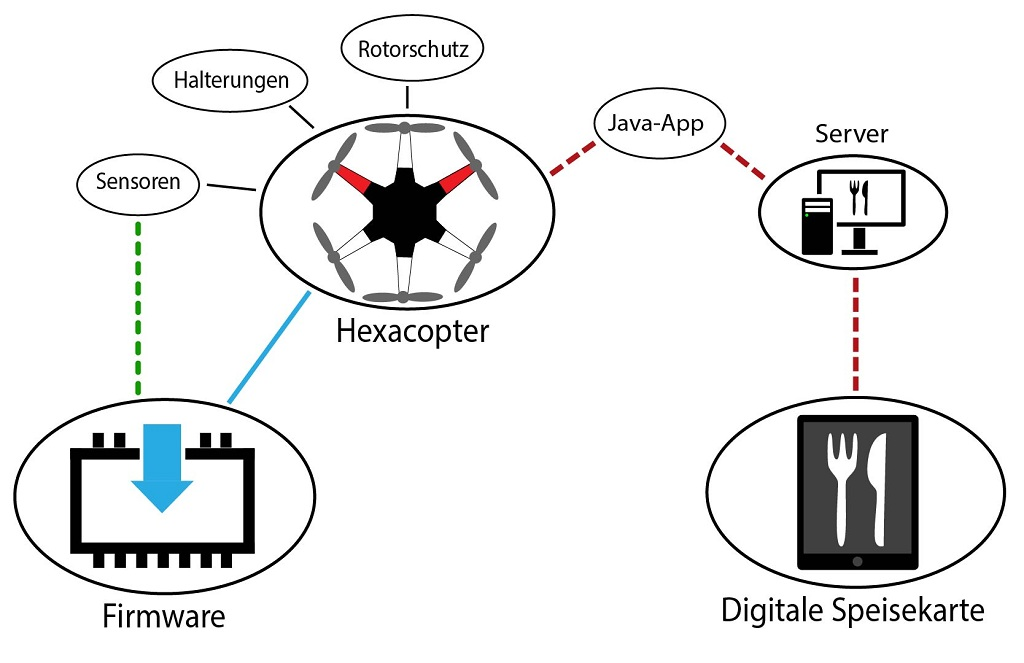
\includegraphics[width = 0.9\textwidth]{Bilder/systemblockbild.jpg}
  \par\end{centering}
  \caption{Systemblockbild}
  \label{Systemblockbild}
\end{figure}

Der Multicopter ist die zentrale Komponente des Projekts. Er ist für den selbstständigen Transport von Objekten zuständig,
und muss somit flugfähig, und im Stande sein Unfälle zu verhindern. Sensoren, die mittels eigens angefertigter Halterungen
am Multicopter befestigt sind, kommunizieren mit der Firmware.

Die Firmware regelt alle logischen Prozesse des Systems. Sowohl die Steuerung des Multicopters, als auch der
Austausch von Daten fällt unter diese Kategorie. Befehle erhält sie unter anderem von der Speisekarte, mit der sie über
einen Server, beziehungsweise einer weiteren Anwendung kommuniziert.

Die digitale Speisekarte ist indirekt die externe Steuereinheit des Multicopters, und zugleich die Komponente,
die das System für den Einsatz in der Gastronomie auszeichnet. Sie automatisiert Vorgänge eines gastronomischen
Betriebs und wandelt Nutzereingaben in Befehle für den Muticopter um.

%%%%%%%%%%%%%%%%%%%%%%%%%%%%%%%%%%%%%%%%%%%%%%%%%%%%%%%%%%%%%%%%%%%%%%%%%%%%%%%
\section{Ausgangssituation}
  In den folgenden Absätzen wird beschrieben, wie die Idee von Hovering Steward, dem autonom fliegenden Kellner
  entstanden ist, und womit sich die ersten Recherchen zu Begin des Projektes beschäftigt, beziehungsweise
  welche Ergebnisse diese hervorgebracht haben.

  \subsection{Ideenfindung}
  Ihren Anfang fand die Idee im Projektmanagement Unterricht. Klasseninterne Teams mussten ein fiktives Projekt erfinden, um auf Basis dieses
  Projektmanagementpläne zu erstellen. Es entstand "Fluorescent Bakery", eine Bäckerei, die fluoreszierende Cupcakes verkauft.
  Der technische Teil ergab sich später, bei dem Gedanken diese Idee für die Diplomarbeit weiterzuverwenden. Der Ansatz hierfür war,
  einen nicht menschlichen Kellner zu erschaffen, der selbstprogrammiert, die Aufgaben einer Bedienung in einem Restaurant übernimmt.
  So entstand "Hovering Steward - der autonom fliegende Kellner", ein dreidimensionales "Tracking-System", welches eine Drohne in einem Raum die Aufgaben eines Kellners durchführen lässt.
  Das Projekt erhielt später noch eine weitere Komponente, nämlich eine digitale Speisekarte, um das automatische System zu erweitern.

  \subsection{Stand der Technik}
  \subsection*{Themenrestaurants}

  \begin{itemize}
    \item \textbf{Disaster Café}

    Das Themenrestaurant {Disaster Café\cite{disastercafe}} in Spanien bietet Gästen die Erfahrung, ihr Essen bei einem Erdbeben
    der Stärke 7.8 zu sich zu nehmen.

    \item \textbf{Das stille Örtchen - Modern Toilet}

    Eingerichtet wie eine Toilette, können Gäste des {Modern Toilet\cite{moderntoilet}} in Japan ihre Speisen in einem gewohnten Umfeld genießen.

    \item \textbf{Affen-Kellner}

    {Eine kleine Taverne in Japan\cite{affenkellner}} besitzt zwei kleine Affen, die Tätigkeiten wie das Servieren von Getränken oder Handtüchern
    für den Inhaber übernehmen. Sie verstehen sogar, welche Getränke ein Gast bestellt.

    \item \textbf{The Royal Dragon}

    Neben Rollschuh fahrenden Kellnern verfügt das weltweit größte {Restaurant für Meeresfrüchte\cite{royaldragon}} eine
    Art Seilbahn, mit der ein Kellner "fliegend" das Essen serviert.

    \item \textbf{Dinner in the Sky}

    Bei {Dinner in the Sky\cite{dinnerinthesky}} werden die Gäste samt Tisch und kleiner Küche von einem Kran 50 Meter
    in die Luft gezogen, wo dann gespeist wird.

    \item \textbf{Dinner in the Dark}

    In diesem {Themenrestaurant\cite{dinnerinthedark}} verbringen die Gäste ihren Aufenthalt im Dunkeln. Einzig und allein die
    Kellner können mittels Nachtsichtbrille etwas sehen.

  \end{itemize}

  \subsection*{Multicopter in der Gastronomie}
  \begin{itemize}
      \item \textbf{Infinium-Serve}

      Das Unternehmen {Infinium-Robotics\cite{infiniumserve}} hat ein System entwickelt, welches Gästen eines Restaurants
      das Essen mittels Hexacopter serviert.

      \item \textbf{iTray}

      {iTray\cite{itray}}, ein Projekt aus London, nutzt kleine Drohnen um Sushi an die Tische der Gäste zu bringen.
      Die Drohnen werden über ein Remote-Wi-Fi-System gesteuert.

  \end{itemize}

  \subsection*{Multicopter Projekte}
  \begin{itemize}
      \item \textbf{ETH Flying Machine Arena}

      Die {"Flying Machine Arena"\cite{eth}} ist ein portables System, welches einen virtuellen Raum mit den Maßen 10x10x10 Meter aufbaut, in welchem
      Objekte mit hoher Präzision erkannt und verfolgt werden können. Das System ist für Experimente mit autonom fliegenden Hexacoptern
      gedacht, die sich in diesem virtuellen Raum über drahtlose Kommunikation orientieren können.

      \item \textbf{Lily}

      {Lily\cite{lily}} ist eine selbstständig fliegende Drohne mit eingebauter Kamera. Ihr Zweck ist, dass sie den Benutzer auf seinem Weg verfolgt.
      Sie wird dafür einfach in die Luft geworfen, worauf sie sich stabilisiert. Danach folgt sie dem Benutzer in einem festgelegten Abstand, solange dieser ein, für Lily
      vorgesehenes Armband trägt und filmt mit einer HD Kamera alles mit.

      \item \textbf{DHL Paketcopter}

      Der {DHL Paketcopter\cite{dhl}} ist ein Innovationsprojekt der DHL, bei dem ein Paket per Drohne zugestellt wird. Die Drohne ist in der Lage große Strecken zu fliegen,
      und somit auch zu schwer erreichbaren Orten zu gelangen, wenn Menschen dazu keine Möglichkeit mehr haben. Auf der Insel Juist wird sie beispielsweise als
      Medikamentenversorger verwendet, da am Wochenende keine Lieferungen per Schiff auf die Insel zugestellt werden.

      \item \textbf{Ambulance Drone}

      Die {Ambulance Drohne\cite{ambulancedrone}} ist ein Projekt, welches auf der TU Delft entwickelt wird. Das Besondere an dieser Drohne ist, dass sie einen eingebauten Defibrillator hat, welcher
      sich per Fernverbindung von einem Rettungshelfer bedienen lässt, obwohl dieser nicht anwesend ist. Die Ambulance Drohne fliegt mit einer Höchstgeschwindigkeit von bis zu
      100 Stundenkilometer und kann somit, in einem Notfall, schnell die Unfallstelle erreichen.

      \item \textbf{Gimball}

      {Gimball\cite{gimball}} ist der weltweit erste fliegende Roboter, der immun gegen Kollistionen ist. Seine Konstruktion besteht aus einem kugelförmigen Gerüst, in dem die Drohne
      aufgehängt ist, und sich anhand von Gelenken trotzdem frei darin bewegen kann. Die Kugel fängt Stöße ab, wodurch die Drohne ungehindert an schwer erreichbare
      Orte gelangt.

  \end{itemize}

%%%%%%%%%%%%%%%%%%%%%%%%%%%%%%%%%%%%%%%%%%%%%%%%%%%%%%%%%%%%%%%%%%%%%%%%%%%%%%%
\section{Team und Aufgabenverteilung}
  \subsection*{Markus Kaiser}
  \textbf{Projektleitung und Marketing}

  Markus Kaiser leitete das Team Hovering Steward und war somit für das Projektmanagement und
  die organisatorischen Aspekte verantwortlich. Neben dieser Hauptrolle zählte außerdem das Marketing
  zu seinen Aufgabenbereichen, was speziell die Entwicklung des Blogs anbelangte. Durch seine Kenntnisse
  in der Webentwicklung stellte er mit dem Blog eine wichtige Schnittstelle zur Außenwelt her.

  \subsection*{Lucas Ullrich}
  \textbf{Sensorik \& Firmware}

  Lucas Ullrich war neben seiner Position als Projektleiter Stellvertreter für die Sensorik an unserer Drohne und
  für die Programmierung der Firmware zuständig. Er unterstützte unseren Projektleiter bei terminlichen Angelegenheiten
  und konnte durch seine Kenntnisse mit der Programmiersprache C eine solide Basis für die Firmware des Microcontrollers schaffen.
  Außerdem entwarf er die Schaltpläne, und erstellte somit ein Konzept für die Sensorik.

  \subsection*{Christina Bornberg}
  \textbf{Firmware}

  Christina Bornberg fungierte als Firmware Entwicklerin des Teams. Durch ihre Interesse an der Programmierung von Drohnen
  und bereits gesammelten Erfahrung mit der Programmierung von C konnte sie gemeinsam mit Lucas Ullrich die erarbeiteten Konzepte hinter
  dem automatisierten Flug der Drohne in Code realisieren.

  \subsection*{Katharina Joksch}
  \textbf{Webentwicklung}

  Der Aufgabenbereich von Katharina Joksch war die Webentwicklung, genauer gesagt die Programmierung der digitalen Speisekarte.
  Neben der Planung der Datenbank und der sinnvollen Verwendung hilfreicher Frameworks entwickelte sie außerdem eine Java Applikation,
  die die Kommunikation zwischen der digitalen Speisekarte und der Drohne regelte.

  \subsection*{Alexander Punz}
  \textbf{Hardware \& Mechanik}

  Alexander Punz war sowohl für die Hardware, als auch für die Mechanik verantwortlich. Seine Aufgaben waren sowohl die Konzeption
  und Produktion des Rotorschutzes, der einen sicheren Flug der Drohne ermöglichte, als auch die Herstellung diverser Halterungen,
  die für Sensorik, Transport und Flugtests verausgesetzt waren.

%%%%%%%%%%%%%%%%%%%%%%%%%%%%%%%%%%%%%%%%%%%%%%%%%%%%%%%%%%%%%%%%%%%%%%%%%%%%%%%
\section{Betreuer}
  \subsection*{Mag. Andreas Fink}
  Mag. Andreas Fink stand dem Projektteam als Hauptbetreuer der Abteilung für Informationstechnologie zur Seite.
  Seine objektive Sichtweise auf das Projekt, hat dem Team sehr geholfen den Fokus auf die Ziele zu legen und
  das Projekt in die Richtung zu entwickeln.
  Zusätzlich dazu betreute er individuell Markus Kaiser bei den Aspekten Projektleitung und Marketing.

  \subsection*{DI Herbert Fleck}
  DI Herbert Fleck war Hauptbetreuer der Mechatronik Abteilung unseres Teams. Er koordinierte den Prozess der Diplomarbeit
  gemeinsam mit Mag. Andreas Fink. Das Team schätzte außerdem sehr das konstruktive Feedback bei Präsentationen.
  Er betreute nebenbei Lucas Ullrich mit Fachwissen aus dem Bereich der Elektronik.

  \subsection*{DI August Hörandl}
  DI August Hörandl fungierte als Individualbetreuer von Christina Bornberg. Duch seine Fähigkeiten und
  Erfahungen als Programmierer sowohl mit der Sprache C, als auch Java war das Entwickeln der Firmware,
  aber auch der Java-Applikation für die WLAN-Kommunikation wesentlich einfacher. Außerdem war
  DI August Hörandl unser Ansprechpartner wenn es Unklarheiten bei \LaTeX gab.

  \subsection*{MMag. Florian Weiss}
  MMag. Florian Weiss betreute Katharina Joksch bei der Entwicklung der digitalen Speisekarte. Sein umfangreiches
  Know-How im Bereich der Webentwicklung, dem Umgang mit diversen Frameworks und Bibliotheken half Katharina
  dabei ein Grundgerüst für die Entwicklung aufzubauen.

  \subsection*{DI Franz Temper}
  DI Franz Temper unterstützte Alexander Punz bei der Entwicklung der Konstruktionen. Durch Fachwissen mit
  der Software Creo und Unterstützung bei 3D-Druck war es möglich, dass Alexander alle seiner Ziele erfolgreich
  umsetzen konnte.

%%%%%%%%%%%%%%%%%%%%%%%%%%%%%%%%%%%%%%%%%%%%%%%%%%%%%%%%%%%%%%%%%%%%%%%%%%%%%%%
\section{Partner / Sponsoren}

\subsection*{GRZ IT Center GmbH}
{GRZ IT Center\cite{grz}} ist eines der größten Rechenzentren österreichs. Mit dem Fokus auf Bankenservicierung arbeitet das Unternehmen
mit Partnern wie Raiffeisen zusammen. Auf eine Anfrage für ein Sponsoring der Diplomarbeit erhielten wir die überaschende
Antwort, dass GRZ das Projekt sehr interessant findet, und uns aus diesen Gründen als Hauptsponsor, mit einem beträchtlichen Betrag
unterstützen würde.
Es wurde ein Sponsoringvertrag, auf Basis einer Mustervorlage aufgesetzt, in welchen beidseitig Konditionen für die Partnerschaft
verfasst wurden, und von beiden Parteien unterzeichnet.

\subsection*{OFI}
{Das Österreichische Forschungsinstitut\cite{ofi}} ist Experte die Prüfung für Werkstoffanwerundung
und Bauwerkserneuerungen. Neben finanzieller Unterstützung erhielt das Projektteam
ein professionelles, projektbegleitendes Team-Coaching, inklusive Zertifikat.

\subsection*{EVOtech GmbH}
Dank der Firma {EVOtech\cite{evotech}} war es möglich additive Module für den Hexacopter selbst anzufertigen.
Das gesamte für den 3D-Druck benötigte Material wurde gesponsert.

\subsection*{LivingPhotos}
{LivingPhotos\cite{livingphotos}} ermöglichte uns, unsere Internetauftritte durch professionelle Teamfotos und Portraits aufzuwerten.


\chapter{Projektmanagement}
\renewcommand{\kapitelautor}{Autor: Markus Kaiser}

%%%%%%%%%%%%%%%%%%%%%%%%%%%%%%%%%%%%%%%%%%%%%%%%%%%%%%%%%%%%%%%%%%%%%%%%%%%%%%%
\section{Ziele}
Im folgenden Abschnitt werden zusammengefasst die Muss-, optionalen und Nicht-Ziele angeführt.
Die Formulierungen sind aus dem Kontext, der Ziele aus dem Projektantrag (vgl. Anhang; Projektmanagement) entnommen, und für die
Zusammenfassung umformuliert worden.

  \subsection{Muss-Ziele}
  \textbf{Zusammenbau des Multicopters}

  Der ausgewählte Multicopter ist soweit zusammengebaut, dass er flugfähig ist.
  Zusätzliche Komponenten, wie Fernbedienung, Akkus und Ersatzteile liegen vor.

  \textbf{Konzeptstudie: Sensorik}

  Um ohne manuelle Einfüsse fliegen zu können und sein Ziel zu finden braucht der Multicopter eine Reihe
  von Sensoren. Diese dienen zur Positions-bzw. zur Objekterfassung. Das Konzept beinhaltet außerdem eine
  Maßnahme für die Kommunikation zwischen Multicopter und Sensoren.
  Der Multicopter ist mit den Sensoren verbunden und bekommt von ihnen die notwendigen Informationen.

  \textbf{Konzeptstudie: Navigation}

  Es existiert ein Konzept, wie der Multicopter die richtige Flugroute zum gewünschten
  Zielort findet. Dazu zählt sowohl der Teil der Firmware, der für den automatisierten Flug programmiert ist,
  als auch die Positionierung anhand von Sensoren und Wegmarkierungen.

  \textbf{Konzeptstudie: Objekterkennung}

  Es liegt ein Konzept vor, wie der Multicopter anhand von Sensoren Hindernisse oder Zielobjekte
  erkennen und diesen ausweichen, oder sie ansteuern kann.

  \textbf{Konzeptstudie: Sicherheit}

  Für den Fall eines Systemausfalls liegt ein Konzept vor, wie der Multicopter sicher landen kann.
  Weiters besteht die Möglichkeit, in den manuellen Flugmodus umzuschalten.

  \textbf{Testen der Konzeptstudien}

  Um festzustellen, ob sich die erarbeiteten Konzepte auch in der Praxis bewähren und sich somit der Einsatz teurer Kameratrackingsysteme rentieren könnte, sind diese umgesetzt.
  Als Sensoren sind eine Kamera sowie Ultraschallsensoren verwendet.

  \textbf{Speisekarte}

  Eine digitale, für ein automatisches Kellnersystem entwickelte Speisekarte läuft auf einem Tablet,
  und bietet Funktionen wie die Auflistung der Speisen, die Bestellung und die Verarbeitung der Bestellung.
  Außerdem gibt es eine Möglichkeit dem Multicopter Informationen zu schicken.

  \textbf{Blog}

  Die Diplomarbeitswebsite fungiert in erster Linie als selbst programmierter Blog, um Interessenten
  jederzeit die Möglichkeit zu bieten, sich über den Status des Projektes zu informieren. Jedes Teammitglied
  kann im Backend-Bereich individuelle Blog- oder Entwicklertagebucheinträge über ein Benutzerkonto verfassen.

  \subsection{Optionale Ziele}
  \textbf{Erweiterte Funktionalitäten der Speisekarte}

  Administratoren haben bestimmte Verwaltungsmöglichkeiten.

  \textbf{Multicopter Erweiterungen}

  Platinen für die Kommunikation zwischen Multicopter und Basis sind angefertigt.
  Sensoren sind mittels Halterungen am Multicopter befestigt.
  Es gibt eine Möglichkeit ein Objekt auf dem Multicopter zu platzieren und es sicher zu transportieren.

  \textbf{Firmware Erweiterungen}

  Der Multicopter empfängt Informationen drahtlos von einem Server,
  wertet diese aus und verarbeitet sie im Anschluss.
  Grundfunktionen wie Steigen, Rollen oder Nicken sind programmiert.

  \subsection{Nicht-Ziele}
  \textbf{Mehrere Multicopter}

  Das System ist fähig, mehrere Multicopter gleichzeitig zu steuern, ohne Abstürze
  zu verursachen oder Menschen zu gefärden.

  \textbf{Sicherheitsmaßnahmen}

  Das Projekt enthält keine Sicherheitsmaßnahmen, die Verletzungen von Menschen
  verhindern und das Risiko eines Absturzes senken.

  \textbf{Erfolgreiche Konzeptstudie}

  Das Ziel der Diplomarbeit ist es, dass das konzeptionierte System zwingend
  funktionsfähig umgesetzt ist.

%%%%%%%%%%%%%%%%%%%%%%%%%%%%%%%%%%%%%%%%%%%%%%%%%%%%%%%%%%%%%%%%%%%%%%%%%%%%%%%
\section{Management-Methode}
Das nachfolgende Kapitel beschäftigt sich mit den wesentlichen Unterschieden
zweier Projektmanagement-Methoden und der Wahl der Methode für diese Diplomarbeit.

  \subsection{Bewährte Methoden}
  \subsection*{Agile Methoden}
  Das Kennzeichen agiler Entwicklungsmethoden wie beispielsweise Scrum oder Kanban, sind
  ein iterativer Arbeitsprozess, Flexibilität, gute und häufige Kommunikation und vorallem
  Selbstständigkeit. Es wird kurz geplant und fortlaufend angepasst. Da nur bedingt eine Reihenfolge
  von zu erledigenden Tasks besteht finden sich diese Methoden oft in der Softwareentwicklung vor.

  \subsection*{Klassische Methoden}
  Klassischen Entwicklungsmethoden zeichnen sich durch eine phasenorientierte Arbeitsweise aus.
  Ganz besonders die Planungsphasen sind sehr umfangreich, um das Risiko später auftretender Probleme oder
  Änderungen zu minimieren. Alle Ziele sind klar definiert und Tasks bis in kleinste Details ausformuliert.

\subsection{Die gewählte Methode}
Für die Entwicklung von Hovering Steward, war eine Kombination beider Methoden notwendig. Da,
das Projekt sich sowohl aus einigen Software-, als auch Hardwarekomponenten zusammensetzt, war das
Ziel sowohl die Vorteile der Flexibilität von agilen Methoden, als auch die ausführliche Planung der klassischen
Methoden auszunutzen.

Es entstand eine Mischung aus der agilen Entwicklungsmethode Scrum und der klassischen Methode Wasserfall.
Für die Entwicklung der Firmware des Multicopters, aber auch die der webtechnologischen Komponenten eignete
sich die flexible Arbeitsweise von Scrum, da nach Bedarf die einzelnen Module der Software entwickelt, und Schritt
für Schritt in das System integriert wurden.
Die Fertigung der Halterungen am Multicopter bedarfen jedoch einer genauen Planung der Reihenfolge von Arbeitsschritten,
welche mithilfe eines Projektstrukturplans visualisiert wurden.

%%%%%%%%%%%%%%%%%%%%%%%%%%%%%%%%%%%%%%%%%%%%%%%%%%%%%%%%%%%%%%%%%%%%%%%%%%%%%%%
\section{Teammanagement / Teambuilding}
Da sich das Team aus sowohl aus Schülern verschiedener Klassen, aber auch Fachrichtungen
zusammensetzte war Teambuilding ein wichtiger Teil des Managements. Das Projekt bestand außerdem
aus Komponenten, die sich technisch gesehen stark voneinader unterschieden, jedoch gut zusammenarbeiten mussten.
Daher war regelmäßige Kommunikation auch eine Voraussetzung.

  \subsection{KaTeCos}
  Eine Form von internen Meetings, die den Grundstein für die Teamdynamik setzten, waren unsere
  sogenannten "Kaffe Team Coachings", kurz KaTeCo. Eine Projektmanegerin unseres Partnerunternehmens ofi
  bot sich als Coach für das Team an. Alle drei Wochen erhielten wird bei diesen Coachings wertvolle Techniken und
  Strategien, sowohl für das Teambuilding, als auch die Umsetzung des Projekts.

  \subsection{Projektkultur}
  In der Planungsphase wurde gemeinsam eine Projektkultur erarbeitet, die folgende Regeln und Pflichten
  für jedes Teammitglied festlegte.
  \begin{itemize}
    \item Wenn eine Deadline voraussichtlich nicht erfüllt werden kann, wird dem gesamten Team so früh wie möglich Bescheid gegeben.
    \item Jedes Teammitglied ist ehrlich und offen gegenüber den anderen Teammitgliedern
    \item Entscheidungen werden nicht nur vom Projektleiter, sondern vom gesamten Team getroffen.
    \item Jedes Teammitglied hat immer Zugriff auf projektinterne Dateien und Informationen.
    \item Wichtige e-Mails sind zuerst vom gesamten Team abzusegnen, bevor sie verschickt werden.
    \item Probleme werden nicht als Hindernis, sondern als Chance gesehen.
  \end{itemize}


% !TEX root = diplomarbeit.tex
\chapter{Marketing}
\renewcommand{\kapitelautor}{Autor: Markus Kaiser}

%%%%%%%%%%%%%%%%%%%%%%%%%%%%%%%%%%%%%%%%%%%%%%%%%%%%%%%%%%%%%%%%%%%%%%%%%%%%%%%
\section{Allgemein}
Im folgenden Kapitel wird beschrieben, mit welchen Mitteln und mit welcher Effektivität
das Projekt Hovering Steward vermarktet wurde. Unter anderem werden diverse Marktanalysen,
aber auch Marketing-Strategien und deren Anwendung erläutert.

  \subsection{Marktanalysen}
    \subsection*{SWOT-Analyse}
    Mithilfe der SWOT-Analyse wird der aktuelle Zustand eines Unternehmens, oder in unserem Fall Projekts, analysiert, um anschließend eine von vier möglichen Strategien
    für den weiteren Verlauf des Unternehmens zu erarbeiten. Es werden Stärken, Schwächen, Möglichkeiten und Risiken evaluiert, wobei sich jeweils Stärken und Schwächen, und
    Chancen und Gefahren gegenüberstehen. Die vier Begriffe, auf englisch übersetzt \textbf{S}trengths, \textbf{W}eaknesses, \textbf{O}pportunities und \textbf{T}hreats,
    ergeben dadurch das Akronym SWOT.

    \begin{figure}[H]
      \begin{centering}
      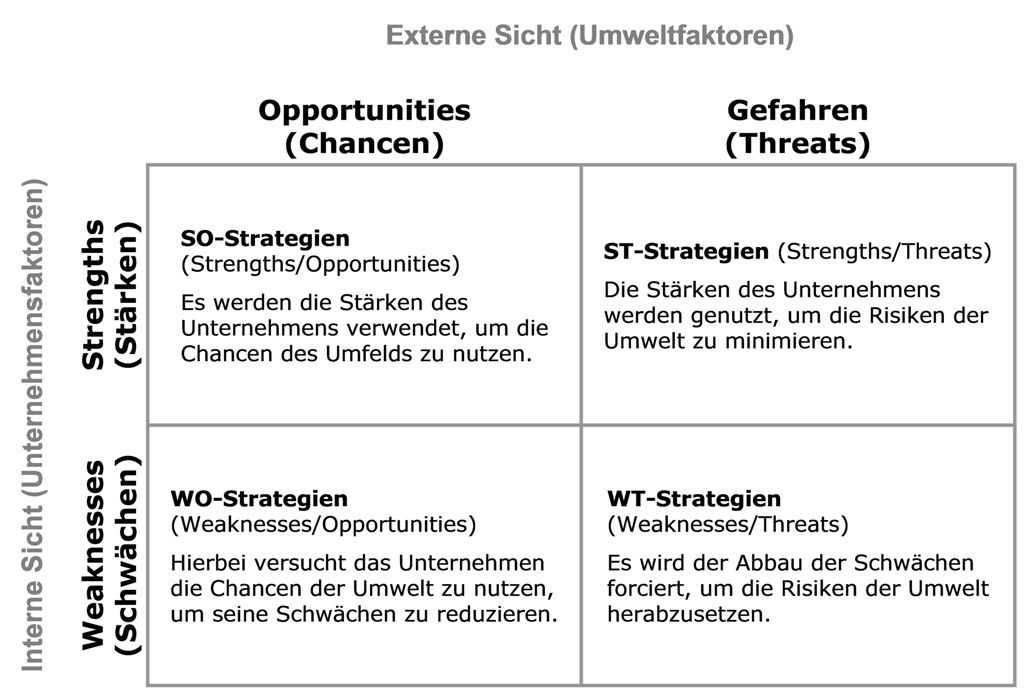
\includegraphics[width = 1\textwidth]{Bilder/swot.jpg}
      \par\end{centering}
      \caption[SWOT-Analyse]{SWOT-Analyse\cite{pic_swot}}
      \label{swot}
    \end{figure}

    \subsection*{Die vier Strategien:}
    \begin{itemize}
      \item \textbf{SO-Strategie}

      Die Stärken des Unternehmens werden hervorgehoben und mit den Chancen verknüpft. Macht ein Unternehmen beispielsweise hohe Umsätze in Industrieländern und hat
      genügend finanzielle Mittel, wird expandiert und ein neuer Standort in einem weiteren Industrieland aufgebaut.

      \item \textbf{ST-Strategie}

      Auch hier werden die Stärken des Unternehmens genutzt, allerdings um bestehende Gefahren einzuschränken oder zu entfernen. Besteht die Gefahr, dass die Konkurrenz
      einen höheren Marktanteil erlangt, kann das Unternehmen beispielsweise durch eine sehr gute Marketingabteilung neue Produkte planen, die dies verhindern.

      \item \textbf{WO-Strategie}

      Hierbei wird versucht, die Schwächen eines Unternehmens als Chance zu sehen, sich weiterzuentwickeln. Erzielt ein gewisses Produkt nicht die erwarteten Gewinne,
      können durch neue Lösungsansätze neue Erfahrungen gewonnen werden, die nach Erfolg auch auf andere Produkte angewendet werden können.

      \newpage

      \item \textbf{WT-Strategie}

      Die Schwächen des Unternehmens werden näher betrachtet, um beim Versuch diese zu dezimieren, gleichzeitig Gefahren einzugrenzen. Diese Strategie kann sehr hilfreich
      sein, wenn das Unternehmen sich auf dem Markt schwer über Wasser halten kann.
    \end{itemize}

    \subsection*{Portfolioanalyse nach Boston Consulting Group}
    Die Definition laut {Boston Consulting Group\cite{portfolioanalyse}} beschreibt die Portfolioanalyse wie folgt:
    "Das BCG-Portfolio erlaubt eine Bewertung strategisch relevanter Geschäftseinheiten auf Basis zukünftiger Gewinnchancen (Marktwachstum) und der
    gegenwärtigen Wettbewerbsposition (relativer Marktanteil)."
    Anders gesagt: Diese Analyse hilft dabei Teile eines Unternehmens wie Produkte oder Dienstleistungen
    nach Kosten und Ertrag einzuschätzen und in vier Kategorien zu unterteilen.

    \begin{figure}[H]
      \begin{centering}
      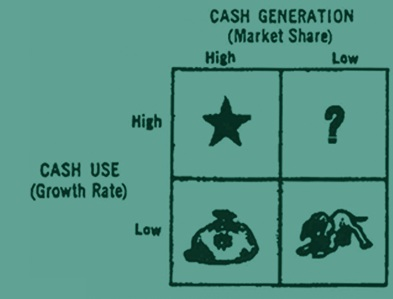
\includegraphics[width = 1\textwidth]{Bilder/portfoliomatrix.jpg}
      \par\end{centering}
      \caption[Portfoliomatrix]{Portfoliomatrix\cite{pic_matrix}}
      \label{matrix}
    \end{figure}

    \begin{itemize}
      \item Die \textbf{Cashcow} ist ein Produkt des Unternehmens, welches sich bereits lange Zeit auf dem Markt hält und dadurch hohe Gewinne erziehlt. Durch die
      erarbeitete hohe Position auf dem Markt decken sich ihre Kosten durch den Gewinn selbst. Die Cashcow stellt zudem die Basis für die Weiterentwicklung anderer
      Produkte dar.

      \item Der \textbf{Superstar} ist ein Produkt mit den besten Aussichten. Es erzielt bereits nach kurzer Zeit auf dem Markt hohe Gewinne. Um den Marktanteil
      zu halten, muss jedoch viel in dieses Produkt investiert werden. In der Regel geschieht dies durch die Überschüsse, die die Cashcow abwirft.

      \item Ein \textbf{Poor Dog} ist ein weniger erfolgreiches Produkt. Da es nach hohen Investitionen und langer Zeit auf dem Markt keine nennenswerte
      Gewinne erbracht hat, ist es ratsam zu überlegen, ob weiter investiert, oder die Produktion gestoppt wird.

      \item Als \textbf{Questionmarks} werden die Produkte bezeichnet, bei denen sich noch nicht eindeutig gezeigt hat, in welche Richtung sie sich entwickeln werden.
      Es steht offen, ob sie zu einem Superstar oder einem Poor Dog werden. Diese Tatsache macht es schwer zu entscheiden, ob weiter in sie investiert, oder das Produkt
      verkauft wird.
    \end{itemize}

    \subsection*{SWOT-Analyse von Hovering Steward}
    Da sich die Portfolioanalyse nach der Boston Consulting Group eher für Unternehmen eignet, die mehrere Produkte oder Dienstleistungen anbieten, war sie für das Projekt
    Hovering Steward weniger relevant. Aus diesem Grund wurde eine SWOT-Analyse durchgeführt.

    \begin{figure}[H]
      \begin{centering}
      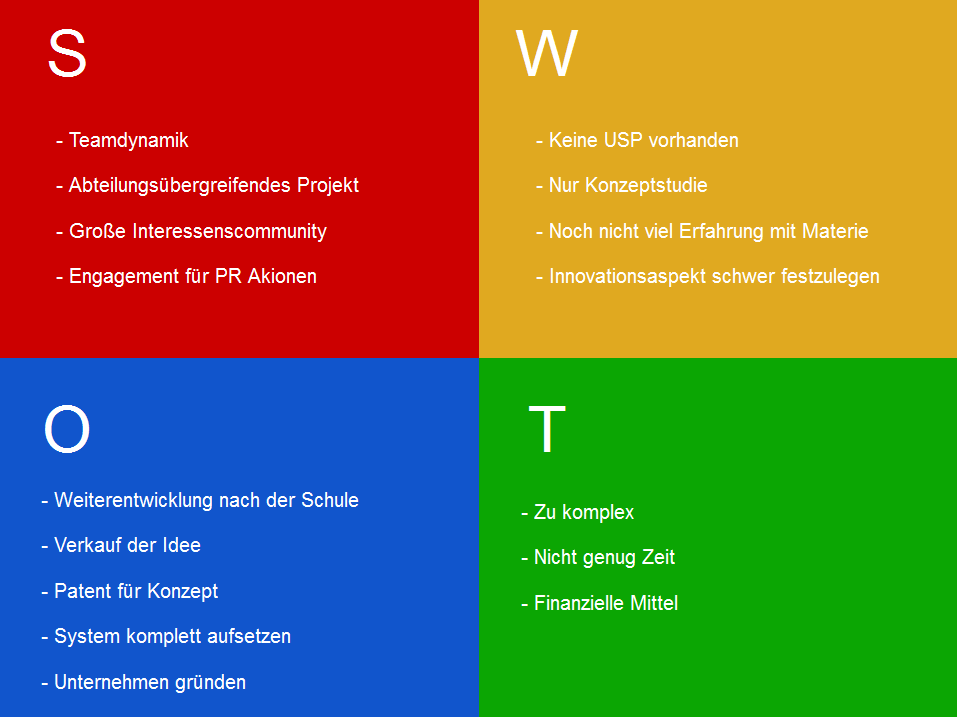
\includegraphics[width = 1\textwidth]{Bilder/hovi_SWOT.png}
      \par\end{centering}
      \caption{SWOT-Analyse von Hovering Steward}
      \label{hoviswot}
    \end{figure}

  \subsection{Marketing-Strategie}
  Aus der SWOT-Analyse ging hervor, dass die Schwächen des Projekts großteils darin lagen, es nur schwer präsentieren zu können, da das Hauptziel das Entwickeln
  einer Konzeptstudie, keines fertigen Produktes ist. Außerdem ergaben Kostenabschätzungen, dass das Testen der Konzepte einen hohen finanziellen Aufwand mit sich bringen
  würde. Aus diesen beiden Erkenntnissen entstand das Vorhaben, das Projekt sehr aktiv an die Öffentlichkeit zu bringen. Es sollten zum einen Fortschritte im Projekt
  für Außenstehende ersichtlich gestaltet werden und zum anderen Kontakt mit potentiellen Sponsoren und Partnern hergestellt werden, um folglich das Budget des Projekts
  zu decken. Diese Vorgehensweise fällt unter die Kategorie der WT-Strategie, auf Basis der SWOT-Analyse.

    \subsection*{Corporate Design}
    Um einen professionellen Eindruck bei Internetauftritten und Events zu vermitteln, wurde ein Corporate Design entwickelt.
    Das Corporate Design diente als Guideline für das Gestalten jeglicher visueller Verweise auf die Diplomarbeit Hovering Steward.
    Es wurden Eigenschaften für das Logo, bestimmte Farben und zu verwendende Fonts festgelegt.
    Somit war es möglich dem Projekt ein einheitliches Auftreten in der Öffentlichkeit, und damit einen Wiedererkennungswert zu verleihen.

    \subsection*{Visitenkarten}
    Um die Außenwelt auf unser Projekt aufmerksam zu machen, wurden Visitenkarten entworfen, die sich von anderen Projekten abheben.
    Sie sollten sowohl die notwendige Information auf den ersten Blick vermitteln, als auch ein anspruchsvolles Design repräsentieren. Aus dem Vorhaben,
    mit Marketing Transparenz in unserem Projekt zu schaffen, entstand die Idee, die Karten zum Teil transparent zu gestalten.
    Das Ergebnis war folgendes:

    \begin{figure}[H]
      \begin{centering}
      
\includegraphics[width = 1\textwidth]{Bilder/visitenkarte.jpg}
      \par\end{centering}
      \caption{Visitenkarte von Hovering Steward}
      \label{visitenkarte}
    \end{figure}

    \subsection*{Blog}
    Der Blog war die wichtigste Komponente für das Veröffentlichen von akuellen Informationen. Es wurde Wert darauf gelegt
    in regelmäßgen Abständen aktuelle Inhalte über den Projektverlauf zu veröffentlichen. Die Zielgruppe waren primär junge Techniker,
    die sich für Drohnen oder allgemein für Robotik interessierten. Alles zur Entwicklung des Blogs ist in Kapitel 3.3 angeführt.
    Durch sämtliche folgende Punkte wurde versucht, die Zielgruppe auf den Blog aufmerksam zu machen.

    \subsection*{Wettbewerbe}
    Hovering Steward hat an einigen Wettbewerben teilgenommen, auf welche im Kapitel 3.2 näher eingegangen wird.
    Folgende Erwartungen waren eine Motivation, eine Bewerbung für diese einzuschicken:

    \begin{itemize}
      \item \textbf{Teamdynamik}

      Bei einer Präsentation vor fremdem Publikum war ein professionelles Auftreten, gute Planung und vorallem Koordination gefragt.
      Diese Auftritte wurden sowohl als Chancen genutzt, die Dynamik im Team weiterzuentwickeln, als auch Präsentationstechniken für
      die Endpräsentation zu trainieren.

      \item \textbf{Unterstützung}

      Ein weiterer Vorteil war, dass durch die Teilnahme an Wettbewerben von den veranstaltenden Unternehmen, Unterstützung geboten wurde. Nicht nur im finanziellen
      Bereich, sondern auch durch Workshops oder ähnliche hilfreiche Events.

      \item \textbf{Marketing}

      Nicht zuletzt waren Wettbewerbe ein wichtiger Teil des Marketings, da sich die Projektidee nicht nur durch Präsentationen verbreiten ließ,
      sondern auch in den zozialen Medien und auf den Webseiten der Veranstalter erwähnt wurde.

    \end{itemize}


%%%%%%%%%%%%%%%%%%%%%%%%%%%%%%%%%%%%%%%%%%%%%%%%%%%%%%%%%%%%%%%%%%%%%%%%%%%%%%%
\section{Public Relations}

  \subsection{Wettbewerbe, Events & Präsentationen}

    \subsection*{Jugend Innovativ}
    {Jugend Innovativ\cite{jugendinnovativ}} ist einer der bekanntesten Bewerbe, die Schul- und Diplomarbeitsprojekte
    unterstützen. Wie der Name schon sagt, legt die Jury hierbei sehr großen Wert auf den innovativen
    Aspekt der Projektidee. Zu diesem Zweck wurde eine umfangreiche Executive Summary verfasst, die nicht
    nur auf den technischen Hintergründen basiert, sondern hervorhebt, was das Projekt einzigartig
    macht. Das Team hat das Halbfinale von Jugend Innovativ erreicht, und somit eine finanzielle Unterstützung
    zugesagt bekommen.

    \subsection*{Bosch - Technik fürs Leben Preis}
    Die Bosch-Gruppe Österreich ist Initiator des jährlichen Wettbewerbs {"Technik fürs Leben"\cite{bosch}}. Es werden Österreichs
    größte Talente des technisch orientierten Nachwuchses gesucht. Projekte werden von einer Experten-Jury bewertet,
    der Hauptpreis is das Angebot für ein Praktikum bei der Bosch-Gruppe Österreich.

    \subsection*{Accenture HTL Challenge}
    Der Managementberatungs-, Technologie- und Outsourcing Dienstleister {Accenture\cite{accenture}} veranstaltet jedes Jahr die Accenture HTL Challenge,
    bei der Projekte und Diplomarbeiten von technischen Schulen, rund um das Thema Informationstechnologie gesucht werden.
    Die Teams treten durch Präsentationen vor einer Jury gegeneinander an. Neben dem Wettbewerb werden den Teilnehmern außerdem
    Unterstützungen wie Coachings und Beratungen von Experten angeboten. Aufgrund des Umfangs dieses Wettbewerbs wurden die erforderlichen Bewerbungsunterlagen eingesendet,
    um das Projekt auch hier an die Öffentlichkeit zu bringen, und bei Gelegenheit Kontakte zu knüpfen. Hovering Steward schaffte es ins Finale der
    Accenture HTL Challenge.

    \subsection*{ITs Project Award}
    Der {ITs Project Award\cite{its}} ist ein Event der FH Salzburg. Projekte und Diplomarbeiten aus den Bereichen Informations- und Kommunikationstechnologie
    können eingereicht werden, aufsteigende Teams treten in einem Finale gegeneinander an und müssen ihr Projekt präsentieren. Bewertet werden die
    Teams von einer Experten-Jury nach Kriterien wie Kreativität, Innovationsaspekt oder wirtschaftlicher Relevanz.
    Auch in diesem Bewerb erreichte Hovering Steward das Finale.

    \subsection*{Invasion der Drohnen}
    Zu Begin der Diplomarbeit wurde versucht, möglichst viel über die Entwicklung und den Einsatz von Drohnen zu erfahren.
    Der Vortrag {Invasion der Drohnen\cite{invasionderdrohnen}}, mit anschließender Diskussion zum Thema "Entwicklung von Drohnen, Einsatzgebiete und rechtliche Einschränkungen" brachte
    viele neue Informationen, wie der Umgang mit unbemannten Flugobjekten, speziell in Österreich gehandhabt wird.

    \subsection*{European Conference on Educational Robotics}
    Über den Wettbewerb Accenture wurde Kontakt mit dem Leiter der {European Conference on Educational Robotics\cite{ecer}} hergestellt.
    "Die European Conference on Educational Robotics (ECER) ist eine internationale, wissenschaftliche Konferenz für Schüler. Wissenschaftler
    geben mit Vorträgen Einblick in ihre Forschung, führen Roboter live vor und sind Punkterichter bei spannenden Robotikbewerben.
    Teilnehmende Teams präsentieren ihre Roboter, Projekte und Erfahrungen nach wissenschaftlichem
    Vorbild in englischer Sprache."
    Von unserem Auftritt und unserer Idee überzeugt, wurden wir von dem Leiter der ECER eingeladen, unser Projekt zu präsentieren.

    \subsection*{{Maturaprojekt-Wettbewerb FH Kärnten\cite{fhkaernten}}}
    Auch bei diesem Wettbewerb reichen Maturaprojekt-Teams aus ganz Österreich ihre Projektideen ein.
    Mit einer Teilnehmerzahl von knapp 120 Projekten ist der Wettbewerb einer der größten Österreichs. Eine
    Experten-Jury aus verschiedenen Fachbereichen wählen sechzehn Teams, die in die engere Auswahl kommen.
    Hovering Steward wurde aus einer Gruppe von 70 Mitstreitern für die Teilnahme am Finale gewählt und konnte somit
    auch an der FH Kärnten das Projekt an die Öffentlichkeit bringen.

%%%%%%%%%%%%%%%%%%%%%%%%%%%%%%%%%%%%%%%%%%%%%%%%%%%%%%%%%%%%%%%%%%%%%%%%%%%%%%%
\section{Blog}
Dieses Kapitel setzt sich mit dem Entwicklungsprozess der technischer Planung, bis zur Implementierung
des Blogs, auseinander. Es werden technische Hintergründe, wie verwendete Technologien, aber
auch allgemeine Überlegungen wie der Einsatz eines Content Management Systems, behandelt.

  \subsection{Technische Planung}
  Der folgende Abschnitt umfasst alles, von den ersten Gedanken der technischen Planung, sowie der Umsetzung,
  des, für das Projekt programmierten Blogs.

    \subsection*{Überlegungen}
    Es stellte sich bereits früh im Projekt heraus, dass die Fertigstellung eines komplexen Vorhabens wie diesem, nicht in
    dem Zeitrahmen der Diplomarbeit durchführbar ist. Dadurch, dass ein Großteil der Ziele daraus besteht, Konzepte für die
    einzelnen Komponenten zu entwickeln, blieb wenig Zeit diese auch zu testen. Es gab also nur sehr beschränkt die Möglichkeit,
    den Fortschritt der Diplomarbeit vorzuzeigen, beispielsweise indem der Hexacopter bereits selbstständig eine Route fliegt.
    Dazu kam, dass bezüglich des Flugrechts von unbemannten Luftfahrzegen in Österreich, keine konkreten Bestimmungen, was das Fliegen einer Drohne in einem
    geschlossenen, öffentlichen Raum betrifft, aufzufinden waren.

    Um Interessenten trotzdem Transparenz über den Fortschritt und Entwicklungsmethoden in unserem Projekt zu bieten, wurde
    die Entwicklung eines Blogs geplant, indem die Teammitglieder selbstständig, von Zeit zu Zeit Arbeitsschritte, als auch
    Ergebnisse veröffentlichen konnten.

    \subsection*{Content Management Systeme}
    Der Blog fungiert als \textbf{C}ontent \textbf{M}anagement \textbf{S}ystem, kurz CMS. Der Zweck eines
    Content Management Systems ist der, dass duch Trennung von Inhalt und Design eine
    sehr einfache Nutzung ermöglicht wird. Gewöhnliche Nutzer müssen keine besonderen
    Kenntnisse über das Bearbeiten oder Erstellen einer Website vorweisen, sondern
    können über einfache Eingabefelder Text, Bilder oder Videos auf einer Website einbinden.

    Zu den meist genutzten Content Management Systemen am Markt zählen unter anderem die Open-Source-CMS {TYPO3\cite{typo3}},
    {Wordpress\cite{wordpress}} oder {Drupal\cite{drupal}}. Der Grund, warum keines dieser Content Management Systeme für die
    Entwicklung des Blogs gewählt wurde, ist in Kapitel 3.3.5 vermerkt.

    \subsection*{Mockups}
    Die Überlegungen bezüglich des Designs des Blogs unterschieden sich stark zwischen den ersten
    Entwürfen und der schlussendlich gewählten Variante.

    Die Wahl der Farben basierte ursprünglich auf einer Studie der deutschen Schriftstellerin Eva Heller,
    die mit ihrem Buch {"Wie Farben wirken"\cite{WieFarbenWirken}} analysierte, welche Farbtöne von einem Großteil der Menschen
    mit welcher Eigenschaft verbunden werden. Der Fokus von Hovering Steward lag darin, die zwei Begriffe "Hunger"
    und "Appetit" möglichst gut zu vermitteln. Das Resultat war eine Kombination der Farben Braun, Gelb und Rosa, die mit diesen beiden Begriffen
    assoziiert wurden. Den Blog mithilfe dieser Farbkombination zu gestalten, erschien jedoch nicht passend, weswegen
    ein zweiter Ansatz notwendig war.

    Die Überlegung, den Blog gleich wie die digitale Speisekarte zu gestalten, führte dazu, Elemente, die an ein Restaurant
    erinnern, einzubinden. Dies führte zu der Idee, einen Holztisch im Hintergrund abzubilden.
    Damit das Design trotzdem einen modernen Eindruck macht, wurde für die Darstellung von Inhalten ein {"Flat Design"\cite{FlatDesign}}
    herangezogen. Das Flat Design zeichnet sich vor allem durch sehr vereinfache Gestaltung, grelle Farben und zweidimensionale Abbildungen aus.
    Es ist auf optimale Usability, also verständliche und einfache Nutzung, ausgelegt.

    Das Endresultat war folgendes:

    \begin{figure}[H]
      \begin{centering}
      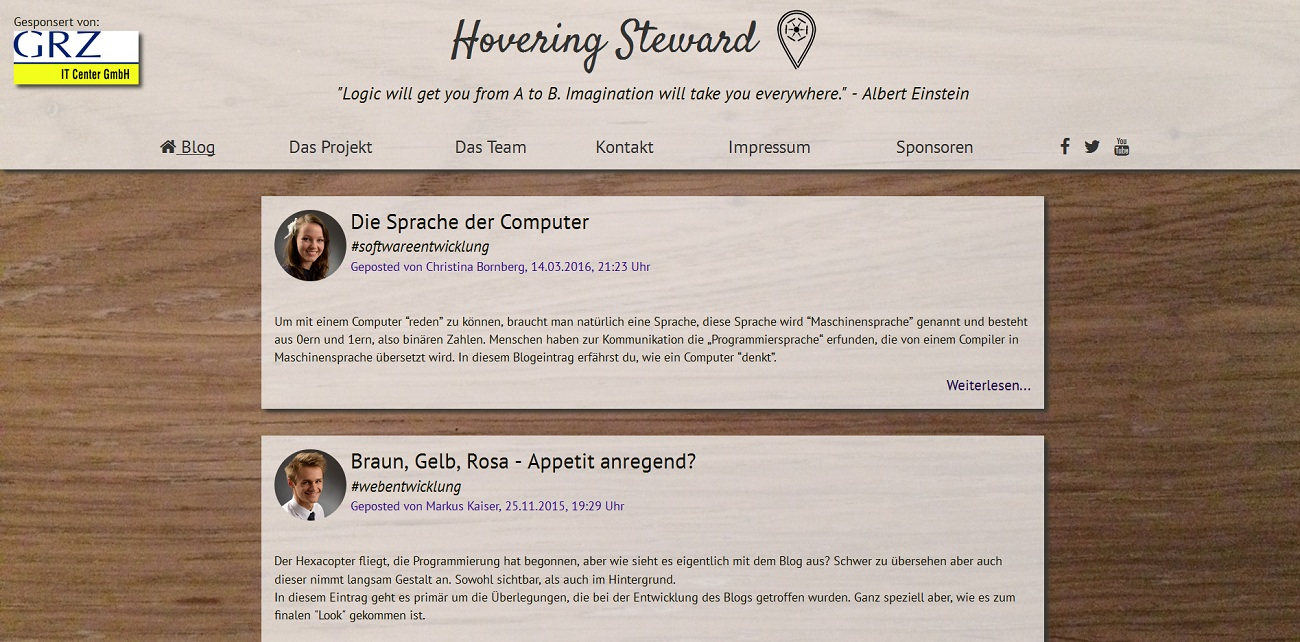
\includegraphics[width = 1\textwidth]{Bilder/blog_dashboard.jpg}
      \par\end{centering}
      \caption{Dashboard des Blogs von Hovering Steward}
      \label{blog}
    \end{figure}

    \subsection*{Frameworks}
    Für die Entwicklung des Blogs erschien der Einsatz eines Frameworks als sehr hilfreich. Das Framework sollte komplexe Methoden wie
    Datenbankzugriffe oder Formularvalidierungen vereinfacht zur Verfügung stellen. Für bessere Übersicht während der Entwicklung war es außerdem
    wichtig, dass das Framework auf dem MVC-Schema(vgl. Kapitel 4.2.1) aufbaut. Dieses Schema wird in Kapitel 4.2.1 erklärt. Eine Recherche ergab folgende Frameworks als mögliche
    Optionen:

    \begin{itemize}
      \item Laravel
      \item Symfony
      \item CodeIgniter
      \item CakePHP
    \end{itemize}

    Die Wahl fiel auf CodeIgniter, die Begründung dafür ist in Kapitel 3.3.5 angeführt.

  \subsection{Umsetzung}

    \subsection*{Frontend}
    Das Frontend des Blogs setzt sich aus den drei Technologien HTML, Javascript und CSS zusammen. Aus Gründen von Performance und SEO(vgl. Kapitel 3.3.2) wurden außerdem
    die Javascript Bibliothek jQuery und das CSS Framework Bootstrap verwendet. Im Folgenden werden diese Technologien näher beschrieben und die daraus
    ersichtlichen Vorteile, die zu Verwendung in diesem Projekt geführt haben, erläutert.

      \subsubsection*{HTML}
      Die {\textbf{H}yper \textbf{T}ext \textbf{M}arkup \textbf{L}anguage\cite{html}} ist eine gängige Auszeichnungssprache die dazu verwendet wird, Dokumente mit Text und Medien zu strukturieren.
      Ein HTML-Dokument ist das Grundgerüst einer Website. Ein Webbrowser interpretiert
      HTML und visualisiert dadurch die Website. Die Syntax von HTML besteht aus sogenannten Tags, die, nach einem
      bestimmten Schema aufgebaut, die Struktur einer Website ergeben. Die aktuelle Version ist HTML 5. Diese unterstützt zum einen das responsive
      Entwickeln einer Website, und verbessert zum anderen die SEO. Außerdem ist es möglich ohne eines Plugins wie des Adobe Flash Players Audio und Video einzubinden.

      \subsubsection*{Javascript}
      {Javascript\cite{javascript}} ist eine webbasierende Skriptsprache. Sie ist objektorientiert, was bedeutet, dass modular programmiert werden kann und damit Funktionen oder Eigenschaften
      durch Vererbung einmal geschrieben und mehrmals wiederverwendet werden können. Die Sprache wird genutzt, um eine Website dynamisch mittels Vorgängen wie Berechnungen oder Animationen auf einer Website durchzuführen.
      Oft sind diese mit Interaktion des Nutzers verbunden. Javascript greift hierfür auf das Document Object Model des HTML-Dokumtens zu, um Elemente und Knoten in diesem hinzuzufügen, zu löschen oder
      zu ändern. Ein großer Vorteil von Javascript ist, dass durch das Einbinden von auf Javascript basierenden Bibliotheken, ganz leicht eine Vielzahl von zusätzlichen Funktionen
      verwendet werden können.

      Javascript ist nachwievor die am weitesten verbreitetste Skriptsprache für Webanwendungen, die am Client verarbeitet wird. Sie wird stark unterstützt, wodurch auch einfach Hilfestellungen im Netz
      gefunden werden können. Es gab daher keinen Grund, eine Alternative zu Javascript in Betracht zu ziehen.

      Ein gutes Beispiel, und zugleich auch eine, für den Blog verwendete Bibliothek ist {jQuery\cite{jquery}}.
      jQuery ist eine Open-Source Javascript Bibliothek, mit dessen Entwicklung versucht wurde, die Nachteile von Javascript zu beheben. Einer der wesentlichen Vorteile ist
      der vereinfachte Zugriff und die Manipulation von DOM-Elementen.

      Beispiel Javascript:

\lstset{language= html }
\begin{lstlisting}
/**
* Liefert alle <li> Elemente, die sich in einem Element
* mit der ID "navbar-list" befinden.
**/
var list = document.getElementById("navbar-list");
var items = list.querySelectorAll("li");
\end{lstlisting}

\newpage

      Beispiel: jQuery:

\lstset{ language=html }
\begin{lstlisting}
/**
* Liefert alle <li> Elemente, die sich in einem Element
* mit der ID "navbar-list" befinden.
**/
var items = $("#navbar-list li");
\end{lstlisting}

      Ein derzeit sehr aktuelles Javascript Framework ist {AngularJS\cite{angular}}. Die Intention dieses Frameworks ist die Automatisierung von oft verwendeten Vorgängen durch
      Datenbindungen und Direktiven. Der Programmierer erspart sich dadurch Codezeilen und Zeit. Zu den sinnvollen Einsatzgebieten von Angular zählen Webseiten mit großteils dynamisch generiertem
      Inhalt oder auch "Single Page Applikations", Webseiten, die einmal geladen werden und dann nur zwischen Inhalten wechseln, ohne diese neu zu laden. Das Framework in Kombination mit dem PHP
      Framework CodeIgniter zu verwenden bedeutete jedoch eine flache Lernkurve. Der Blog war zudem nicht als "Single Page Applikation" geplant, wodurch sich die Verwendung von AngularJS nicht rentiert hätte.

      \subsubsection*{CSS}
      {CSS\cite{css}} steht für \textbf{C}ascading \textbf{S}tyle \textbf{S}heets. Wie das Wort "Style" bereits offenbart, wird sie für das visuelle Aufbereiten einer Website verwendet.
      Allgemein ist CSS eine Gestaltungssprache und wird in Kombination mit HTML-Dokumenten verwendet. In HTML werden dafür den Tags Klassen oder IDs
      zugewiesen, über die CSS dann bestimmte Eigenschaften zuweisen kann. Dabei orientiert sich CSS an dem sogenannten Box-Modell. In diesem werden HTML-Elemente
      zwischen Inline-Elementen und Block-Elemente unterschieden. Inline-Elemente passen sich dem Fluss in der Struktur des Dokuments an, Block-Elemente hingegen
      werden für das Layout der Website verwendet. Von einfachen Formatierungen wie der Schriftgröße oder einer Hintergrundfarbe lassen sich mit CSS komplexe Animationen,
      ohne die Verwendung von Javascript durchführen. Letzteres ist jedoch erst seit der Version CSS3 möglich.

      Das Open-Source Framework {Twitter Bootstrap\cite{bootstrap}} gilt eigentlich als CSS-Framework, da den Elementen die Eigenschaften über CSS Klassen zugewiesen werden, es basiert jedoch
      ebenfalls auf HTML und Javascriptcript. Neben dem wesentlichen Vorteil der responsiven Gestaltung einer Website, bietet es durch
      zahlreiche, vordefinierte Javascript Methoden, die ebenfalls durch die Zuweiseung von Klassen an Elemente gebunden werden, die Möglichkeiten, animierte Dropdown-Menüs, Pop-Up-Windows oder Bildergalerien einzubinden.
      Weitere wichtige Eigenschaften von Bootstrap sind die weitreichende Browserkompatibilität und das einheitliche Design.

      Eine Alternative zu Bootstrap stellt {Foundation\cite{foundation}} dar. Es ist ebenso wie Bootstrap ein CSS Framework, mit dem ein responsives Gestalten einer Website umsetzbar ist.
      Da das Framework einen sehr ähnlichen Umfang aufwies, fiel die Wahl jedoch auf Bootstrap, da damit bereits öfters gearbeitet wurde und somit weniger Zeitaufwand bedeutete.

    \subsection*{Backend}
    Das Backend baut ausschließlich auf dem Framework CodeIgniter auf, welches auf der serverseitigen Scriptsprache PHP basiert. Für die Datenspeicherung
    wurde eine MySQL-Datenbank verwendet.

      \subsubsection*{Code}
        \subsubsection*{PHP}
        {PHP\cite{php}, ausgeschrieben \textbf{P}HP \textbf{H}ypertext \textbf{P}reprocessor, ist genau wie Javascript eine Skriptsprache, mit dem Unterschied, dass der Code nicht auf dem Client, sondern auf dem Server ausgeführt wird
        und im Anschluss für den Client lesbares HTML generiert. Dies bietet den großen Vorteil, dass für den Client nicht ersichtlich ist, was im Hintergrund an PHP Code ausgeführt
        wird. Um PHP zu programmieren, wird allerdings ein Webserver mit einer PHP-Installation benötigt.

        \subsubsection*{Ruby}
        {Ruby\cite{ruby}} ist eine Alternative zu PHP. Neben dem Einsatz in der Webentwicklung wird diese Skriptsprache allerdings auch für allgemeinere Softwareentwicklungsgebiete verwendet.
        Für die Webentwicklung stellt Ruby das Framework {"Ruby on Rails"\cite{rubyonrails}} zur Verfügung.
        Da Ruby jedoch noch keinen so hohen Bekanntheitsgrad wie PHP hat, gibt es weniger ausführlichere Dokumentationen, weswegen PHP als die sinnvollere Variante für das Backend des Blogs erschien.
        Außerdem ist die Überlegung, eine Website in Ruby zu entwickeln damit verbunden, einen geeigneten Webhoster zu finden, welcher über eine Ruby Installation auf dem Server verfügt.

        \subsubsection*{Perl}
        {Perl\cite{perl}} ist, ähnlich wie Ruby, eine Skriptsprache für vielseitige Nutzung, wie Systemadministration, Netzwerkprogrammierung, aber auch Webentwicklung, was sie
        zu einer weiteren Alternative zu PHP macht. Neben dem Vorteil der Plattformunabhängigkeit ist Perl mit den Sprachen HTML und MySQL kompatibel. Beide dieser Sprachen stellen
        einen wichtigen Bestandteil des Blogs dar. Da Perl jedoch im Vergleich zu PHP nicht ausschließlich für die Entwicklung von Webanwendungen vorgesehen ist, sind
        Methodenaufrufe oft viel komplexer, was einen höheren Aufwand bei der Programmierung bedeutet hätte.

      \subsubsection*{Datenbank}

        \subsubsection*{MySQL}
        MySQL ist ein weit verbreitetes relationales Datenbanksystem, das auf SQL basiert. SQL steht für "Structured Query Language" und bezeichnet eine Datenbanksprache.
        Sie wird verwendet, um die Struktur einer Datenbank festzulegen, Daten hinzuzufügen, diese zu ändern oder zu löschen. MySQL stellt eine wichtige Schnittstelle zwischen zwei gängigen Sprachen für
        die Entwicklung dynamischer Webseiten zu Verfügung, indem sie es ermöglicht, diese Abfragen mit der Scriptsprache PHP durchzuführen. Ein hilfreiches Verwaltungstool ist phpMyAdmin,
        eine in PHP entwickelte Anwendung, die die Verwaltung der MySQL Datenbanken über eine grafische Oberfläche vereinfacht.

        \subsubsection*{MongoDB}
        Anders als MySQL, ist {MongoDB\cite{mongodb}} eine NoSQL Datenbank. Der Unterschied liegt darin, dass die Datenbank nicht relational ist. Statt eines konkreten Schemas von Tabellen,
        wird hier mit sogenannten Dokumenten und Sammlungen gearbeitet. Ein Dokument speichert Daten, nach dem "Key-Value" Prinzip, eine Sammlung enthält mehrere Dokumente.
        Den bedeutendsten Vorteil weist MongoDB in der dynamischen Gestaltung der Datenbank auf. Die Strukturen in Sammlungen können demnach unterschiedlich sein. Die
        Datenübermittlung erfolgt über {BSON\cite{bson}}, ein JSON ähnliches Format, welches im Vergleich zu diesem jedoch auch Datentypen unterstützt.

        Eine Verbindung zu MongoDB über CodeIgniter aufzubauen erwies sich als Nachteil, da zu diesem Zweck eigene Bibliotheken, für beispielsweise das Arbeiten mit Sessions,
        einzubinden gewesen wären.

    \subsection*{SEO}
    Der Blog war unsere wichtigste Schnittstelle nach Außen, weswegen er im Internet leicht zu finden sein musste. Suchmaschinen wie Google oder Bing nutzen
    sogenannte Robots, kleine Programme, die selbstständig das World Wide Web durchstöbern, um Webseiten zu inspizieren und zu bewerten. Je besser die Bewertung,
    desto weiter oben lässt sich die Website in der Suchmaschine auffinden.
    Die Bewertung hängt von einer Vielzahl von Kriterien ab, von denen folgende bei der Entwicklung des Blogs beachtet wurden:

    \begin{itemize}
      \item \textbf{Aufbau der Seite}

        Die Grundstruktur eines HTML Dokuments besteht aus den drei Teilen:

        \begin{itemize}
          \item Dokumenttyp-Dekleration
          \item head
          \item body
        \end{itemize}

        und sieht wie folgt aus:

\lstset{language = html}
\begin{lstlisting}
<!DOCTYPE html>
<html lang="de">
  <head>
    <meta charset="utf-8">
    <meta name="viewport" content="width=device-width,initial-scale=1.0">
    <title>Titel</title>
  </head>
  <body>
  </body>
</html>
\end{lstlisting}

        Ganz oben im Dokument wird der Dokumenttyp deklariert. Dieser gibt die verwendete HTML Version an. Im Falle von HTML 5 würde dieser wie folgt aussehen:

\lstset{language = html}
\begin{lstlisting}
<!DOCTYPE html>
\end{lstlisting}

        Der Dokumenttyp für HTML 4.01 Strict hingegen wurde wie folgt angegeben:

\lstset{language = html}
\begin{lstlisting}
<!DOCTYPE HTML PUBLIC "-//W3C//DTD HTML 4.01//EN"
"http://www.w3.org/TR/html4/strict.dtd">
\end{lstlisting}

        Im \textless head \textgreater Bereich werden \textless meta \textgreater Tags angegeben, in denen allgemeine und technische Informationen zur Website, wie Zeichensatz
        und Skalierung bei mobiler Version, oder Keywords und Beschreibung gespeichert werden.
        Die beiden Letzten sind besonders wichtig, da sie dem Robot mitteilen, worum es auf der Seite geht. Er achtet hierbei auch darauf, dass die Beschreibung nicht
        länger als 155 Zeichen lang ist und die Keywords eindeutig gewählt werden.

        Im \textless body \textgreater, also im eigentlichen Inhalt der Website legt der Robot zum einen sehr viel Wert auf Struktur. Beispielsweise muss die Verschachtelung der Tags stimmen,
        oder der \textless h1 \textgreater Tag darf nur einmal pro Seite vorkommen.
        Zum anderen werden Inhalt und Code in Relation gesetzt. Wenn der Aufbau des HTML Dokuments sehr groß ist, in jedem Absatz jedoch nur ein Satz steht, kennt sich der Robot nicht aus.

      \item \textbf{Responsive Design}

        Das Smartphone ist mittlerweile ein ebenso beliebtes Gerät zum Surfen im Internet, wie der Desktop PC. Damit auf dem kleinen Display alles gut lesbar ist, muss die Website speziell
        gestaltet werden. Frameworks, wie Bootsrap, helfen bei diesem Vorhaben, indem mithilfe von vordefinierten CSS-Klassen die Elemente der Website so gestaltet werden, dass diese mit der
        Bildschirmgröße mitwachsen, sich verschieben oder ausgeblendet werden.

      \item \textbf{Interne und externe Links}

        Bei Links werden sowohl Links, die auf die Website verweisen, als auch Links, die auf andere Seiten zeigen bewertet.
        Zeigen sehr viele externe Links auf eine Seite, interpretiert der Robot diese als geläufig und sie erhält eine höhere Wertung. In unserem Fall war die Kombination mit anderen sozialen
        Medien sehr hilfreich, da durch Veröffentlichungen auf diesen automatisch Links auf den Blog generiert werden.

        Links, die von der eigenen Seite auf andere verweisen stellen jedoch einen Nachteil dar, da der Robot dem Link folgen könnte, statt die eigene Seite weiter zu inspizieren. Möchte man dies
        verhindern, kann dem \textless a \textgreater Tag das Attribut rel="nofollow" hinzugefügt werden, um dem Robot zu sagen, dass er diesem Link nicht folgen soll.

      \item \textbf{Sitemap}

      	Die Sitemap ist ein Inhaltsverzeichnis der Website, z.B. in Form einer XML Datei. Die Sitemap hilft dem Robot, wenn er erst einmal auf einer Seite gelandet ist, zugehörige Seiten
        zu finden. Dadurch, dass in der Sitemap die zugehörigen Unterseiten einer Seite mittels URL angegeben werden, hat dies den selben Vorteil wie eine große Anzahl externer Links, die auf diese
        Unterseiten verweisen, nämlich dass Google diese schneller findet. Tools wie xml-sitemaps.com bieten an, eine Sitemap für die angegebene URL zu generieren. Hat der Robot die Seite vollständig
        untersucht, muss die Sitemap im Domain Root-Verzeichnis abgelegt werden. Zuletzt kann die URL zu dieser Sitemap bei Google registriert werden, um Google anzuweisen einen Robot über die Seite
        laufen zu lassen. Nach einigen Tagen sind die Ergebnisse direkt in der Google Suche sichtbar.

      \item \textbf{Browserkompatibilität}

        Nicht jeder Browser stellt jede Seite gleich dar. Die Tags werden unterschiedlich, oder sogar gar nicht verstanden. Wird dies nicht beachtet, wirkt sich das auf die Nutzerfreundlichkeit
        und damit auch auf die Bewertung der Website aus. Um dies zu verhindern, gibt es Tools wie zum Beispiel {caniuse.com\cite{caniuse}}, in denen genau verzeichnet ist, welcher Tag oder welche CSS-Eigenschaft
        von welchem Browser, beziehungsweise welcher Browserversion unterstützt wird.

      \item \textbf{Ladezeit}

        Der Robot bewertet ebenfalls die Ladezeit einer Website. Sie ergibt sich aus der Anzahl an Bildern, Videos oder eingebundenen Bibliotheken oder Schriftarten auf der Website.
        Speziell beim Blog war früh klar, dass viele Bilder geladen werden müssen. Den Upload auf eine niedrige Dateigröße einzuschränken hat zu Beginn nicht ausgereicht.
        Eine Javascript Bibliothek names {YoxView\cite{yoxview}} hat es allerdings ermöglicht, die Bilder erst dann zu laden, wenn ein Nutzer auf einen Thumbnail klickt. Die Größe der Thumbnails betrugen bloß
        ein paar Kilobyte, wodurch die Ladezeit der Website bedeutend verkürzt werden konnte.

    \end{itemize}

  \subsection{Implementierung}

    \subsection*{FTP Client}
    Für die Verwaltung der Website wurde der Open-Source FTP-Client {FileZilla\cite{filezilla}} verwendet. Ein Nutzer kann eine Verbindung zu einem FTP-/SFTP
    Server herstellen und folglich Verzeichnisse und Dateien auf diesem Server hoch- und herunterladen. {FTP\cite{ftp}} steht für File Transfer Protocol. Es ermöglicht
    den bidirektionalen Austausch von Dateien zwischen Endgeräten. {SFTP\cite{sftp}} bedeutet Secure File Transfer Protocol, nutzt das SSH Protokoll und bietet somit
    einen sichereren Datenaustausch als FTP, da hierbei keine Daten in Klartext, sondern verschlüsselt übertragen werden.

    In Relation zur Notwendigkeit, unsere Dateien zu verschlüsseln, waren die Kosten eines SFTP-Servers jedoch zu hoch, weswegen wir uns für einen einfachen FTP Server entschieden haben.

  \subsection{Herausforderungen und Lösungen}

    \subsection*{Sicherheit}
    Zwei der größten Sicherheitslücken bei Webanwendungen sind zum einen {"Cross-Site-Scripting"\cite{xss}} und zum anderen {"SQL-Injections"\cite{sqlinjections}}.

      \subsubsection*{Cross-Site-Scripting}
      Unter Cross-Site-Scripting, kurz genannt XSS versteht man die Injizierung von schadhaftem Code in eine Webapplikation, über eine Schnittstelle, zu der ein Nutzer
      einfachen Zugang hat. In den meisten Fällen geschieht dies, wenn ein Nutzer gezielt Javascript Code über ein Formular auf einer Website in die Anwedung schleust.
      Gelangt dieses Script an einen anderen Enduser, kann es dort beispielsweise ungehindert auf Cookies zugreifen, da der Browser des anderen Endusers nicht weiß,
      dass dem Script nicht zu vertrauen ist.

      Der Beste Weg XSS zu unterbinden ist, die Eingaben, die über ein Formular vom Nutzer an den Server gesendet werden über PHP zu validieren und notfalls Zeichen, die
      XSS andeuten, zu ersetzen. PHP stellt dafür die Methode htmlspecialchars() zur Verfügung. Sie konvertiert bestimmte Sonderzeichen in HTML-Code. Beispielsweise wird
      das Zeichen \textless , welches notwendig ist um Javascript mittels \textless script \textgreater-Tag zu schreiben, durch "\&lt;" ersetzt.

      \subsubsection*{SQL-Injections}
      Bei einer SQL-Injection hingegen injiziert ein Nutzer SQL-Statements in eine Anwedungung, um somit Daten aus der Datenbank auszulesen, oder diese zu manipulieren.
      Wird SQL Code dynamisch und mittels Nutzer Eingaben generiert, kann der Nutzer diese Statements manipulieren. Werden über ein Formular
      geschickte Daten per "\$\_POST['name'];" direkt in ein SQL Statement übernommen, ohne auf korrekte Zeicheneingabe, Länge des Strings oder Ähnliches validiert wird,
      können Fehler entstehen, die Schaden an der Datenbank anrichten.

      Eine Möglichkeit eine SQL Injection zu verhindern ist, ähnlich wie bei XSS, bestimmte Zeichen zu erkennen und stattdessen als Strings weiterzuverwenden.
      Mit einem einfachen Hochkomma ist es möglich einen Wert zu unterbrechen und an dieser Stelle SQL-Code einzufügen, die die Abfrage beeinflussen.
      Mit der PHP Methode mysql\_real\_escape\_string() wird vor jedes Zeichen, wie zum Beispiel ein ', ein \textbackslash geschrieben, womit dieses zu einem ganz normalen
      String Ausdruck wird und damit ungefährlich ist.

    \subsection*{Responsive Design}
    Für die responsive Gestaltung des Blogs wurde zwar das Framework Bootstrap, aufgrund des soliden Grid-Layouts, herangezogen, da der Aufbau der Website jedoch aus eigener Hand
    entstanden ist und kein Template verwendet wurde, musste für vollständige Kompatibilität auf mobilen Geräten manuell mit CSS gearbeitet werden.
    Mittels Media-Queries lassen sich CSS-Eigenschaften so definieren, dass sie ab gewissen Bildschirmgrößen aktiv werden. Für die Bildschirmbreiten 1200, 992, 767 und 480
    Pixel wurden verschiedene CSS-Eigenschaften definiert. Diese vier Größen sind von Bootstrap hergeleitet und teilen Geräte in die vier Typen Phones, Tablets,
    Desktop und Large Desktop.

  \subsection{Persönliche Erfahrungen}
    \subsection*{Eigenes CMS}
    Durch die Verwendung der Content Management Systeme TYPO3 und Wordpress im Unterricht, war ich bereits mit diesem Themengebiet vertraut. Was mich speziell interessiert hat war,
    was hinter einem CMS steckt. Ich wollte die Abläufe und verschiedenen Schritte kennen lernen und habe mich aus diesem Grund entschieden, den Blog als eigenes Content Management System
    zu entwickeln. Aus zeitlichen Gründen sollte es allerdings nur die Funktionen einer Nutzerverwaltung und einer Beitragveröffentlichung unterstützen.

    \subsection*{Wahl des Frameworks}
    Die Recherche ergab, dass mehrere, unterschiedlich umfangreiche PHP Frameworks für den Blog geeignet wären. Da nicht genug Zeit war jedes testweise zu installieren und
    sich mit den Grundlagen auseinanderzusetzen, habe ich mich an Rezensionen von Nutzern dieser Frameworks orientiert. CodeIgniter stellte sich als optimales Framework für
    die Entwicklung einer Webanwendung dieser Größe heraus. Es bietet zahlreiche Bibliotheken, die über sehr simple Einbindung die Funktionalitäten erweitern. Meiner Meinung nach war das
    Framework außerdem syntaktisch leichter erlernbar als PHP ansich. Eine Installation war auch nicht notwendig. Die Ordnerstruktur musste nach dem Download nur
    exportiert, und in einem Projektordner von XAMPP(vgl. Kapitel 4.2.1) eingefügt werden. Der Vorbereitungsprozess war dadurch, und dank einer besonders guten Dokumentation, minimal.


% !TEX root = diplomarbeit.tex
\chapter{Digitale Speisekarte}
\renewcommand{\kapitelautor}{Autor: Katharina Joksch}

%%%%%%%%%%%%%%%%%%%%%%%%%%%%%%%%%%%%%%%%%%%%%%%%%%%%%%%%%%%%%%%%%%%%%%%%%%%%%%%
\section{Allgemeine technische Planung}

  \subsection{Entwicklungsumgebungen}

    \subsubsection{PhpStorm}
    
    PhpStorm ist eine integrierte Entwicklungsumgebung für die Programmiersprache PHP, für welche man eine kostenpflichtige Lizenz zur Verwendung benötigt. Diese Entwicklungsumgebung wurde von JetBrains entwickelt und erschien erstmals 2009 auf dem Markt. Zu den besonderen Features von PhpStorm zählen Tools zur Kontrolle der Versionierung, Refaktorisierung, Code- und Syntax-Highlighting. Außerdem unterstützt es PHP-Unit, welches von Symfony verwendet wird und zum Testen von PHP-Skripten dient. 

    \subsubsection{Allgemeiner Code-Aufbau}

	Die Webapplikation baut auf mehreren Komponenten auf, um eine optimale Performance zu gewährleisten. Sie baten neben optionalen Funktionalitäten wie Packabes und Plugins vor allem auch eine strukturierte Arbeitsumgebung.
	In der anschließenden Grafik ist ist der allgemeine Aufbau der Webapplikation abgebildet. Die Hauptkomponente bildet das PHP-Framework Symfony, welches alle weiteren Engines miteinander verknüpft. In der Modelebene wurde mit dem Framework Doctrine und dem Datenbanksystem MySQL gearbeitet. In der View-Schicht kamen der Package Manager Bower, das CSS Framework Bootstrap 4 alpha, die Stylesheet-Sprache Sass, der TaskRunner Gulp, Ajax, jQuery, DOM und die Template Engine Twig zum Einsatz. Der Controller wurde auf der Basis von PHP programmiert. All diese Bibliotheken und Frameworks werden in den dazugehörigen Kapiteln genauer erläutert.
	(Skizze folgt noch)

%%%%%%%%%%%%%%%%%%%%%%%%%%%%%%%%%%%%%%%%%%%%%%%%%%%%%%%%%%%%%%%%%%%%%%%%%%%%%%%
\section{Backend}

  \subsection{Technische Planung}

    \subsubsection{MySQL}

	MySQL ist ein relationales Datenbanksystem, welches sowohl als kommerzielle Enterpriseversion wie auch als Open-Source-Software verfügbar ist. MySQL basiert wie der Name bereits vermuten lässt auf der Datenbanksprache SQL(=Structured Quere Language), welche zur Definition von Datenstrukturen und zum Verwalten von darauf basierenden Datenbeständen zuständig ist. Es dient daher zur elektronischen Datenverwaltung und beruht auf einem tabellenbasierten Datenbankmodell.

    \subsubsection{Apache HTTP Server}

	Der Apache HTTP Server ist eine Open-Source-Software, welche von der Apache Software Foundation entwickelt wurde. Der Apache Webserver kann mit den Betriebsystemen Linux, Unix, Windows, Mac OS X, Betware und OpenBSD arbeiten.

    \subsubsection{MAMP}

	MAMP ist eine Distribution von LAMP, welches auf Linux-Basis entwickelt wurde. Es dient dazu dynamische Webseiten zur Verfügung zu stellen. MAMP ist auf das Betriebssystem Mac OS X angepasst. Das Package verwendet den Apache HTTP Server und das Datenbanksystem MySQL. Außerdem basieren sie auf der Programmiersprache PHP. Dadurch ergibt sich auch die Bezeichnung dieses Softwarepackets, da es sich aus den Anfangsbuchstaben der verwendeten Komponenten zusammenstellt.

    \subsubsection{Doctrine}

	Doctrine ist ein Framework, welches dabei hilft ein objektrelationales Abbild zu erschaffen. Bei objektrelationalen Abbildungen werden Tabellen wie Klassen und Tabellenzeilen wie Objekte behandelt. Das vereinfacht den Zugriff auf verschiedene Datenbanken im Vergleich zu dem Zugriff mittels Plain PHP um ein Vielfaches.

    \subsubsection{Symfony}

	Da Frameworks, welche auf dem Model-View-Controller Schema beruhen, den Arbeitsaufwand erleichtern und dafür sorgen, dass während dem Programmieren eine ordentliche Struktur im Code beibehalten wird, wurde eines als Grundgerüst für die Entwicklung der Applikation verwendet. Nachdem eine Speisekarte viele Informationen enthält, welche in einer Datenbank verwaltet werden sollten, wurde ein PHP-Framework gewählt, welches den Zugriff darauf objektrelational regelt.
	Symfony ist ein Open Source Web Application Framework, welches sowohl das Model-View-Controller Schema nützt als auch den Datenbankzugriff mittels einem objektrelationalen Abbild regelt, weshalb es die ideale Wahl für die Umsetzung der digitalen Speisekarte und des Adminbereichs ist. Wie bereits erwähnt, ergibt sich durch die Einteilung in Model, View und Controller während dem Entwicklungsprozess eine strukturierte Ordnung im Code. In der Model Schicht, welche die darzustellenden Daten zur Verfügung stellt, empfiehlt es sich in der Kombination mit Symfony Doctrine zu verwenden. Die View-Ebene ist für die visuelle Darstellung der Applikation zuständig. Für die  Darstellung werden meistens Templates miteinbezogen. Symfony unterstützt hierbei die Template Engine Twig auf welche im Kapitel „Frontend“ noch genauer eingegangen wird.
	Der Controller verwaltet die Darstellung der Applikation und nimmt von ihr Benutzeraktionen entgegen, wertet diese aus und behandelt sie entsprechend. Außerdem fungiert der Controller als Schnittstelle zwischen Model und View, was bedeutet, dass er die Daten von der einen Schicht zur anderen weiterleitet.

    \subsubsection{ER-Modell}

	Bevor die Datenbank mithilfe von Doctrine generiert wurde, wurde ein Entity Relationship Modell angefertigt um zu visualisieren wie die Tabellenverbindungen am geeignetsten aufbereitet werden können.
	(Bild von ERM folgt noch)

  \subsection{Umsetzung}

    \subsubsection{Framework einrichten}

	Um mit Symfony arbeiten zu können wurde zuerst der Symfony-Installer installiert. Bei einem Gerät mit dem Betriebsystem Mac OS X wurde dies durch die Eingabe folgender Befehle in den Terminal bewerkstelligt:
	\lstset{language = bash}
  	\begin{lstlisting}
	sudo curl -LsS http://symfony.com/installer -o /usr/local/bin/symfony
	sudo chmod a+x /usr/local/bin/symfony
  	\end{lstlisting}

	Anschließend wurde ein Projekt angelegt. Dafür wurde in das Zielverzeichnis gewechselt. Um das Projekt im Anschluss über den Apache Server aufrufen zu können, empfiehlt es sich das Projekt direkt im „htdocs“-Ordner der jeweiligen LAMP Distribution abzuspeichern. Damit das Projekt auf einem Mac OS X basierenden Gerät angelegt wurde, musste der anschließende Befehl in den Terminal eingegeben werden:
	\lstset{language = bash}
  	\begin{lstlisting}
	symfony new PROJEKTNAME lts
  	\end{lstlisting}
	Der Befehl „lts“ legt fest, dass die neueste Version von Symfony verwendet wird.

    \subsubsection{Seitenabrufbarkeit}

	Um Seiten anzulegen, welche später im Browser angezeigt werden konnten, musste man im Controller folgende Schritte erledigen. Zuerst empfahl es sich Action Funktionen anzulegen. Diese wurden passend zu der jeweiligen Seite beziehungsweise zu den dementsprechenden Funktionalitäten benannt, welche im Anschluss angezeigt und ausgeführt wurden. Wenn auf der auszugebenden Seite mit einer Template Engine gearbeitet wurde, wurde als Rückgabewert der Methode der anschließende Code definiert:
	\lstset{language = html}
  	\begin{lstlisting}
	$this->render(`DATEIBEZEICHNUNG.html.twig')
  	\end{lstlisting}
	Die Funktion render() formt den Inhalt des Templates in einen Ausgabewert um, damit die Seite  ausgegeben werden kann.
	Um die Route der Seiten selbst bestimmen zu können, wurde über der Action-Funktion eine Annotation hinzugefügt. Diese wurde folgendermaßen angegeben:
	\lstset{language = html}
  	\begin{lstlisting}
	/**
	* @Route("/ROUTE, name=„ROUTENBEZEICHNUNG“)
	*/
  	\end{lstlisting}
	Damit die erstellte Seite anschließend mit MAMP im Browser aufgerufen werden konnte, musste man einfach den folgenden Link in der Adresszeile eingeben:
	http://IP-ADRESSE:PORT/PROJEKTNAME/web/ROUTE

    \subsubsection{Datenbankgenerierung}

	Für die Generierung der Datenbank wurde die Variante „Code First“ verwendet, da diese die Möglichkeit bietet, im Nachhinein ohne großen Aufwand die Datenbank zu ändern.
	Um die Datenbankeinträge zu erstellen, wurde zu Beginn eine PHP-Datei erstellt in welcher die Tabellen als Klassen und die Tabellenzeilen als Objekte angelegt wurden. Die Variablen wurden allesamt mit dem Zugriffsmodifikator „protected“ deklariert, damit nur Klassen, welche von dieser PHP-Datei erben, auf sie zugreifen können. Anschließend wurde oben in der Datei ein USE-Statement eingefügt, welches definiert, dass die Abkürzung „ORM“ in darauf folgender Verwendung besagt, dass es sich um die Generierung eines objektrelationalen Abbilds handelt.
	\lstset{language = html}
  	\begin{lstlisting}
	use Doctrine\ORM\Mapping as ORM;
  	\end{lstlisting}
	Statt dem Kürzel „ORM“ hätte auch ein beliebiges anderes Wort eingesetzt werden können, auf welches später zugegriffen werden könnte, allerdings ist diese Bezeichnung sehr zu empfehlen, da sie etwaige Verwirrungen vermeidet.
	Um die Klassen später als Tabellen generieren lassen zu können, wurden Annotationen mit folgendem Schema darüber geschrieben:
	\lstset{language = html}
  	\begin{lstlisting}
	/**
 	* @ORM\Entity
 	* @ORM\Table(name=„ TABELLENNAME")
	*/
	class TABELLENNAME
	{
	…
	}
    \end{lstlisting}
	Damit die relationale Datenbank Objekte den richtigen Datentypen zuordnen konnte, wurden diese ebenfalls mit einer Anmerkung versehen. Da es bei Objekten zu unterscheiden gilt ob es sich um einen Primärschlüssel oder Fremdschlüssel handelt als auch ob es ein Texteintrag, Ganzzahleneintrag, Eintrag mit Kommastellen, Booleaneintrag oder gar ein Zeitstempel ist, gibt es hierbei verschiedene Varianten.
	Um eine ID als Primare Key zu definieren wurde folgende Annotation verwendet:
	\lstset{language = html}
  	\begin{lstlisting}
  	/**
     * @ORM\Column(type="integer")
     * @ORM\Id
     * @ORM\GeneratedValue(strategy="AUTO")
     */
  	\end{lstlisting}
	Die erste Zeile legt den Datentyp als Ganzzahl fest und die zweite Zeile sagt aus, dass es sich um den Primärschlüssel handelt. Mit der letzten Zeile wird dafür gesorgt, dass der Wert automatisch generiert wird, sobald eine neue Tabellenzeile erstellt wird.
	Bei einem Eintrag mit Kommazahlen musste der Spaltentyp einfach nur auf „float“ eingestellt werden. Für einen Booleaneintrag wurde zwar als Anmerkung der Typ „boolean“ definiert, jedoch ändert das Datenbanksystem MySQL diese Annotation automatisch in das Datenformat „tinyint“.
	Um einen Texteintrag zu definieren musste sowohl der Datentyp als auch die Länge definiert werden:
	\lstset{language = html}
  	\begin{lstlisting}
  	/**
     * @ORM\Column(type="string", length=ANZAHL_DER_ZEICHEN)
     */
  	\end{lstlisting}
	Damit man einen Zeitstempel erstellen kann, was vor allem für die Bestellungen und die Dokumentation des Datenaustausches mit dem Hexacopter wichtig war, musste die folgende Anmerkung hinzugefügt werden:
	\lstset{language = html}
  	\begin{lstlisting}
  	public function __construct()
    /** @ORM\Column(type="datetime", nullable=false ) */
    protected $zeitstempel;
  	\end{lstlisting}
	Mithilfe von „nullable=false“ wurde festgelegt, dass der Zeitstempel niemals ein null-Wert sein darf.
	Um das Datum generieren zu können, musste eine Konstruktorfunktion dafür geschrieben werden:
	\lstset{language = html}
  	\begin{lstlisting}
  	public function __construct()
    {
        $this->zeitstempel = new \DateTime();

    }
  	\end{lstlisting}
	Damit eine ManyToOne beziehungsweise eine OneToMany Verbindung erstellt werden konnte, musste dies ebenfalls mithilfe von Anmerkungen festgelegt werden.
	Auf der ManyToOne Seite sieht die Annotation dafür folgendermaßen aus:
	\lstset{language = html}
  	\begin{lstlisting}
  	/**
     * @ORM\ManyToOne(targetEntity=„NAME_DER_ZIELTABELLE“, inversedBy=„NAME_DER_AKTUELLEN_TABELLE“)
     * @ORM\JoinColumn(name=„BEZEICHNUNG_DES_FREMDSCHLÜSSELS“, referencedColumnName=„ID_DER_ZIELTABELLE“)
     **/
  	\end{lstlisting}
	In der oberen Zeile musste angegeben werden, zwischen welchen Tabellen die Verbindung geschaffen werden soll. Als Zieleintrag gibt man hierbei die Bezeichnung der Tabelle auf der Seite der OneToMany Verbindung an und als Kehrwerteintrag den Namen der Tabelle, welche der anderen Seite viele Einträge zur Verfügung stellt.
	Um die andere Seite der Verbindung zu generieren, wurde folgende Anmerkung verwendet:
	\lstset{language = html}
  	\begin{lstlisting}
  	/**
     * @ORM\OneToMany(targetEntity="NAME_DER_ZIELTABELLE", mappedBy="NAME_DER_AKTUELLEN_TABELLE")
     **/
  	\end{lstlisting}
	Hierbei mussten nur die Namen der Tabellen angegeben werden, welche miteinander verbunden werden sollen. Damit die vielen Einträge, welche von der anderen Tabelle auf die aktuelle verweisen, musste dafür eine ArrayCollection konstruiert werden:
	\lstset{language = html}
  	\begin{lstlisting}
  	public function __construct() {
        $this->speiseeintraege = new ArrayCollection();
    }
  	\end{lstlisting}
	Damit im Anschluss im Controller auf die Daten zugegriffen werden konnte, musste zu jedem Objekt eine Getter- und eine Setter- Methode erstellt werden. Diese konnte man sich ganz einfach mit einem Rechtsklick über die Menüpunkte „Generate…“ und „Getters and Setters…“ automatisch erstellen lassen.
	Damit der Code aus dieser PHP-Datei in der MySQL Datenbank der LAMP Distribution verwendet werden konnte, musste zuerst eine Datenbank über das PHPMyAdmin-Interface erstellt werden. Darauf folgend musste in der „config.yml“-Datei, welche automatisch in der Symfony Dateistruktur vorliegt, folgendes festgelegt sein:
	\lstset{language = html}
  	\begin{lstlisting}
  	imports:
    - { resource: parameters.yml }
	…
	doctrine:
   	 	dbal:
        	driver:   pdo_mysql
        	host:     "%database_host%"
        	port:     "%database_port%"
        	dbname:   "%database_name%"
        	user:     "%database_user%"
        	password: "%database_password%"
        	unix_socket: /Applications/MAMP/tmp/mysql/mysql.sock
        	charset:  UTF8
	orm:
        	auto_generate_proxy_classes: "%kernel.debug%"
        	naming_strategy: doctrine.orm.naming_strategy.underscore
      	  	auto_mapping: true
  	\end{lstlisting}
	Alle Werte welche mit Anführungszeichen und Prozentzeichen versehen wurden, mussten in der „parameter.yml“-Datei mit Werten deklariert werden:
	\lstset{language = html}
  	\begin{lstlisting}
  	parameters:
    	database_host: IP-ADRESSE
    	database_port: DATENBANKPORT
    	database_name: DATENBANKNAME
    	database_user: USERNAME
    	database_password: PASSWORT
    	mailer_transport: smtp
    	mailer_host: IP-ADRESSE
    	mailer_user: USERNAME
    	mailer_password: PASSWORT
    	secret: GEHEIMCODE
  	\end{lstlisting}
	Mit diesen zwei Dateien wird der Zugriff auf die MySQL Datenbank geregelt.
	Anschließend konnte bereits über den Terminal die Datenbank mit den Tabellen, welche zuvor in der PHP-Datei generiert wurden, in MySQL erstellt werden:
	\lstset{language = bash}
  	\begin{lstlisting}
	php app/console doctrine:generate:entities AppBundle
  	\end{lstlisting}
	Um Änderungen in der Datenbank von der PHP-Datei zu übernehmen, musste anschließend nur noch folgender Befehl in die Konsole eingegeben werden:
	\lstset{language = bash}
  	\begin{lstlisting}
	php app/console doctrine:schema:update —force
  	\end{lstlisting}
	Mit diesen Schritten wurde die Datenbank erfolgreich generiert.

    \subsubsection{Datenzugriff}

	Damit im Controller auf die Einträge der Datenbank zugegriffen werden konnte, musste ein Repository erstellt werden:
	\lstset{language = html}
  	\begin{lstlisting}
  	$repository = $this->getDoctrine()
            ->getRepository(‚AppBundle:TABELLENNAME');
  	\end{lstlisting}
	Mithilfe der Befehle „findAll()“, „findAllByTABELLENSPALTE(WERT“ und „findOneByTABELLENSPALTE(WERT)“ konnten die benötigten Werte aufgerufen werden.
	Diese Werte konnten anschließend, einfach in der render-funktion, welche die auszugebende Seite generiert, in einem Array mitgegeben werden, damit sie im Nachhinein im Frontend angezeigt werden konnten:
	\lstset{language = html}
  	\begin{lstlisting}
  	return $this->render('DATEIBEZEICHNUNG.html.twig'
            , array(
                ‚BELIEBIGE_BEZEICHNUNG' => $DATENBANKEINTRAG
            )
        );
  	\end{lstlisting}
	Um Operationen in der Datenbank vorzunehmen, wurde folgendermaßen vorgegangen:
	\lstset{language = html}
  	\begin{lstlisting}
  	$em = $this->getDoctrine()->getManager();
	$em->remove($DATENBANKEINTRAG);
	//oder
	$em->persist($DATENBANKEINTRAG);
	//oder
	$em->merge(DATENBANKEINTRAG->setSPALTENBEZEICHNUNG(NEUER_SPALTENEINTRAG));
	$em->flush();
  	\end{lstlisting}
	Zuerst wurde ein Datenbankmanager erstellt. Anschließend konnte entweder mit „remove“ ein Datenbankeintrag gelöscht, mit „persist“ ein neuer Datenbankeintrag hinzugefügt oder mit „merge“ ein Datenbankeintrag upgedatet werden. Mit dem Befehl „flush()“ werden davor definierte Methoden ausgeführt beziehungsweise an die Datenbank geschickt.

    \subsubsection{Formulargenerierung}

	Um zu gewährleisten, dass der Controller die Interaktion eines Benutzers mit dem Formular wahrnimmt, musste dieses darin generiert werden. Mithilfe folgender Codezeilen konnte man die Erstellung des Formulars realisieren:
	\lstset{language = html}
  	\begin{lstlisting}
  	$FORMULAR_BEZEICHNUNG = $this->createFormBuilder($REPOSITORY)
            ->add(‚FORMULARFELD_BEZEICHNUNG', 'DATENTYP')
	->add(‚BUTTON_BEZEICHNUNG', 'submit', array('label' => ‚BUTTON_BESCHRIFTUNG'))
            ->getForm();
  	\end{lstlisting}
	Dank der Funktion „createFormBuilder()“, ist es möglich das Formular in wenigen Schritten zu erstellen. Als Parameter wurde dieser Funktion ein Repository der Datenbanktabelle, welche mithilfe des Formulars verwaltet werden sollte, übergeben. Mit der „add()“ Funktion wurden die einzelnen Formularelemente generiert. Hierbei musste angegeben werden ob es sich bei dem Formularfeld um ein Textfeld, Dropdown-Menü oder ein Passwort handelt. Die Funktion „getForm()“ übergibt das Formular der Variable „FORMULAR\_BEZEICHNUNG“.
	Mittels der Funktion „handleRequest()“ konnte die Eingabe des Formulars behandelt werden. Um zu überprüfen, ob ein Formular korrekt behandelt und abgeschickt wurde, kann man in einer IF-Abfrage die Boolean Funktionen „isSubmitted()“ und „isValid()“ verwenden:
	\lstset{language = html}
  	\begin{lstlisting}
  	if ($form_anmeldebutton_admin->isSubmitted() && $form_anmeldebutton_admin->isValid()) {…}
  	\end{lstlisting}
	Darin wurden die Inhalte des Formulars der jeweiligen Funktion entsprechend behandelt.
	Damit das Formular im Frontend angezeigt werden konnte, wurde das Formular in der „render“-Funktion des Return-Statements im Array mitgeliefert:
	\lstset{language = html}
  	\begin{lstlisting}
  	return $this->render(‚DATEIBEZEICHNUNG.html.twig'
            , array(
                'FORMULAR_BEZEICHNUNG' => $FORMULAR_BEZEICHNUNG->createView()
            )
        );
  	\end{lstlisting}
	Damit das Formular visuell dargestellt werden konnte, wurde noch die Funktion „createView()“ an die Formularvariable gehängt.
	Mithilfe dieser Variante wurden der Speiseverwaltungsscreen, der Farbcodeverwaltungsscreen und die Anmeldescreens des Admins erstellt.

  \subsection{Herausforderungen und Lösungen}

	(Text folgt noch(Zeitzonenerror, Symfony Cache löschen, MAMP Zugriffsverweigerung))

%%%%%%%%%%%%%%%%%%%%%%%%%%%%%%%%%%%%%%%%%%%%%%%%%%%%%%%%%%%%%%%%%%%%%%%%%%%%%%%
\section{Frontend}

  \subsection{Technische Planung}

    \subsubsection{Bower}

	Zum Installieren der layoutspezifischen Komponenten wurde das freie Paketverwaltungstool Bower verwendet, welches ein Kommandozeilenprogramm ist und daher über den Terminal gesteuert wird.

    \subsubsection{Sass}

	Damit die Designelemente von Bootstrap vereinfacht angepasst werden konnten, wurde die Stylesheet-Sprache Sass(Syntactically Awesome Stylesheets) verwendet. Sass erleichtert als Preprozessor die Erzeugung von CSS(Cascading Style Sheets).

    \subsubsection{Gulp}

	Zum kompilieren der Sass Dateien wurde der TaskRunner Gulp verwendet, welcher als build system die Automatisierung routinemäßiger Aufgaben beim Erstellen von Webapplikationen. Dies hilft dabei den Fokus während dem Arbeiten an einer Webseite auf die wesentlichen Aufgaben zu legen. Neben dem kompilieren von Sass und Less, können mithilfe von Gulp auch CSS Dateien zusammengefasst und minimiert werden. Davon wurde im Zuge der Diplomarbeit ebenfalls profitiert.

    \subsubsection{Twig}

	Um Variablen vom Controller ohne Umwege im Frontend aufrufen zu können empfahl es sich die Template Engine Twig zu verwenden, welche seit dem Jahr 2009 einen festen Bestandteil des Symfony-Frameworks ausmacht. Neben den typischen Template Engine Funktionalitäten wie beispielsweise dem Erben von einem Layout, bietet Twig auch die Möglichkeit Schleifen zu generieren, welche es vereinfachen Datenbanktabellen zu iterieren. Außerdem kann man mithilfe von Twig auch auf Pfade von Controllerfunktionen verweisen und diesen Variablen mitschicken, welche anschließend darin verwaltet werden können.

    
    \subsubsection{DOM}

	DOM(Document Object Model Elementen) bietet die Möglichkeit XML- und HTML-Dokumente in einem bestimmten Format darzustellen. Es definiert eine Programmierschnittstelle damit auf Objekte des DOM-Baums zugegriffen werden kann, um diese anschließend zu bearbeiten.

    \subsubsection{Ajax}

	Ajax(Asynchronous JavaScript and XML) ermöglicht es, HTTP-Anfragen durchzuführen, während eine HTML-Seite dargestellt wird. Daher wurde Ajax dazu verwendet, auf Pfade, welche mithilfe von Twig generiert wurden, zu verweisen.

    \subsubsection{Screen Mockups und Designkonzept}

	(Text und Bilder folgen noch)

  \subsection{Umsetzung}

    \subsubsection{Layout}

	Zu Beginn der Umsetzung des Layouts wurde der Package Manager Bower mithilfe dem Befehl „npm Einstall -g bower“ global über den Terminal installiert, damit im weiteren Vorgehen die benötigten Pakete verwaltet werden konnten. Alle relevanten Informationen, der zu verwaltenden Pakete werden mithilfe dieses Managers in der Datei „bower.json“ dokumentiert, welche mit folgenden Kommandozeileneingaben generiert wurde:
	\lstset{language = bash}
  	\begin{lstlisting}
  	bower init
  	\end{lstlisting}
	Nachdem Bower in dem Projektverzeichnis installiert wurde, konnten alle notwendigen Bibliotheken über den Terminal installiert werden. Außerdem wurden die Abhängigkeiten in der Bower-Datei festgelegt. Dies war vor allem für Bootstrap 4 alpha wichtig, da es sonst nicht möglich gewesen wäre die neueste Version zu verwenden. Die Bibliothek jQuery wurde automatisch mitinstalliert, da Bootstrap als Abhängigkeit definiert wurde. Für die Installation von Gulp wurden einige weitere Bibliotheken benötigt, welche mithilfe von Bower einfach heruntergeladen werden konnten.
	(Text bzgl. Sass und Bootstrapvariablen folgt noch)
	Für das Streaming Build System Gulp wurde eine Javascript-Datei generiert. In dieser wurde die Sass-Datei kompiliert und festgelegt, dass diese laufend beobachtet werden soll, sobald man den Gulp-Befehl in den Terminal eingibt. Außerdem wurden die jQuery und Bootstrap Javascript-Dateien mithilfe von Gulp minimiert und miteinander verkettet, damit nur ein einziges File in den jeweiligen Screens eingebunden werden musste.
	(weiterer Text folgt noch)

    \subsubsection{Datenausgabe}

	(Text folgt noch)

    \subsubsection{Formulargenerierung}

	(Text folgt noch)

  \subsection{Herausforderungen und Lösungen}

	(Text folgt noch)


% !TEX root = diplomarbeit.tex
\chapter{Elektronik}
\renewcommand{\kapitelautor}{Autor: Lucas Ullrich}

%%%%%%%%%%%%%%%%%%%%%%%%%%%%%%%%%%%%%%%%%%%%%%%%%%%%%%%%%%%%%%%%%%%%%%%%%%%%%%%
\section{Allgemeine technische Planung}
Für die Umsetzung eines autonomen Fluges sind diverse Sensoren sowie eine entsprechende Auswertung der gelieferten Daten notwendig.
Alle Daten müssen an einem zentralen Ort für eine Auswertung zusammenlaufen, aus ihnen können schließlich die notwendigen Flugparameter ermittelt werden.

  \subsection{Benötigte Elemente}
  Eine eigens entwickelte Ansteuerung der einzelnen Rotoren gestaltet sich als sehr umfangreich, deshalb wird ein fertiger Flight-Controller verwendet.
  Das System selbst basiert auf einer Modulbauweise, so können einzelne Komponenten, je nach Bedarf, inkludiert oder exkludiert werden.
  Sämtliche Informationen werden über einen PIC-Mikrocontroller geleitet und über diesen ausgewertet.

    \subsubsection{PIC}
    Als zentrale Recheneinheit wird ein PIC18F46K22 verwendet. Dieser bietet ausreichend viel Speicherplatz und Pins für eine Testphase und kann mit einer Geschwindigkeit
    von bis zu $\SI{64}{\mega\hertz}$ intern getaktet werden. So ist keine aufwändige Oszillator-Schaltung notwendig und es ist eine vernünftig hohe Geschwindigkeit bei der
    Auswertung erzielbar.

    Der PIC ist dabei für die Auswertung der Kamera, des Ultraschallsensors, des Fernsteuerungsempfängers AR610 von Spektrum sowie dem WLAN-Modul zuständig.
    Je nach gewähltem Flugmodus steuert der PIC einen Multiplexer so an, dass ein autonomer oder manueller Flug möglich ist.
    Außerdem werden von ihm die Servo-Impulse für den Flightcontroller ausgegeben.

    \subsubsection{DJI NAZA-M lite, Flamewheel F550}
    Der Flightcontroller NAZA-M lite von DJI ist ein bereits mit dem Flamewheel F550 ARF-Kit (Almost Ready to Fly) verkaufter Flugregler.
    Er ist dafür zuständig, dass die ankommenden Steuerimpulse namens Aileron, Elevator, Throttle und Rudder richtig verarbeitet werden.
    Dabei findet bereits eine automatische Regelung der Fluglage statt, der Hexacopter neigt sich also nicht \zB über einen Winkel von $\SI{45}{\degree}$.
    Ebenso werden die einzelnen Rotoren bereits so angesteuert, dass hier kein externer Eingriff mehr notwendig ist.
    \begin{figure}[H]
      \begin{centering}
        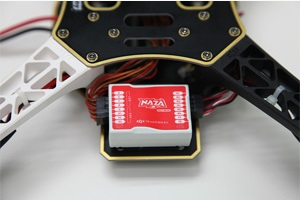
\includegraphics[width = 0.6\textwidth]{Bilder/NAZA_M-lite}
      \par\end{centering}
      \caption[Flightcontroller DJI NAZA-M lite]{Flightcontroller DJI NAZA-M lite\cite{NAZA_M-lite}}
      \label{NAZA_M-lite}
    \end{figure}

    \subsubsection{WLAN}
    Das WLAN-Modul RN171, welches von Microchip verkauft wird, bietet die Schnittstelle zwischen Server und Hexacopter. Die Daten können entweder vom Server gesendet
    und vom PIC empfangen werden oder umgekehrt.
    Das WLAM-Modul wird mit einer UART-Schnittstelle betrieben. Für eine Kommunikation sind also nur 2 Leitungen notwendig.
    Es bietet die Möglichkeit über eine Anwendung wie TeraTerm oder HTerm eingestellt zu werden, zusätzlich wird aber auch ein Webinterface angeboten, dieses muss jedoch zuvor
    aktiviert werden.

    \begin{figure}[tbh]
      \begin{centering}
        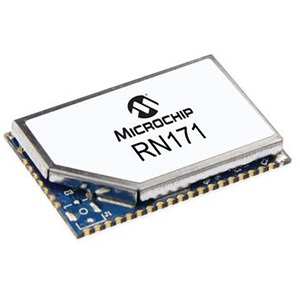
\includegraphics[width = 0.5\textwidth]{Bilder/RN171}
      \par\end{centering}
      \caption[WLAN-Modul RN171]{WLAN-Modul RN171\cite{RN171}}
      \label{RN171}
    \end{figure}

    Die Datenübertragung gestaltet sich dabei für den Nutzer sehr unproblematisch. Einerseits sind konfigurierbare Pins vorhanden um die Verbindung zu steuern und zu überwachen,
    andererseits braucht man sich nicht mehr um das Verpacken der Datenpakete kümmern.

%%%%%%%%%%%%%%%%%%%%%%%%%%%%%%%%%%%%%%%%%%%%%%%%%%%%%%%%%%%%%%%%%%%%%%%%%%%%%%%
\section{Blockschaltbild}
Die einzelnen Komponenten werden über den Mikrocontroller vereint. Sämtliche Berechnungen und Auswertung finden auf diesem statt und werden über diesen ausgegeben \bzw
weitergeleitet. Der Flightcontroller NAZA-M lite wird an die A, E, R und T Pins angeschlossen.
\begin{figure}[H]
  \begin{centering}
    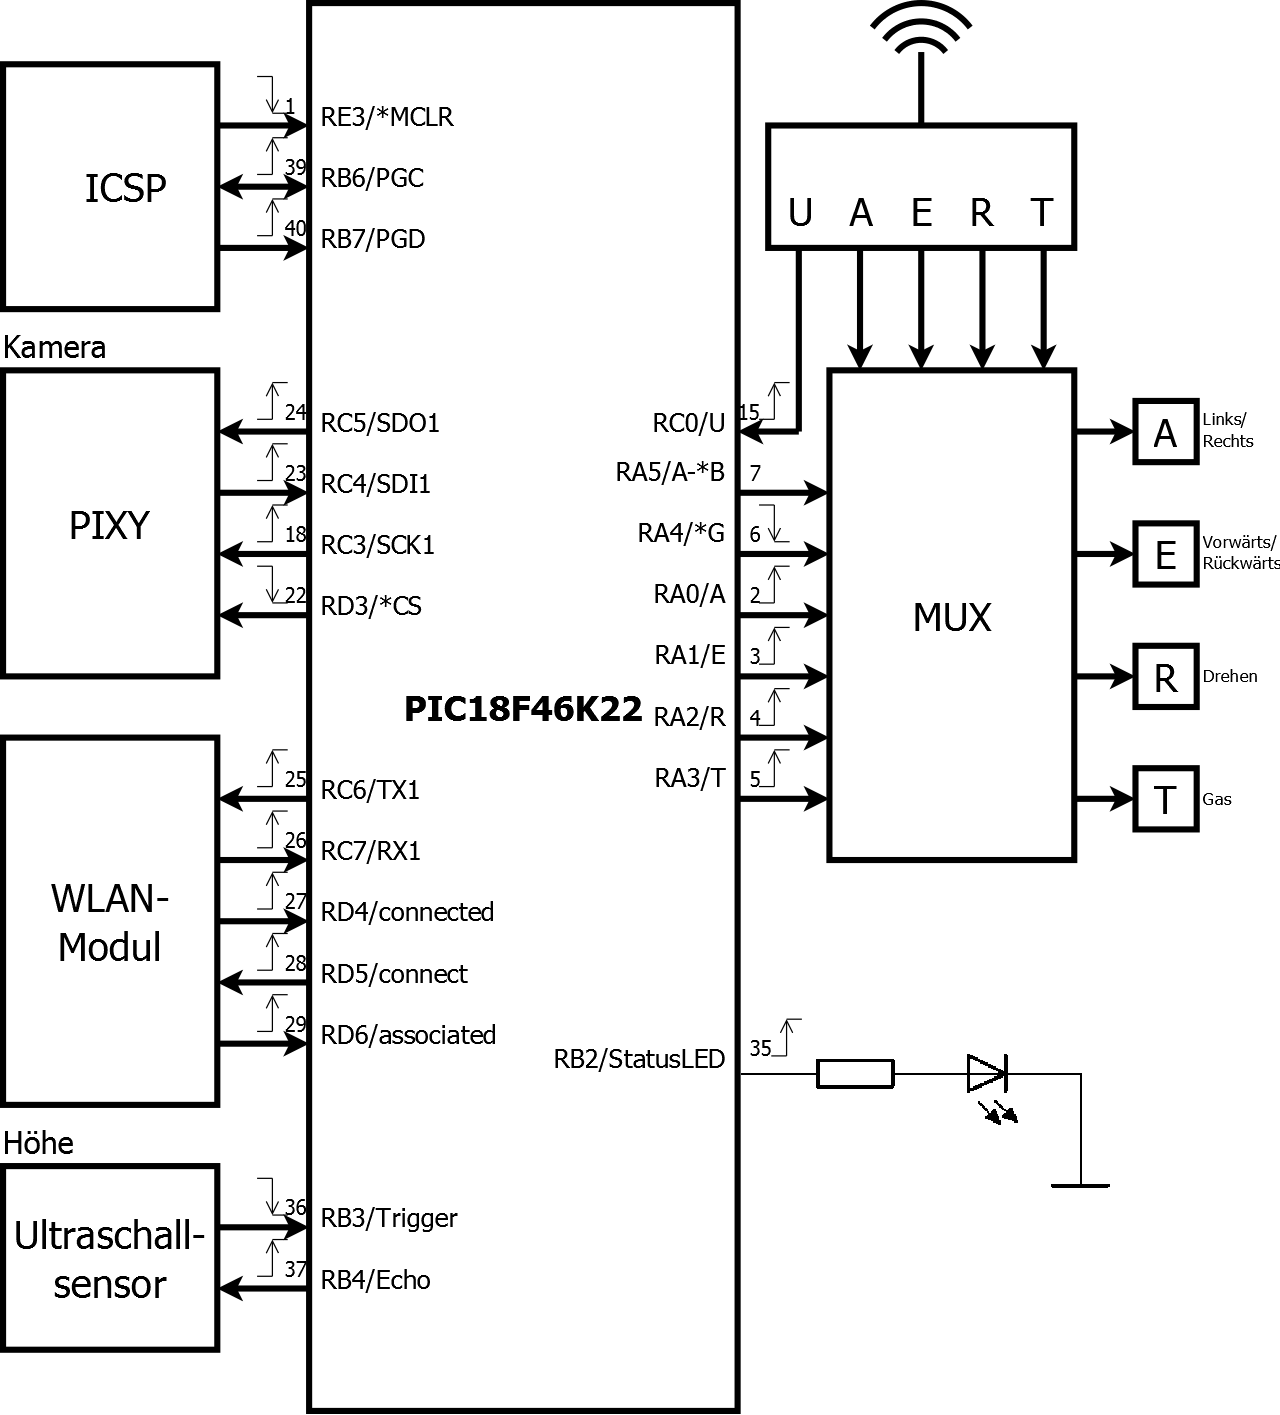
\includegraphics[width = 1\textwidth]{Bilder/Blockschaltbild}
  \par\end{centering}
  \caption{Blockschaltbild der Hauptplatine}
  \label{Blockschaltbild}
\end{figure}

  \subsection{Hauptplatine}
  Die Hauptplatine dient als zentrales Kommunikationselement. Auf ihr befindet sich der PIC welcher für sämtliche Berechnungen und Auswertungen zuständig ist.
  Um ein ausreichendes Maß an Kommunikationsfähigkeit zu ermöglichen, befinden sich auf ihr folgende Anschlüsse:
  \begin{itemize}
    \item $+\SI{5}{\volt}$ Spannungsversorgung
    \item Eingänge des Fernsteuerungsempfängers (5 Pins)
    \item Ausgänge zum Flightcontroller (4 Pins)
    \item Anschluss für den Ultraschallsensor
    \item Anschluss für die PIXY CMUcam5
    \item Anschluss für das WLAN-Modul
  \end{itemize}

    \subsubsection{Technische Planung}
    Das Hauptkriterium für die Hauptplatine war es alle notwendigen Komponenten für einen autonomen Flug zu enthalten. Wichtig waren hier vor allem die Kamera,
    der Ultraschallsensor sowie die Möglichkeit auf einen manuellen Flug zu wechseln.

    \subsubsection{Umsetzung}
    Für die Umsetzung wurden die einzelnen Komponenten entsprechend ihrer Funktion im Schalplan verbunden und aus diesem ein Platinen-Layout erstellt.
    Das Platinen-Layout wurde schließlich mit einem Fräsplotter auf das Rohmaterial übertragen.

    \begin{figure}[tbh]
      \begin{centering}
        \subfigure[Oberseite]{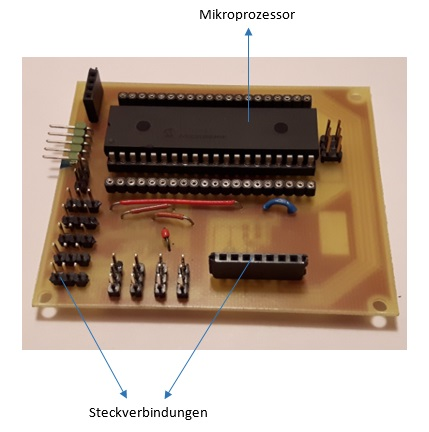
\includegraphics[width = 0.49\textwidth]{Bilder/HP_top}}
        \subfigure[Unterseite]{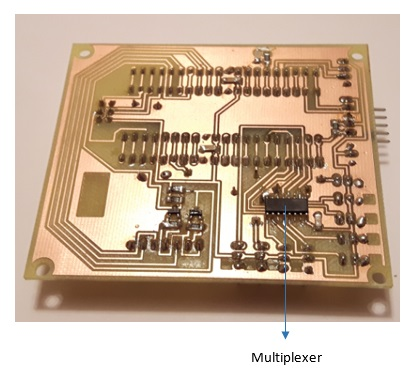
\includegraphics[width = 0.49\textwidth]{Bilder/HP_bot}}
      \par\end{centering}
      \caption{Die bestückte Hauptplatine}
      \label{Hauptplatine}
    \end{figure}

    \subsubsection{Herausforderungen und Lösungen}
    Eine Herausforderung stellte die geringe Deckkraft des schwarzen Toners beim ätzen der Platine dar. Durch zu wenig Toner auf der Belichtungsvorlage sind
    angeätzte Masseflächen entstanden. Um dennoch eine ordentliche Platine zu haben wurde diese schließlich gefräst. Dies hat auch viel Arbeit beim Bohren der
    Löcher erspart.

  \subsection{WLAN-Modul}
  Das WLAN-Modul dient als Schnittstelle zwischen Hauptplatine und Server. Auf dieser Platine befinden sich das WLAN-Modul RN171 sowie ein Spannungsregler und Level-Shifter
  um eine Kompatibilität mit den anderen Komponenten zu gewährleisten.

    \subsubsection{Technische Planung}
    In der Planung war die Versorgungsspannung des WLAN-Modul das Hauptaugenmerk. Für den Betrieb sind $\SI{3.3}{\volt}$ notwendig, die Versorgungsspannungstoleranz
    des WLAN-Moduls ist nicht groß genug, um dieses mit $\SI{5}{\volt}$ versorgen zu können.
    Aufgrund der fehlenden Toleranz müssen alle Leitungen die zur Kommunikation dienen entweder auf $\SI{5}{\volt}$ angehoben oder auf $\SI{3.3}{\volt}$ abgesenkt werden,
    andernfalls kann es zu Datenverlust oder sogar einer Beschädigung eines Moduls kommen.

    \subsubsection{Umsetzung}
    Auch für diese Platine wurde ein Schaltplan und Layout erstellt. Anschließend wurde das Layout wieder mit einem Fräsplotter auf das Rohmaterial übertragen.

    \begin{figure}[tbh]
      \begin{centering}
        \subfigure[Oberseite]{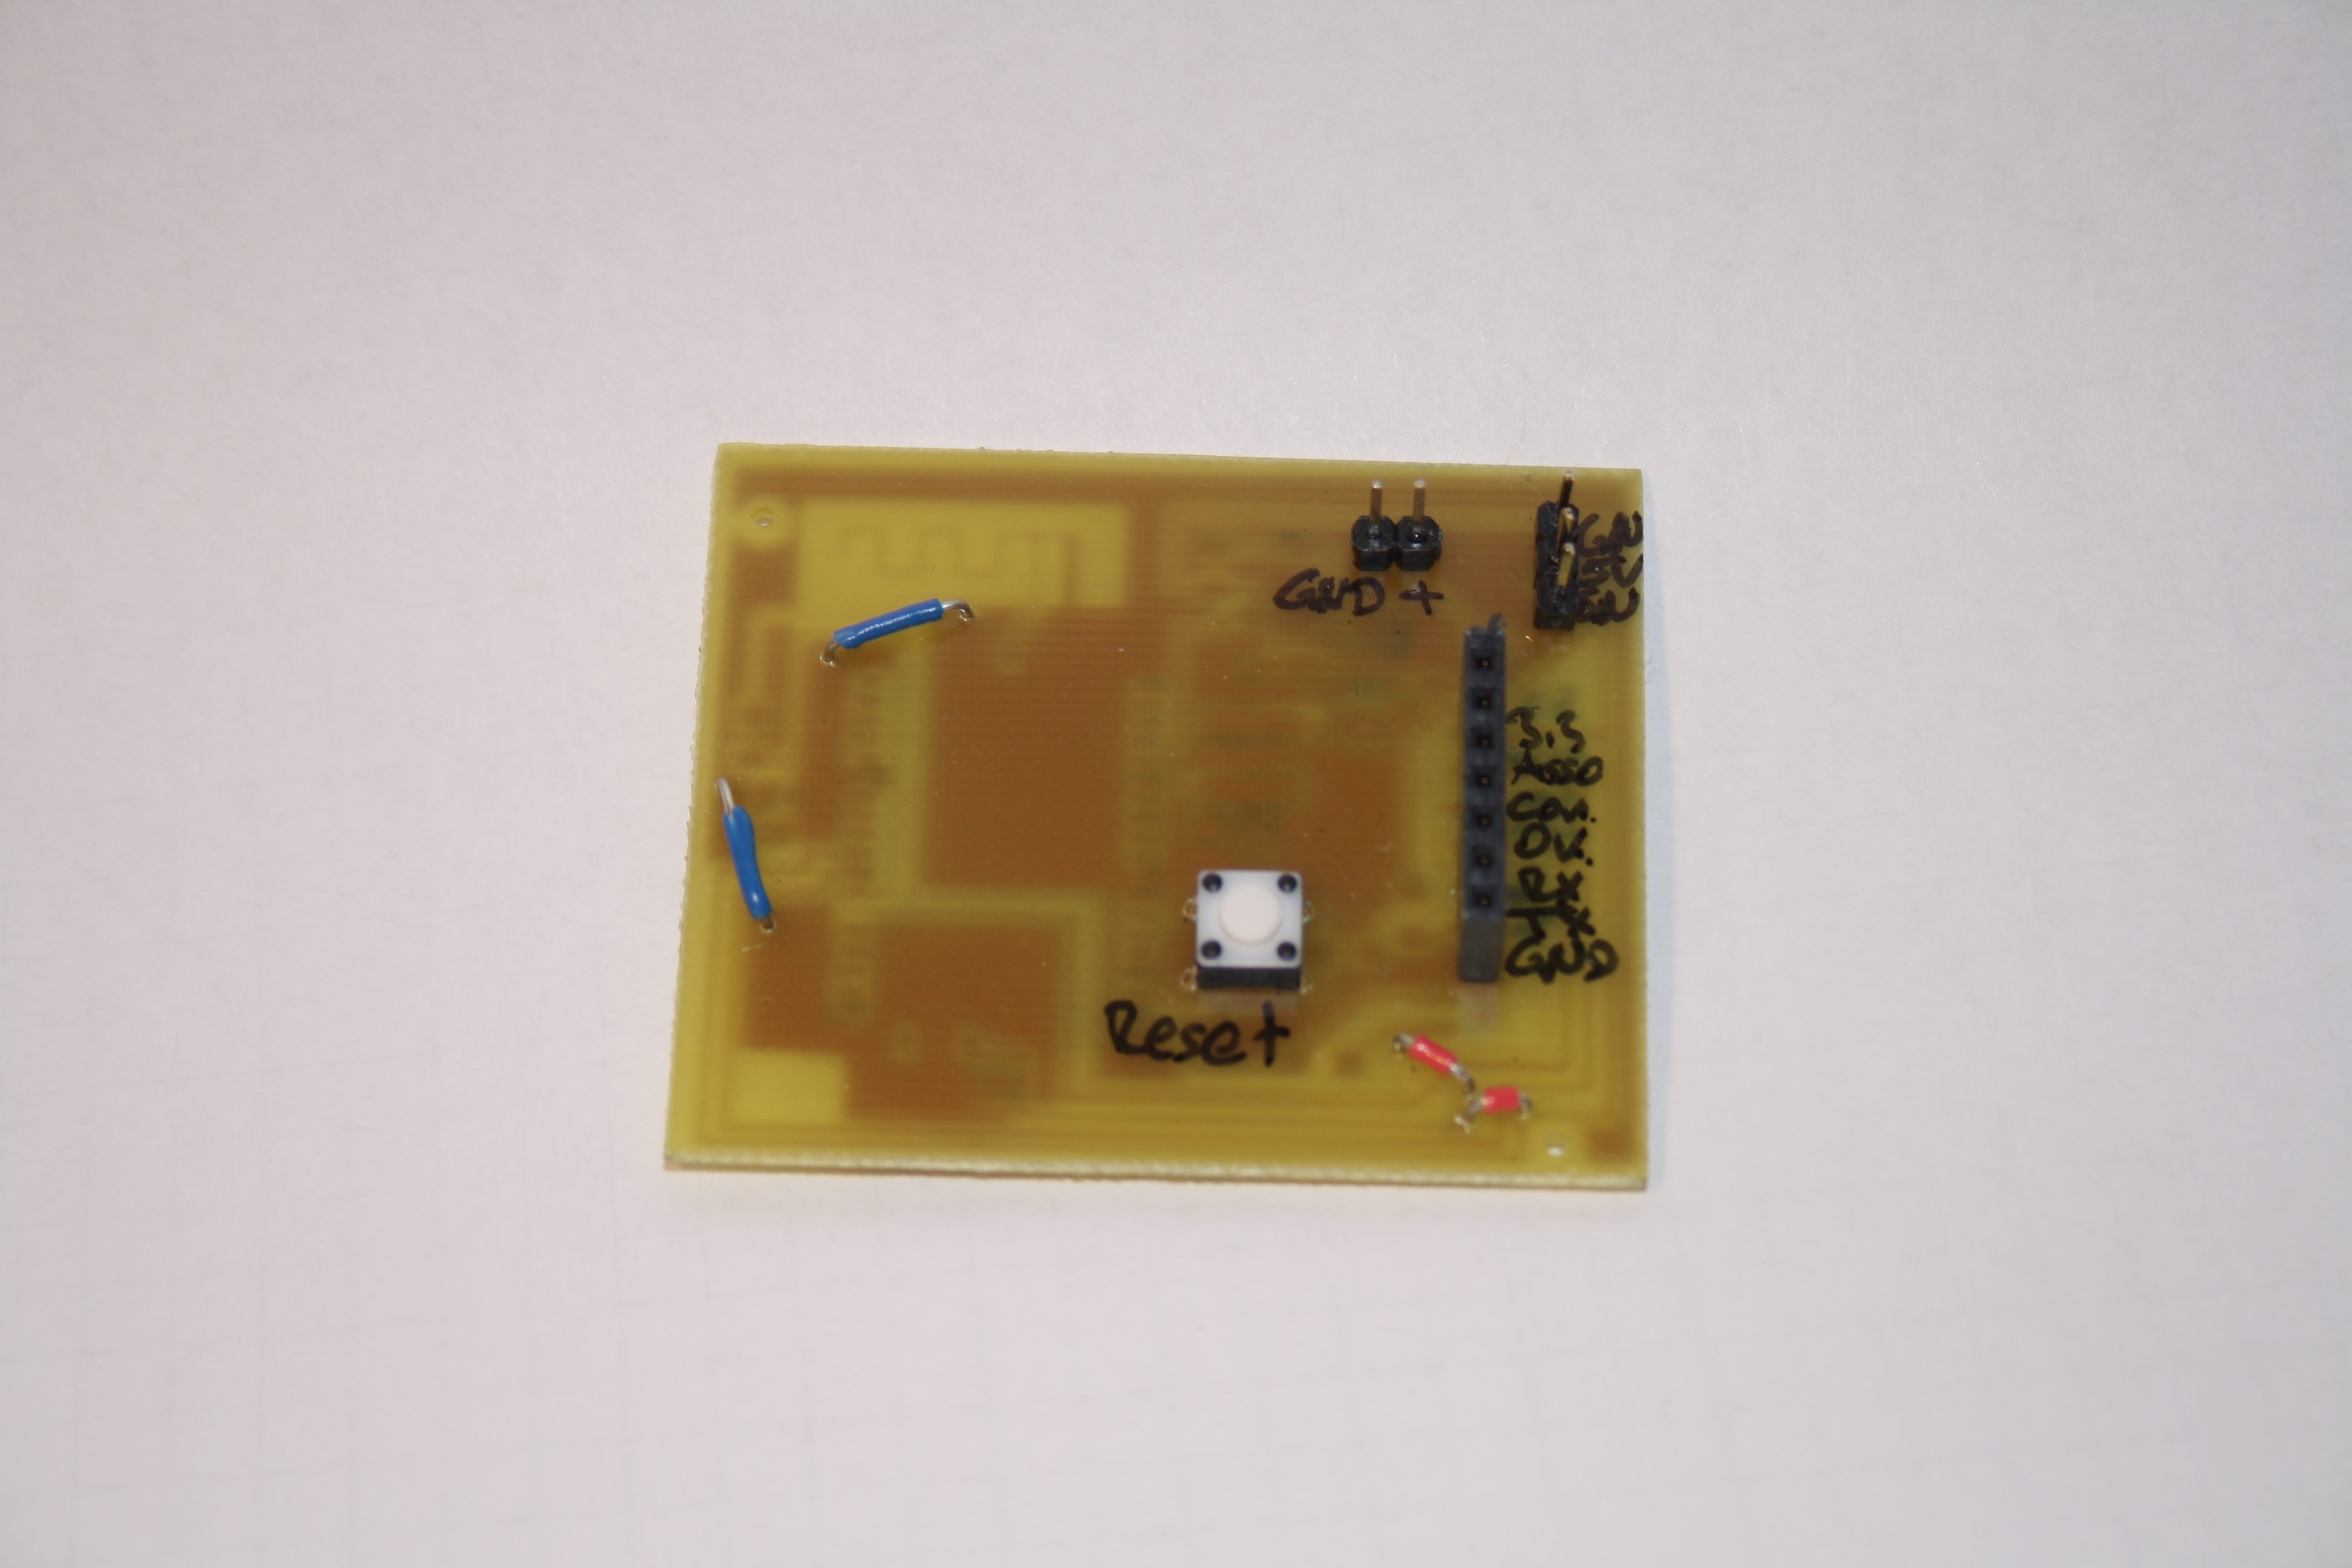
\includegraphics[width = 0.49\textwidth]{Bilder/WLAN_top}}
        \subfigure[Unterseite]{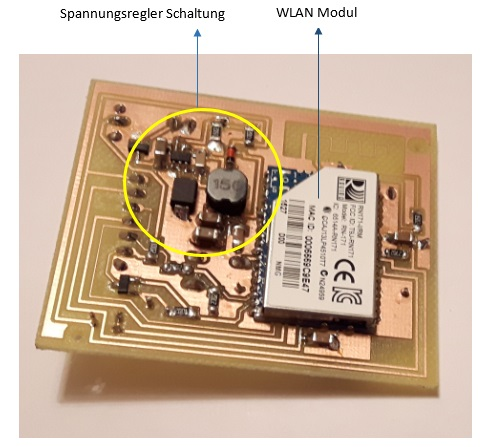
\includegraphics[width = 0.49\textwidth]{Bilder/WLAN_bot}}
      \par\end{centering}
      \caption{Die bestückte WLAN-Platine}
      \label{WLAN-Platine}
    \end{figure}

    %\begin{figure}
    %  \centering
    %  \begin{subfigure}[h]{0.49\textwidth}
    %    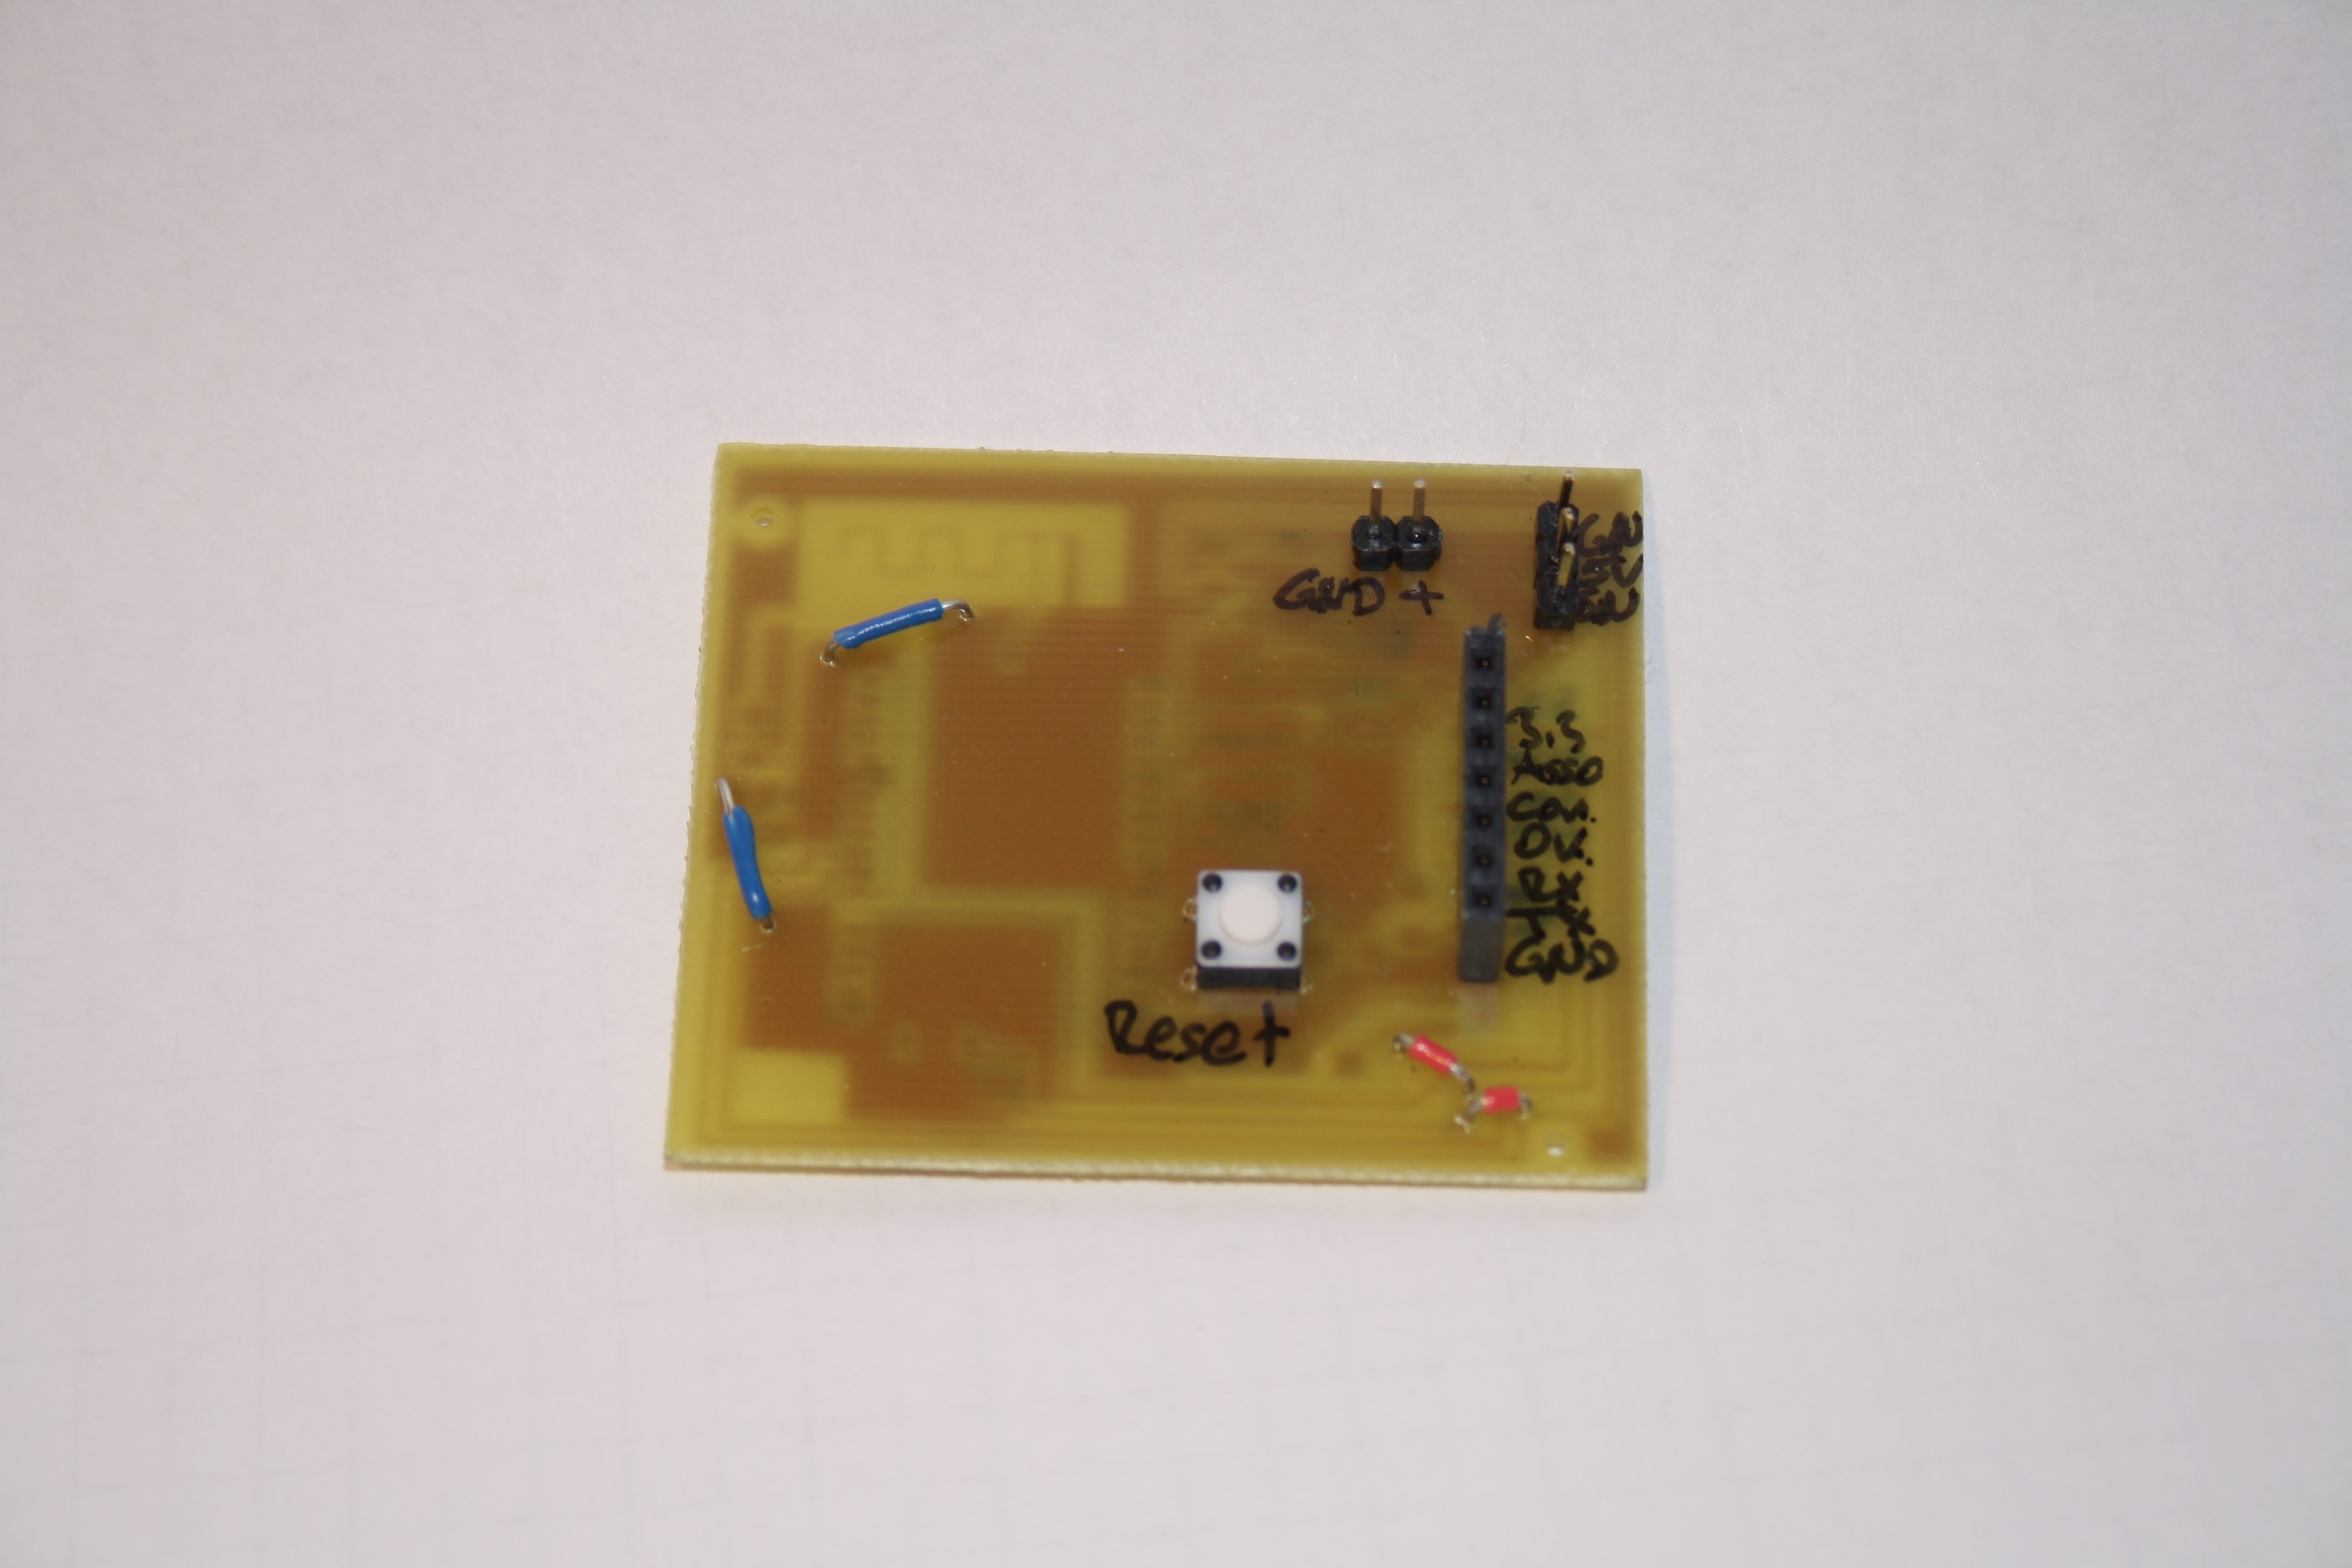
\includegraphics[width = \textwidth]{Bilder/WLAN_top}
    %    \caption{Oberseite}
    %  \end{subfigure}
    %  \begin{subfigure}[h]{0.49\textwidth}
    %    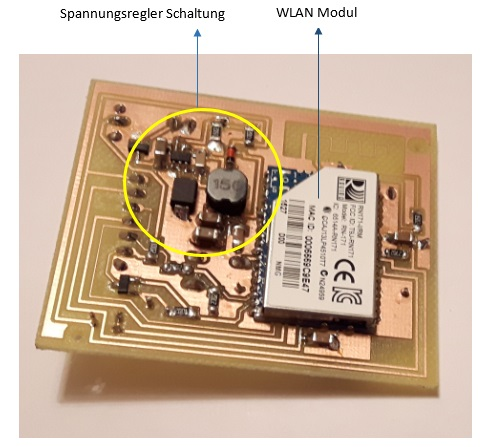
\includegraphics[width = \textwidth]{Bilder/WLAN_bot}
    %    \caption{Unterseite}
    %  \end{subfigure}
    %  \caption{Die bestückte WLAN-Platine}
    %  \label{WLAN-Platine}
    %\end{figure}

    \subsubsection{Herausforderungen und Lösungen}
    Um eine funktionierende Kommunikation sicher stellen zu können, wurden mehrere Level-Shifter in Richtung des Mikroprozessors sowie Spannungsteiler in Richtung des WLAN-Moduls
    integriert. Diese Maßnahmen sorgen dafür, dass weder das WLAN-Modul beschädigt wird, noch Daten verloren gehen.
    Bei der Platinen-Fertigung wurde aufgrund der schlechten Deckkraft abermals auf den Fräsplotter zurückgegriffen.


% !TEX root = diplomarbeit.tex
\chapter{Sensoren}
\renewcommand{\kapitelautor}{Autor: Lucas Ullrich}

%%%%%%%%%%%%%%%%%%%%%%%%%%%%%%%%%%%%%%%%%%%%%%%%%%%%%%%%%%%%%%%%%%%%%%%%%%%%%%%
\section{PIXY CMUcam5}
Bei der PIXY CMUcam5 handelt es sich um ein Open Source Kameramodul, welches über eine Objekterkennung verfügt.
Mit diesem ist es möglich sogenannte Colorcodes oder einfache Objekte zu erkennen.

\begin{figure}[H]
  \begin{centering}
    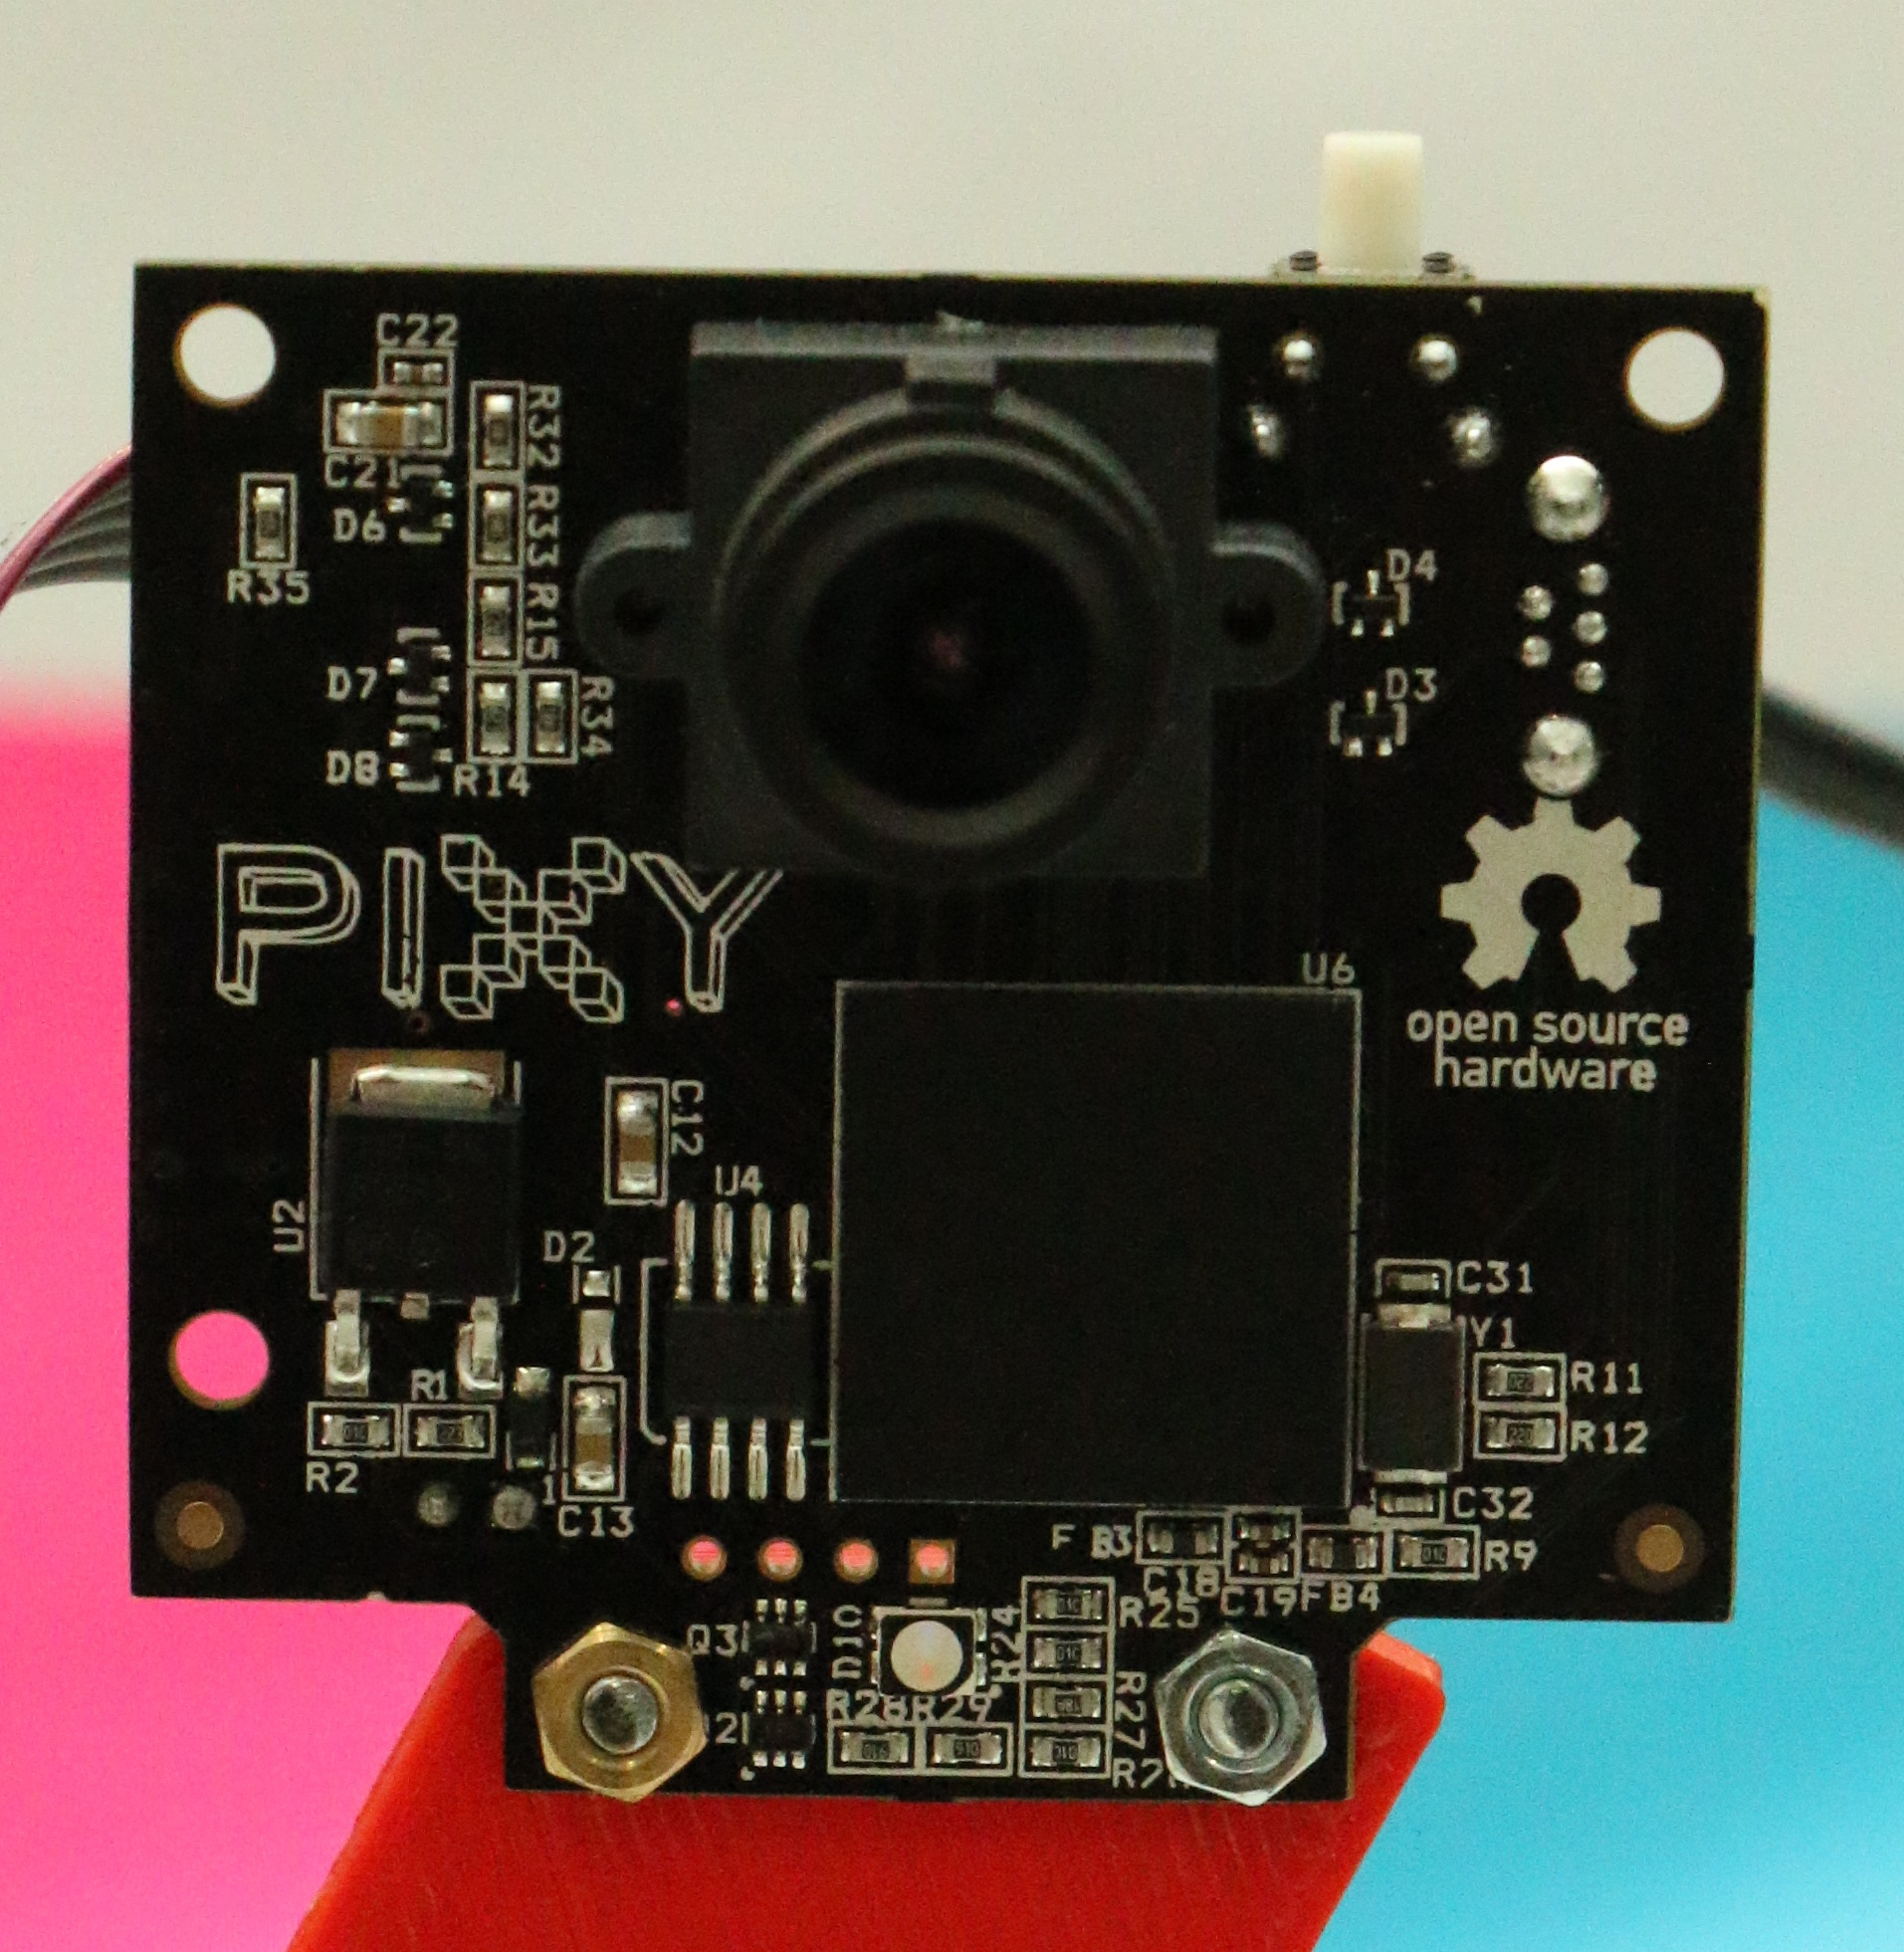
\includegraphics[width = 0.4\textwidth]{Bilder/Pixy_CMUcam5}
  \par\end{centering}
  \caption{PIXY CMUcam5}
  \label{PIXY}
\end{figure}

\begin{figure}[H]
  \begin{centering}
    \subfigure[Colorcode]{
\includegraphics[width = 0.4\textwidth]{Bilder/Colorcode}}
    \subfigure[Objekt]{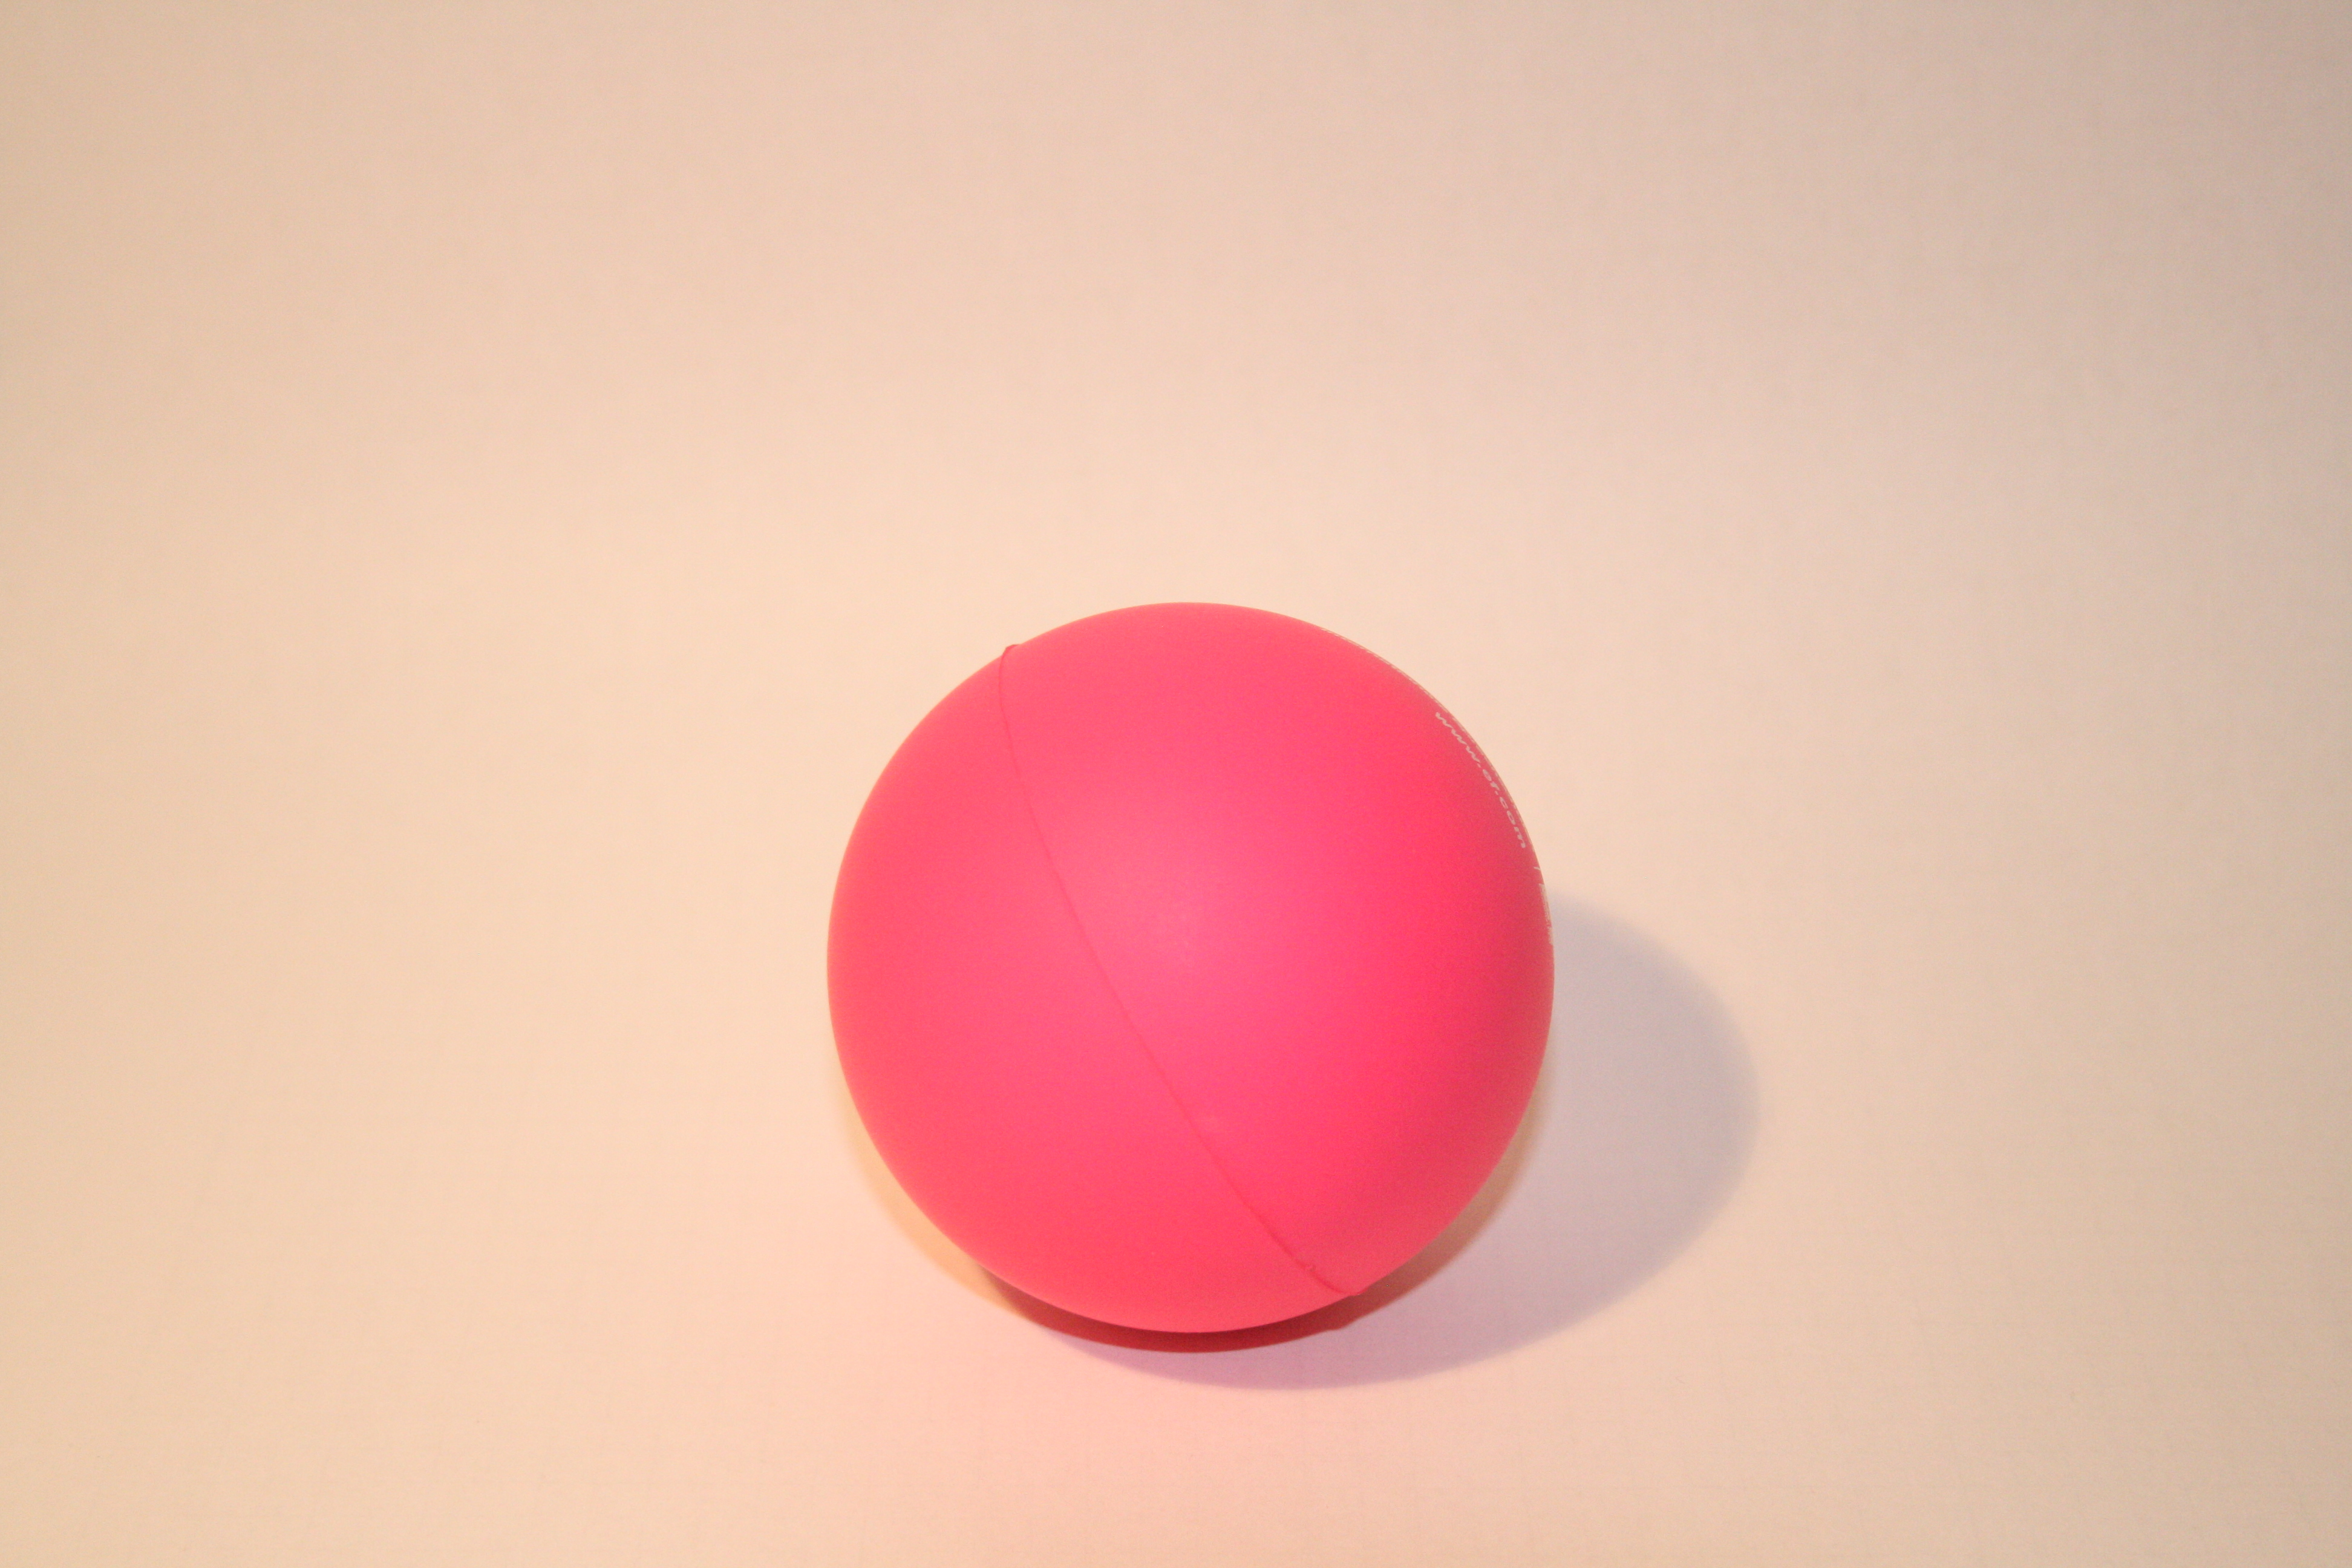
\includegraphics[width = 0.4\textwidth]{Bilder/Objekt}}
  \par\end{centering}
  \caption{Erkennbare Objekttypen}
  \label{PIXY_Objekte}
\end{figure}

\needspace{2cm}

  \subsection{Umsetzung}
  Durch die PIXY CMUcam5 lässt sich eine relative Positionsmessung vergleichsweise einfach verwirklichen.
  Werden ein oder mehrere Objekte erkannt wird eine bestimmte Nummer (abhängig von der Farbe) sowie die Position am Bild und die Objektgröße übermittelt.
  Die Kamera arbeitet dabei mit einer Bildwiederholrate von 50 Hz, es ist also alle 20 ms eine Auswertung möglich.

  Die Kamera wird auf dem Hexacopter befestigt, mehrere Farbcodes kennzeichnen den Weg zu einem Tisch.
  Um an dieser Stelle eine Navigation zu erreichen wird der Hexacopter so gesteuert, dass er, abhängig von der Route,
  immer einen bestimmten Farbcode betrachtet, ist er über diesem sucht er den nächsten.

    \subsubsection{SPI Schnittstelle}
    Als Schnittstelle für die Kommunikation mit der Kamera wird eine SPI-Schnittstelle verwendet.
    Die Kamera selbst unterstützt unter anderem die seriellen Schnittstellen UART, I2C und SPI.
    Außerdem werden noch ein analoger und digitaler Output unterstütz, diese sind jedoch vergleichsweise beschränkt,
    da keine näheren Informationen zu dem Objekt übermittelt werden können sondern nur die Position \bzw ob überhaupt ein Objekt erkannt wurde.

    Die SPI-Schnittstelle ist bei der Kamera besonders ausfallsicher. Hier wird ein Synchronisationsbyte gefordert, wird dieses nicht erkannt,
    \zB aufgrund eines Fehlers in der Datenübertragung, schickt die Kamera keine Daten.

    \subsubsection*{Überprüfen der SPI-Schnittstelle}
    Um zu überprüfen ob die SPI-Schnittstelle auch korrekt arbeitet, wird bei der ersten Inbetriebnahme der Output überprüft.
    Hierzu wird der Zustand der 3 Leitungen mit einem Oszilloskop betrachtet.
    \begin{itemize}
      \item \textcolor{blue}{Taktleitung}
      \item \textcolor{red}{Dateneingang (PIC)}
      \item \textcolor{green}{Datenausgang (PIC)}
    \end{itemize}

    \begin{figure}[tbh]
      \begin{centering}
        \subfigure[Großer Zeitbereich]{\includegraphics[width = 0.49\textwidth]{Bilder/SPI_gross}}
        \subfigure[Kleiner Zeitbereich]{\includegraphics[width = 0.49\textwidth]{Bilder/SPI_klein}}
      \par\end{centering}
      \caption{Ausgang der SPI Schnittstelle}
      \label{SPI-Ausgang}
    \end{figure}

    Der Wert mit dem diese Überprüfung durchgeführt wird, sollte möglichst variabel sein, hier wird 0xAA (1010 1010) verwendet.
    Wird dieser Wert nicht variabel angenommen, kann es dazu kommen, dass fälschlicher Weise angenommen wird, dass die Übertragung korrekt ist. Dies kann durch externe Faktoren wie
    Pull-Up-Widerstände oder Default-Status einer Leitung geschehen, in beiden Fällen würde je nach Schnittstelle "1" oder "0" übertragen werden, dies wäre falsch.

    Der Dateneingang des PIC, respektive der Ausgang der Kamera, zeigt eine deutliche Störung durch die Taktleitung an.

    \subsubsection{Erkennen und Auswerten eines Bildes}
    Die Kamera schickt der Reihe nach die einzelnen Daten eines Objekts. Darunter ist auch ein Startwort welches ein neues Bild markiert.
    Mit den diversen Informationen zum Objekt ergeben sich folgende Daten:
    \begin{itemize}
      \item Neues Bild 0xAA55
      \item Objekt 0xAA55 oder Farbcode 0xAA56
      \item Checksum
      \item Objektnummer
      \item X-Position
      \item Y-Position
      \item Breite
      \item Höhe
      \item Drehwinkel, nur bei Farbcodes
    \end{itemize}
    Dabei ist die Objektnummer von den im Objekt oder Farbcode vorkommenden Farben abhängig, zusätzlich ist zu beachten, dass sie oktal dargestellt wird.
    Ein übermittelter Wert von dezimal 10, also oktal 12, bedeutet, dass die Farben 1 und 2 erkannt wurden.

    Will man nun ein neues Bild finden, muss man so lange nach 0xAA55 suchen bis man diese Daten gesendet bekommt.
    Anschließend gilt es noch festzustellen ob man einen Farbcode oder ein Objekt betrachtet,
    es muss also direkt darauf 0xAA56 oder nochmals 0xAA55 erkannt werden. Ist dies nicht der Fall, wurde kein neues Bild erkannt und man betrachtet ein normales Objekt.

    Betrachtet man nun die bis zum Erkennen eines neuen Bildes gesendeten Daten als gegenstandslos, ergibt sich eine vergleichsweise einfache Schleife um ein Bild zu erkennen.

    \lstset{language = c}
    \begin{lstlisting}
while(frame == 0) {
  w = ExchangeSpiWord(PIXY_SYNC, DUMMY);
  if(lw == PIXY_FRAME_OBJ && w == PIXY_FRAME_OBJ) {
    frame = 1;
    obj_type = 0;
    a_color[c_obj].type = PIXY_FRAME_OBJ;
  } else if(lw == PIXY_FRAME_OBJ && w == PIXY_COLORCODE) {
    frame = 1;
    obj_type = 1;
    a_color[c_obj].type = PIXY_COLORCODE;
  } else if(w == 0 && lw == 0){
    frame = 0;
  }
  lw = w;
  c++;
  if(c > 254) {
    return 0;	//****Error, end of function
  }
}
    \end{lstlisting}
    Um nicht ewig in dieser Schleife fest zu hängen, wenn kein Bild erkannt wird und einen Fehler auslösen zu können wird die gesamte Funktion der Bildauswertung
    nach 255 Versuchen verlassen.

    Die weiteren Werte eines Objekts werden der Reihe nach in einer \gls{Struktur} abgespeichert, hier ist nichts Besonderes mehr zu beachten.

  \subsection{Herausforderungen und Lösungen}
  Insbesondere das Beispielprogramm\cite{PIXY_Porting_Examplecode} für eine Bildauswertung stellte einige Herausforderungen dar. Hier sind unterschiedliche Codeschnippsel in einem
  großen Beispiel zusammengefasst. Die große Ähnlichkeit verschiedener Funktionen erschweren die Lesbarkeit des Codes erheblich. So steht eine Funktion für die Erkennung eines
  neuen Bildes, diese zählt aber nur Bilder pro Sekunde, eine andere ist dann für die gesamte Auswertung und sucht dafür erneut nach einem Bild.

  Diese Zusammenhänge konnten durch einige Überlegungen erkannt werden und darauffolgend die eigene Firmware geschrieben werden.

  Ein weiteres Problem stellt die Empfindlichkeit der Kamera bei wechselnden Lichtverhältnissen dar. Da diese über die Farbsignatur eines Objektes arbeitet, werden bereits
  sehr kleine Differenzen unterschieden um verschiedene Objekte erkennen zu können \bzw keine Störungen durch den Hintergrund zu erhalten. Dies wird jedoch ebenso in der
  anderen Richtung zu einem Problem. Wechselt das Licht ein wenig kann ein Farbcode oft nicht mehr zuverlässig erkannt werden und die Kamera muss über einen Computer nachkalibriert
  werden. Eine mögliche Lösung ist das konstante Beleuchten der Farbcodes mit einer sehr bestimmten Leuchtstärke, hier kann es leicht zu Überbelichtungen kommen, sowohl bei
  dunklen Verhältnissen, als auch die Umrüstung auf einen \gls{Infrarot}-Kit. Bei einem Infrarot-Kit fällt jedoch die Individualität jedes einzelnen Markers weg.

%%%%%%%%%%%%%%%%%%%%%%%%%%%%%%%%%%%%%%%%%%%%%%%%%%%%%%%%%%%%%%%%%%%%%%%%%%%%%%%
\section{Ultraschallsensor HC-SR04}
Der Ultraschallsensor HC-SR04 ist ein für Arduino entwickeltes Modul um Abstände zu messen. Die Messung geschieht durch das Aussenden von Ultraschallimpulsen,
die Messgröße wird dabei als laufzeitabhängiger Impuls retourniert.

\begin{figure}[tbh]
  \begin{centering}
    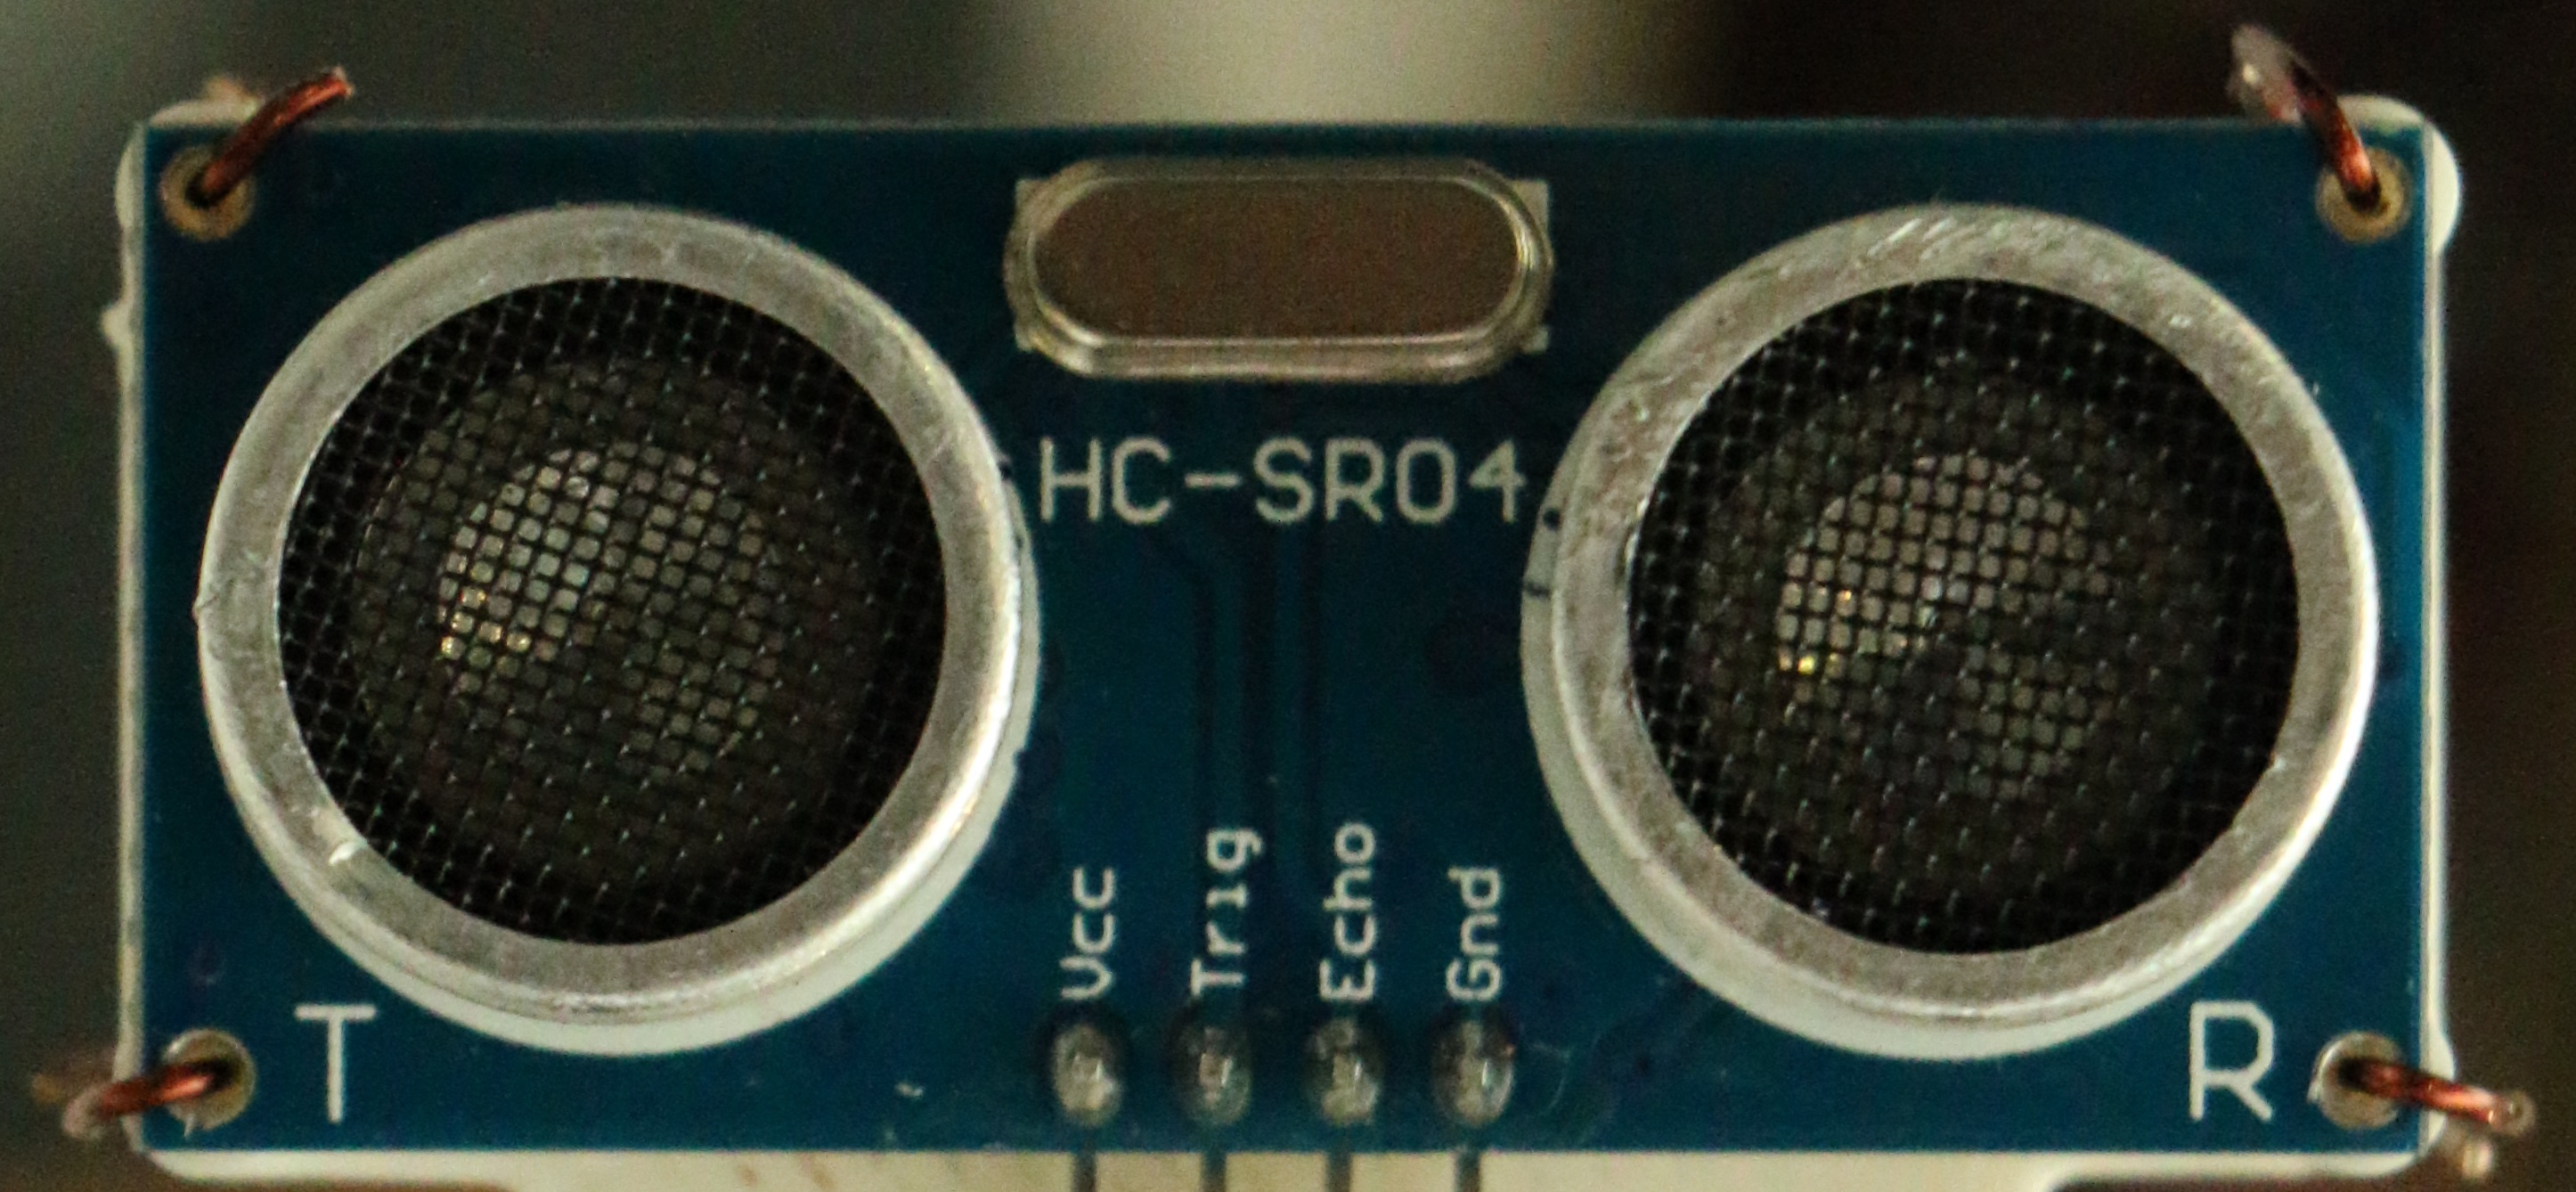
\includegraphics[width = 0.5\textwidth]{Bilder/Ultraschallsensor}
  \par\end{centering}
  \caption{Ultraschallsensor HC-SR04}
  \label{Ultraschallsensor}
\end{figure}

  \subsection{Technische Planung}
  Für die Steuerung des Hexacopter ist es notwendig die aktuelle Flughöhe zu wissen.
  Es ist mit einer bekannten Objektgröße und den von der Kamera vorliegenden Daten zwar möglich die aktuelle Flughöhe rechnerisch zu bestimmen,
  jedoch gestaltet sich dies sehr rechenaufwändig \bzw ungenau. Um die Höhe möglichst einfach messen zu können bietet sich daher eine vergleichsweise langsame Messung,
  wie jene mit einem Ultraschallsignal an.
  Bei einer Schallgeschwindigkeit von $\SI{343}{\meter\per\second}$ entstehen bei einer zu messenden Distanz von $\SI{2}{\meter}$,
  Laufzeiten des Ultraschallsignals von \ca $\SI{12}{\milli\second}$ (Distanz mal 2 da das Signal wieder zurückkehren muss).

  \subsection{Umsetzung}
  Abhängig von der mit dem Mikroprozessor ermittelten Laufzeit $time\_height$ lässt sich jederzeit die aktuelle Flughöhe bestimmen.
  \[
  s(time\_height) = \frac{v \cdot t}{2} = \frac{\SI{343}{\meter\per\second} \cdot time\_height}{2}
  \]
  Die Höhe wird dabei in der main-Routine durch den Aufruf folgender Funktionen regelmäßig bestimmt:
  \lstset{language = c}
  \begin{lstlisting}
void StartHeightMeasure(void) {
  TMR5L = 0;
  TMR5H = 0;
  Trigger = 0;
}

void ReadHeight(void) {
  while(TMR5GIF == 0);
  TMR5GIF = 0;
  time_height = 0;
  time_height = TMR5H;
  time_height <<= 8;
  time_height |= TMR5L;
  TMR5L = 0;
  TMR5H = 0;
  a_frame[0].height = time_height;
  a_frame_dif[0].dif_height = a_frame[1].height - a_frame[0].height;
  Trigger = 1;
}
  \end{lstlisting}

  In der ersten Funktion wird die Messung gestartet. Dazu wird ein Trigger-Signal an den Ultraschallsensor gesendet, dieser reagiert auf eine fallende Flanke.
  Zuvor wird darauf geachtet, dass die Register in denen die Zeit zurückgegeben wird auch wirklich leer (= 0) sind.
  In der zweiten Funktion folgt das Auslesen der vorhandenen Daten. Dazu werden die zwei 8-Bit Register in der 16-Bit Variable $time\_height$ abgespeichert.
  Zusätzlich wird die gemessene Höhe für die Auswertung in der $a\_frame[0].height$ Variable abgespeichert und die Differenz zur vorhergehenden Messung ermittelt.

  Auf eine Berechnung der genauen Höhe in m wird zu Gunsten der Verarbeitungszeit verzichtet, auf die spätere Auswertung der Flugdaten hat dies keinen Einfluss.

  \subsection{Herausforderungen und Lösungen}
  Bei der Verwendung des Ultraschallsensors traten einige Herausforderungen auf. So war bei einem der Testflüge ersichtlich, dass Throttle von der Firmware auf der Hardware nicht mehr
  zurück genommen wird, in der Simulation hingegen schon. Der erste Verdacht fiel auf eine verfälschte Messung im Betrieb, deshalb wurde in das Programm ein Teil implementiert, der
  es ermöglicht die gemessenen Werte über WLAN auf einen Computer zu übertragen.
  \lstset{language = c}
  \begin{lstlisting}
#ifdef DEBUG
void SendDebugInfo(unsigned int debug_info) {
    for(unsigned char debug_info_counter = 0;
      debug_info_counter < 5; debug_info_counter++) {
        send_info[debug_info_counter] = debug_info % 10;
        debug_info = ( debug_info - send_info[debug_info_counter]) / 10;
    }
    for(signed char debug_send_counter = 4;
      debug_send_counter >= 0; debug_send_counter--) {
        unsigned char send = send_info[debug_send_counter];
        UartSendAscii(send);
    }
    UartSend(';');
}
#endif
  \end{lstlisting}

  Um dieses nach der Verwendung wieder einfach aus dem Code entfernen zu können wurde das Übermitteln dieser Information an die Definition der $DEBUG$-Variable geknüpft.

  In der Übertragung war es wichtig auf die Auswertung des Computers zu achten, desshalb mussten ASCII-Zeichen übertragen werden.

  Die erste Messung bestätigte die Erwartungen:
  \begin{figure}[H]
    \begin{centering}
      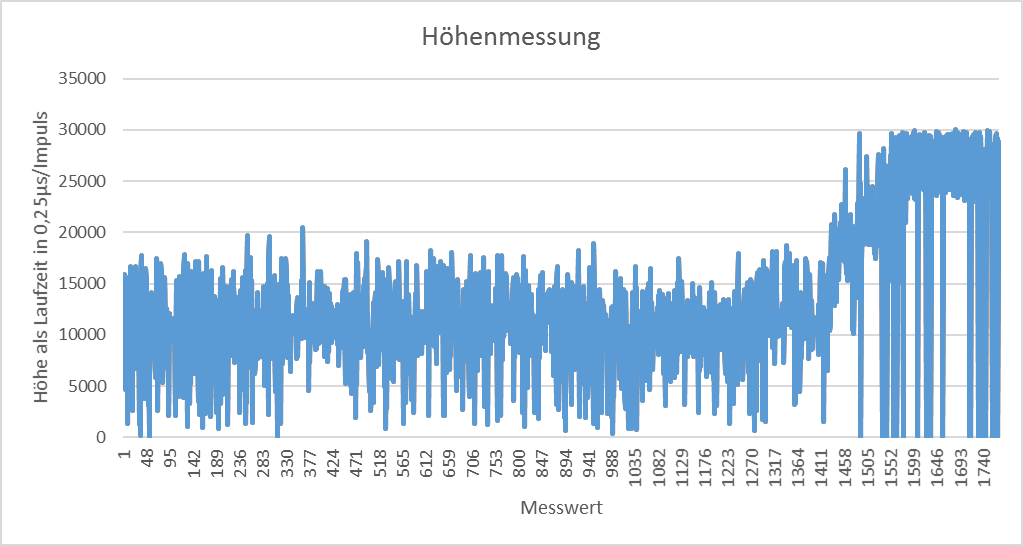
\includegraphics[width = 0.8\textwidth]{Bilder/Hoehenmessung}
    \par\end{centering}
    \caption{Höhenmessung während einem Flugvorgang}
    \label{Hoehenmessung}
  \end{figure}
  Die Messung wurde während einem manuellen Flug gestartet, die Gasstellung war auf mehr als Schwebeflug, und wurde mit einer Landung beendet. Der Hexacopter wurde dabei ständig
  auf der selben Höhe gehalten, die Messwerte änderten sich dennoch und zeigten eine Änderung der Flughöhe an.

  Als Grund wurden erst Störungen des Ultraschallsensors durch Geräusche des Hexacopters vermutet, dies konnte jedoch nicht bestätigt werden, hingegen dessen führten Vibrationen
  zu den falschen Messwerten. Um die Vibrationen nahezu vollständig zu beseitigen wurde der Sensor gedämpft gelagert und ebenso das Kabel anders verlegt.
  \begin{figure}[H]
    \begin{centering}
      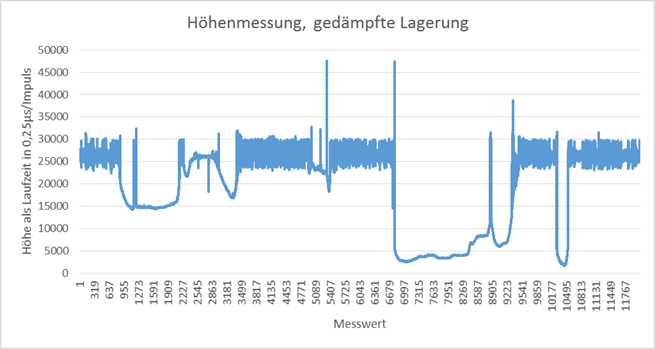
\includegraphics[width = 0.8\textwidth]{Bilder/Hoehenmessung_gedaempft}
    \par\end{centering}
    \caption{Gedämpfte Höhenmessung während einem Flugvorgang}
    \label{Hoehenmessung_gedaempft}
  \end{figure}
  Das Ergebnis zeigt, während einem Flug, deutlich stabilere Werte, eine Annäherung zum Boden wird ebenso sehr zuverlässig erkannt. Lediglich bei der Messung der Distanz in einer Flughöhe
  von \ca $\SI{1.3}{\meter}$ (Ausgangsposition für die Messungen) zeigen sich starke Schwankungen.

\chapter{Aktoren}
\renewcommand{\kapitelautor}{Autor: Christina Bornberg}

%%%%%%%%%%%%%%%%%%%%%%%%%%%%%%%%%%%%%%%%%%%%%%%%%%%%%%%%%%%%%%%%%%%%%%%%%%%%%%%
\section{Multicopter}
  Multicopter gehören zu der Luftfahrzeuggattung Hubschrauber. Sie starten senkrecht und können durch den Antrieb der Rotoren Neigung erzeugen. Durch diese Neigung kann der Hexacopter nach vorne, zurück, nach links und nach rechts fliegen. Durch die Rotoren, bei denen sich abwechselnd einer nach links und einer nach rechts dreht, kann sich der Hexacopter zusätzlich um seine Hochachse drehen.

  \subsection{Funktion}
  Ein Multicopter besteht im Normalfall aus folgenden Komponenten:
  Dem Empfängermodul, dem DJI NAZA-M Flightcontroller sowie der Multicopterhardware (Rotoren, Motoren, Gestell und Leistungselektronik). Der Empfänger des Multicopters kann von einem Sender Steuersignale empfangen und aufgrund der empfangenen Steuersignale Soll-Werte für die Motoren berechnen, um den Multicopter auf die entsprechende Höhe bzw. entsprechende Geschwindigkeit in x, y oder z Richtung zu bringen.

  % BILD Funktion Blockschaltbild (Dokument) %

  \subsection{Erweiterte Funktion}
  Im Rahmen dieser Diplomarbeit wurden die üblicherweise verwendeten Teile um vier weitere Komponenten erweitert, um einen automatischen Flug zu gewährleisten: Pixycam, Ultraschallsensor, WLAN Modul und ein Mikrocontroller. Pixycam und Ultraschallsensor sind dafür verantwortlich, die Daten für die Berechnung der augenblicklichen Position des zu bestimmen. Im Mikrocontroller läuft ein Algorithmus, der aus diesen empfangen Daten die Position überprüft. Wenn der Wert vom optimalen Bereich abweicht, werden die Steuersignale abgeändert. Durch das Wlan-Modul bekommt der Mikrocontroller die Information, durch wie viele Marker der Weg definiert ist und welcher Farbcode der letzte ist, auf dem die Landung erfolgt.

  % BILD %

  \subsection{Multicopter Arten}
  Es gibt verschiedene Arten von Multicoptern. 

  Je nachdem wie viele Rotoren in einer Ebene liegen, setzt sich der Name zusammen.
  Die bekannteste Art ist der Quadrocopter, welcher 4 Rotoren besitzt. Weiters gibt es Hexacopter mit 6 und Octocopter mit 8 Rotoren. \cite{GrundlagenMulticopter}

  Der Flightcontroller DJI Naza-M lite unterstützt verschiedene Konfigurationsarten von Quadrocoptern und Hexacoptern. Hierzu zählen + und x Konfiguration für den Quadrocopter. Beim Hexacopter gibt es die Varianten +, x, reverse Y und Y. Diese werden im nächsten Abschnitt genauer beschrieben. \cite{NAZA_Konfig}

  \subsection{Konfiguration}
  Grundsätzlich gibt es 2 Arten einen Multicopter zu Konfigurieren. \cite{GrundlagenMulticopter}
  Einerseits die +- beziehungsweise I-Konfiguration, andererseits die x- beziehungsweise H-Konfiguration. Weiters gibt es die weniger verbreitete Y-Konfiguration. Dabei geht es um die Ausrichtung und die damit verbundene Fluglage.

  Für diese Diplomarbeit wurde die + Konfiguration für Hexacopter gewählt.

  Wie auf folgender Grafik ersichtlich ist, gibt es nach links und nach rechts drehende Rotoren. Die rot gekennzeichneten Arme geben an, wo die Vorderseite des Multicopters ist. Bei der Y-Konfiguration sind die blau Makierten Propeller oben, die Roten unten.

  % BILD mit 4, 6, 8 in + bzw x %

  \subsection{Mögliche Anwendungsgebiete}
  Multicopter finden in vielen Bereichen Anwendung. \cite{copterAnwendung}
  \begin{itemize}
    \item Fotographie und Videos / Filmindustrie / Anfertigen von hoch aufgelösten Luftbildkarten
    \item Multicopter als Hobby / Kunstflug
    \item Lagerhallen und Logistik / Bestands- und Inventaraufnahmen im Straßenbau
    \item Forschung / Schwarmverhalten
    \item Multicopter als Lebensretter / Rettungseinsätze / Katastrophenschutz
    \item Unterstützung der Polizei / große Menschenmengen überwachen
    \item Unbemannter Aufklärer bei Spezialeinheiten
    \item Kontrolle, Inspektion und Dokumentation von Brücken, Gebäuden, Gräben
    \item Militärische Anwendung: Spionagedrohne zur Aufklärung, Kampfdrohne zur Zerstörung, Rettungungsdrohne für Hilfsaktionen
  \end{itemize}


\section{Rotoren}

  \subsection{Technische Planung}
  Autor: Lucas Ullrich\\
  Der Hexacopter selbst vefügt über 6 Rotoren. Diese werden für die unterschiedlichen Flugrichtungen von dem Flightcontroller angesteuert.
  Der Flightcontroller liest die Daten an den einzelnen Steuerpins als Servo-Impulse ein. Die Daten werden dabei in einer Periode von $\SI{20}{\milli\second}$ gesendet.
  Die Information selbst liegt in den ersten $\SI{2}{\milli\second}$. Für den Impuls beträgt die Mittelstellung $\SI{1.5}{\milli\second}$, das Minimum $\SI{1}{\milli\second}$
  und das Maximum $\SI{2}{\milli\second}$. Das Signal folgt somit den Konventionen eines Servo-Impulses.

  \textcolor{red}{OSZIBILD: min, max Impuls}


    \subsubsection{Steuerungsarten}
    AUtor: Christina Bornberg\\
    Der Flightcontroller DJI NAZA-M lite wird über die Befehle Aileron, Elevator, Rudder und Throttle gesteuert. Zusätzlich gibt es den 2/3-position mode channel, der für das Umschalten mehrerer Modei zuständig ist. Handelsübliche Fernbedienungen verfügen über die selben Steuerbefehle. \cite{GrundlagenMulticopter}

      \begin{itemize}
        \item \textbf{A: Aileron} auch Rollen (engl. roll) genannt, ist für die Bewegung nach Links und Rechts zuständig.
        Um diese auszuführen, werden bei der Beschleunigung nach links, die rechten Propeller stärker betrieben, umgekehrt drehen sich die auf der linken Seite befindlichen Propeller beim Flug nach rechts schneller. Durch die entstehende Neigung, fliegt der Hexacopter in die gewünschte Richtung.
        \item \textbf{E: Elevator} auch Nicken (engl. pitch) genannt, ist für die Vorwärts- und Rückwärtsbewegung zuständig.
        Beim nach vorne und nach hinten fliegen, werden ebenfalls die rotoren schneller betrieben, die auf der jeweils gegenüberliegenden Seite liegen.
        \item \textbf{R: Rudder} auch Gieren (engl. yaw) genannt, ist für die Rotation an der Hochachse zuständig.
        Um den Hexacopter um seine eigene Hochachse rotieren zu lassen, werden für eine Rotation nach rechts, die rechts-drehenden Rotoren schneller betrieben, bei der Rotation nach Links, die links-drehenden.
        \item \textbf{T: Throttle} reguliert die Höhe.
        Bei gleichmäßiger Ansteuerung der 6 Rotoren, kann man je nach Drehgeschwindigkeit die Höhe verändern. Der Hexacopter fliegt bei stärkerer Beschleunigung nach oben, ansonsten sinkt er. Dies wird auch als Uplift and Downfall bezeichnet.
        \item \textbf{U: 2/3-position switch channel} ist zum Umschalten von zwei oder drei Steuermodi zuständig. Im Fall unserer Diplomarbeit wird zwischen autonomem und manuellem Flug gewechselt. \cite{positionswitch}
      \end{itemize}

    % BILD Fernsteuerung%

  \subsection{Umsetzung}
  Um den Hexacopter steuern zu können müssen die einzelnen Impulse von dem Mikrocontroller imitiert werden.

% !TEX root = diplomarbeit.tex
\chapter{Firmware}
\renewcommand{\kapitelautor}{Autor: Christina Bornberg, Lucas Ullrich}

%%%%%%%%%%%%%%%%%%%%%%%%%%%%%%%%%%%%%%%%%%%%%%%%%%%%%%%%%%%%%%%%%%%%%%%%%%%%%%%
\section{Allgemeine technische Planung}

  \subsection{Konvention}
  In der Arbeit wird folgende Konvention festgelegt. Die z-Achse ist die Höhe, die y-Achse ist vorwärts und rückwärts und die x-Achse ist seitwärts.

  % BILD %

  \subsection{Tischplan}
  Das Konzept Tischplan beschreibt den Aufbau des Restaurants, also welche Komponenten benötigt werden und wo diese platziert sind.
  Um eine vorgegeben Route fliegen zu können muss dem Multicopter ein Routenplan bereitgestellt werden, in welchem die einzelnen Markierungspunkte enthalten sind, die der Multicopter auf seinem Weg zum Tisch überfliegt.

  Für den Tischplan wird die symbolische Positionierung genutzt. Er besteht aus folgenden Komponenten:

  \subsection*{Küche}
  Die Küche beschreibt den Bereich, in dem der Kellner interagiert. Hier befindet sich die Base, eine Plattform, die mit einem Farbcode ausgestattet ist. Auf ihr steht der Hexacopter und wartet auf die Beladung des auszuliefernden Cupcakes und den Befehl, loszufliegen.
  Das Admin Interface und der Server stehen ebenfalls in der Küche, über diese Komponenten bekommt der Hexacopter Befehle. Die Routen zu jedem Tisch sind im Admin Interface hinterlegt.

  \subsection*{Weg}
  Der Weg besteht, aus sich abwechselnden zweifarbigen Codes. Die Bereiche zwischen Tischen und Kreuzungen, werden als Wegabschnitt bezeichnet. Die ColorCodes müssen von jedem Restaurant eigenständig eingescannt und die Routen zum jeweiligen Tisch in das Admin Interface eingetragen werden.

  \subsection*{Tisch}
  Auf einem Tisch befindet sich, wie in der Küche, eine Plattform, die mit einem Farbcode versehen ist. Hier landet der Hexacopter, wartet 30 Sekunden lang und fliegt danach den Weg zurück zu seiner Base. In den 30 Sekunden soll der Cupcake entnommen werden. Weiters befindet sich ein iPad auf jedem Tisch. Durch dieses erhält jeder Tisch seine eigene ID und die dazugehörige Route. Bestellungen können somit einem Tisch zugewiesen werden.
  Die Tische können wie in jedem normalen Restaurant beliebig platziert werden, da der Hexacopter durch die Rotation der Farbobjekte auch Kurven fliegen kann. Dabei darf ein Teil des Tisches nicht besetzt sein, da die Drohne nicht über Menschen fliegen soll.

  % Bild vom Ablauf %%%%%%%%%%%%%%%%%%%%%%%%%%%%%%%%

  \subsection{Flussdiagramme}
  Für einen besseren Überblick über die einzelnen Programme und deren geforderten Funktionen wurden einzelne Flussdiagramme des gesamten Prozesses erstellt.
  Diese dienen nachfolgend als Orientierung beim Programmieren der einzelnen Funktionen.

  \begin{figure}[tbh]
    \begin{centering}
      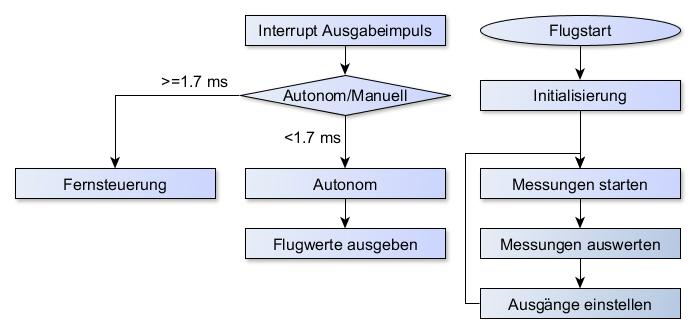
\includegraphics[width = \textwidth]{Bilder/Flussdiagramm}
    \par\end{centering}
    \caption{Flussdiagramm des Gesamtablaufs}
    \label{Flussdiragramm}
  \end{figure}

  Für die weiteren Programmteile wurden jeweils noch detailliertere Flussdiagramme erstellt.

%%%%%%%%%%%%%%%%%%%%%%%%%%%%%%%%%%%%%%%%%%%%%%%%%%%%%%%%%%%%%%%%%%%%%%%%%%%%%%%
\section{Navigation}

  \subsection{Technische Planung}

    \subsection*{Frames}
    Ein Frame entsteht bei jeder Messung der Pixy CMUcam5. Der Frame hat eine Breite von 319 und eine Höhe von 199 Pixel. Die Koordinate (0/0) befindet sich in der linken oberen Ecke.

    Bild 1 beschreibt den alten Frame, Bild 2 den aktuellen. Die Position des Objektes, beschreibt die zentralen x und y Positionen im Frame. Die Differenz entsteht aus den unterschiedlichen Positionen des Objektes im alten und neuem Frame. Das Objekt soll in den Bereich zwischen X\_MIN und X\_MAX, beziehungsweise Y\_MIN und Y\_MAX gelangen.

    % BILD VON LUCAS %

    \subsection*{Aileron}
    Anhand des aktuell getrackte Colorcodes wird die seitliche Position korrigiert. Solange sich der Hexacopter nicht im angegeben Bereich befindet, wird die Fluggeschwindigkeit in die jeweilige Richtung erhöht.

    \subsection*{Elevator}
    Durch den getrackten Colorcode, wird die Vorwärts- beziehungsweise Rückwärtsbewegung eingestellt. Die Position des Markers soll sich, wie bei der Bewegung nach Links und Rechts, in einem vorgegebenen Bereich befinden. 
    Das Kamerasystem trackt den ersten Marker, bis er sich im richtigen Bereich befindet und der zweite Marker erkannt wird, dieser wird ebenfalls verfolgt, danach kommt der dritte. Diese Routine läuft, bis der letzte Colorcode erreicht ist. Im Idealfall muss die Rückwärtsbewegung während des Fluges gar nicht durchgeführt werden. Die Rückwärtsbewegung findet ihre Anwendung nur, wenn der Hexacopter beim letzten Farbcode angekommen ist und über sein Ziel hinausfliegt, oder, wenn kein nächster Farbcode gefunden wird. Welcher Marker der Zielmarker ist, kann durch die Größe des Arrays, in dem die Marker gespeichert werden, herausgefunden werden. Dieses wird mit den Daten, die im Admin-Interface hinterlegt sind und im Endeffekt vom Wlan-Modul empfangen werden, befüllt.

    \subsection*{Rudder}
    Mithilfe der Rudder Funktion muss der Winkel auf die aktuelle Positionsmarkierung ausgerichtet werden. Dabei ist eine Ungenauigkeit von 5 Grad in beide Richtungen erlaubt.

    Für die Rotation werden die Grundlagen negativer binärer Zahlen benötigt.

    \begin{itemize}
    \item \textbf{Binäre Zahlen ohne Vorzeichen}\\
    0000 0000 = 0, 1111 1111 = 255
    \item \textbf{Binäre Zahlen mit Vorzeichen} - Ein Bit wird für das Vorzeichen verwendet. \\
    0000 0001 = 1 -> 1000 0001 = -1, \\
    0111 1111 = 127 -> 1111 1111 = -127
    \item \textbf{Einerkomplement} - Beim Invertieren aller Bits entsteht eine negative Zahl \\
    0000 0000 = "+0" -> 1111 1111 = "-0" \\
    0111 1111 = 127 -> 1000 0000 = -127
    \item \textbf{Zweierkomplement}\\
    0000 0001 = 1 -> 1111 1111 = -1 \\
    0000 0010 = 2 -> 1111 1110 = -2 \\
    0111 1111 = 127 -> 1000 0001 = -127
    \item \textbf{Bilden des Zweierkomplements}\\
    \textbf{Beispiel:} 0111 1111 = 127 \\
    Die binäre Zahl wird invertiert (1000 0000) und mit 1 addiert. \\
    Das Ergebins lautet: 1000 0001 = -127 \\
    \textbf{Beispiel:} 1001 1000 = -104 \\
    Die binäre Zahl wird invertiert (0110 0111) und mit 1 addiert. \\
    Das Ergebnis lautet: 0110 1000 = 104 \\
    \end{itemize}

    % Bild von Rotation %

    \subsection*{Throttle}
    Über den Ultraschallsensor erfährt der Hexacopter, wie hoch er fliegt. Beim Erreichen der maximalen Flughöhe, wird seine Antriebskraft gesenkt. Dadurch korrigiert er seine Höhe bei jedem Aufruf der Funktion und eine Änderung des Gewichts, kann ausgeglichen werden. Der entnommene Cupcake und die damit verbundene Gewichtsveränderung stellt daher kein Problem dar.

  \subsection{Umsetzung}

    \subsubsection{Vergleichen der Frames}
    Für den Vergleich des aktuellen Frames mit dem letzten Frame, werden zwei \glslink{Struktur}{Strukturen} verwendet, die über folgende Mitglieder verfügt. \cite{Structs}
    \begin{itemize}
      \item \textbf{num} ist die ID des getrackten Colorcodes, er besteht aus einer zweistelligen Zahl.
      \item \textbf{pos\_x} ist die X-Position des Colorcodes. Der Wert bezieht sich auf das Zentrum des Objektes.
      \item \textbf{pos\_y} ist die Y-Position des Colorcodes. Der Wert bezieht sich auf das Zentrum des Objektes.
      \item \textbf{height} ist die, vom Ultraschall übergebene Höhe.
      \item \textbf{angle} ist die Rotation des Colorcodes. Da er zweifarbig ist, kann die PIXY CMUcam5 die Rotation des Objektes feststellen.
    \end{itemize}

    Zuerst wird die ID des Colorcodes verglichen, um herauszufinden, ob das Farbobjekt das selbe ist, wie im letzten Frame.
    Sollte dies der Fall sein, werden die Koordinaten x und y und die Rotation mit den Werten der älteren Struktur verglichen und in einer weiteren Strunktur gespeichert. Dieses wird bei den folgenden Funktionen verwendet, um anhand der Änderung zwischen zwei Frames zu überprüfen, ob der Hexacopter die richtige Geschwindigkeit hat.

    \subsubsection{Aileron, Elevator und Rudder anhand der Kameradaten}
    Durch die PIXY CMUcam5 kann die Position des Hexacopters, relativ zu einem Colorcode, festgestellt werden. Gegebenenfalls werden anschließend die Flugparameter verändert.

    \begin{figure} [tbh]
      \begin{centering}
        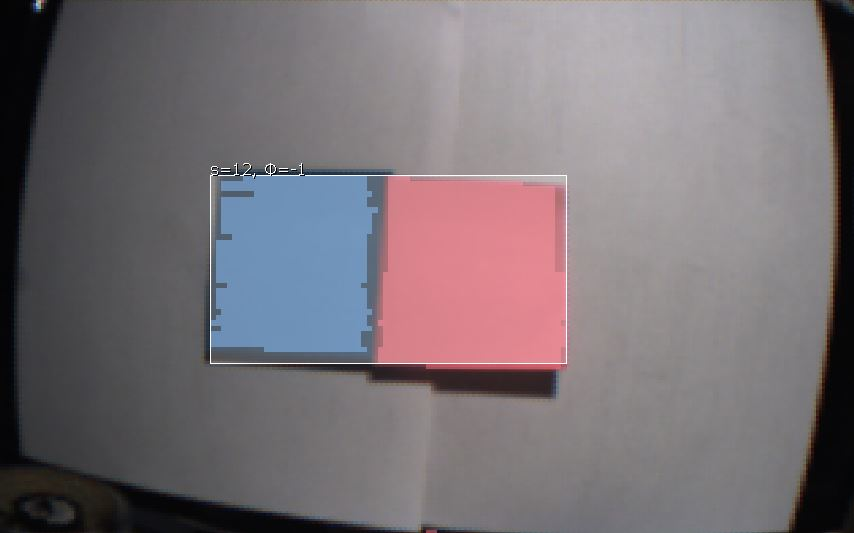
\includegraphics[width = \textwidth]{Bilder/Farbcode_erkannt}
      \par\end{centering}
      \caption{Ein erkannter Farbcode}
      \label{Farbcode_erkannt}
    \end{figure}
    Die Position wird anhand solcher Farbcodes erkannt, im Tischkonzept ist hinterlegt in welcher Reihenfolge der Hexacopter die Farbcodes suchen muss.
    Er fliegt anschließend so lange, bis er über dem aktuellen Farbcode ist, dieser also mittig im Bild ist und sucht darauf den nächsten.

    \subsubsection{Überprüfen von Aileron}
    Beim Vergleichen von Aileron wird die Veränderung an der x-Achse überprüft.

    Durch diese Funktion soll der Hexacopter mithilfe der Pixy-Daten, den Colorcode in der Mitte des Frames plazieren. An der x-Achse sind Werte zwischen 150 und 170 optimal. Der übergebene Wert ist dabei der Mittelpunkt des Colorcodes.
    Sollte die Pixycam keinen Wert in diesem Bereich erfassen, kann sie durch eine weitere Funktion namens ActAileron, welche die Änderungsrate an den Flightcontroller weitergibt, die Position an der x-Achse korrigieren.
    Um herauszufinden, ob der Mittelpunkt unter oder über dem optimalen Wert liegt, also der Hexacopter zu weit links oder rechts vom Objekt fliegt, gibt es für beide Fälle eine Abfrage.
    Um den Aileron Wert entgültig zu setzen, müssen nach der Überprüfung, ob der übergebene Wert an der x-Achse 170 überschreitet beziehungsweise 150 unterschreitet, folgende Zustände kontrolliert werden.
    Zunächst muss der Hexacopter über die Pixycam herausfinden, ob er sich bereits in die richtige Richtung bewegt. Dafür werden die beiden Frames miteinander verglichen. Wenn der Wert zu hoch ist, muss der x-Wert im alten Frame größer als im neuen sein. Sollte er zu niedrig sein, muss der Wert im neuen Frame höher sein.
    Anderenfalls fliegt der Hexacopter auf die falsche Seite. Die Firmware reagiert darauf mit der Änderung der Pulszeit am Aileron-Pin.
    Bei der Bewegung in die richtige Richtung wird der Wert so lange in diese gesteuert, bis sich die Geschwindigkeit, gemessen in den veränderten Pixel zwischen zwei Frames, zwischen zwei konstanten Werten befindet.

    \subsubsection{Überprüfen von Elevator}
    Elevator, die Bewegung an der y-Achse, also die Bewegung nach vorne und nach hinten, funktioniert nach dem selben Prinzip wie Aileron.

    Zuerst wird kontrolliert, ob sich der Farbcode im gewünschten Bereich befindet, in diesem Fall zwischen 90 und 110.
    Sollte der Mittelpunkt an der y-Achse nicht in diesem Bereich liegen, fliegt der Hexacopter nach vorne beziehungsweise zurück.
    Da die Route aus mehreren Farbcodes besteht, richtet sich der Hexacopter, sobald der Colorcode im Bereich zwischen 90 und 100 liegt, nach dem Objekt, das sich am nächsten zum Nullpunkt der y-Achse befindet. Somit probiert er die Position zentriert über dem Farbobjekt zu optimieren, bis er das nächste Farbobjekt erkennt und trackt. Das alte Objekt ist nun unwichtig, der Hexacopter bezieht sich auf das vordere Farbobjekt.

    Wie bei der Überprüfung von Aileron, gibt es auch hier zwei konstante Werte, zwischen denen sich die Geschwindigkeit befinden soll, solange die Position optimiert wird.

    \subsubsection{Überprüfen von Rudder}
    Rudder beschreibt die Rotation um seine eigene Hochachse. Dafür wird zunächst unterschieden, ob sich der Hexacopter am Hin- oder Rückflug befindet, da die Rotation der Colorcodes beim Rückflug um 180 Grad gedreht werden muss.

    Die optimale Rotation befindet sich beim Hinflug zwischen -5 und 5 Grad.
    Bei einem zu niedrigen oder zu hohen Wert wird kontrolliert, ob sich der Hexacopter bereits in die richtige Richtung dreht.
    Sollte dies nicht der Fall sein, wird die Änderungsrate an die dazugehörige Funktion geschickt, die dem Flightcontroller die Information zur Beschleunigung gibt.
    Ansonsten wird die Veränderung der Pixel zweier Frames verglichen, wenn sie sich im gewünschten Bereich befindet, wird der Wert nicht geändert, bei einem zu hohen Wert, wird die Rotationsgeschwindigkeit gesenkt, ansonsten erhöht.

    Beim Rückflug soll die Rotation des Colorcodes größer als 175 oder kleiner als -175 sein.

    \subsubsection{Throttle anhand des Ultraschallsensors}
    Der Hexacopter steht auf einer Landeplattform in seiner Base. Unter ihm ist ein Farbcode, den er so lange fokusiert, bis er den nächsten Farbcode trackt. Den zweiten Farbcode kann er erst scannen, wenn er hoch genug fliegt um an der Tischkante vorbei, den nächsten Farbcode zu scannen.

    Beim Starten fliegt er vertikal nach oben, bis er den zweiten Farbcode erkennt. Um beim Start nicht abzudriften, beschleunigt er, solange er sich unter einer Höhe von $\SI{50}{\centi\metre}$ befindet, mit einer hohen Änderungsrate. Ab dieser Höhe beschleunigt er mit einer geringeren Erhöhung der Änderungsrate, bis er die $\SI{80}{\centi\metre}$-Grenze erreicht hat.
    zwischen $\SI{80}{\centi\metre}$ und $\SI{120}{\centi\metre}$ bleibt die Beschleunigung gleich, das führt jedoch dazu, dass der Hexacopter den oberen Rand von $\SI{120}{\centi\metre}$ erreichen wird, da er bis jetzt nicht gebremst wird. Sobald er über $\SI{120}{\centi\metre}$ kommt, wird die Beschleunigung reduziert. Der Hexacopter pendelt sich zwischen $\SI{80}{\centi\metre}$ und $\SI{120}{\centi\metre}$ ein.

    Nun wird berechnet, ob er sich noch über dem Tisch oder schon über dem Boden befindet. Dies stellt er fest, wenn zwei hintereinanderliegende Messungen einen Höhenunterschied von $\SI{50}{\centi\metre}$ aufweisen. Die zweite Messung ist erforderlich, um mögliche Fehlmessungen auszuschließen.

    Wenn er nun über dem Boden fliegt, beträgt seine minimale Höhe $\SI{180}{\centi\metre}$ und seine maximale Höhe $\SI{220}{\centi\metre}$.
    Der Hexacopter beschleunigt nach dem selben Prinzip, wie über einem Tisch. Unter $\SI{100}{\centi\metre}$ ändert er seine Beschleunigung mit einem hohen Wert. Bis $\SI{180}{\centi\metre}$ beschleunigt er mit einer niedrigeren Änderungsrate. Sollte der Hexacopter über $\SI{220}{\centi\metre}$ fliegen, wird die Beschleunigung durch eine negative Änderungsrate gesenkt.

    Der Hexacopter fliegt mit diesen Werten, bis er den vorletzten Farbcode erreicht hat. Da die Farbcodes in einem Array abgespeichert werden, ist die Anzahl der darin gespeicherten Farbcodes bekannt.

    Beim letzten Farbcode angekommen, also dem am Tisch liegenden Farbcode, wird ebenfalls wieder durch die Kontrolle von zwei Werten, die sich um $\SI{50}{\centi\metre}$ von der vorigen Messung unterscheiden müssen, analysiert, wann sich der Hexacopter über dem Tisch befindet. Sobald dies der Fall ist, landet er, indem er die Beschleunigung mit einer negativen Änderungsrate verlangsamt. Dabei muss er sich, zwischen einer vom System vorgegebenen Mindest- und Maximalgeschwindigkeit, befinden.

    Nach der Landung wird die Routeninformation umgekehrt, der erste Colorcode wird zum letzten, der zweite zum vorletzten und so weiter. Außerdem muss die Rotation der Farbcodes beim Rückflug um 180 Grad gedreht sein, dafür wird die Richtung als Rückflug abgespeichert. Sollte sich der Hexacopter wieder in der Base befinden, wird die Variable wieder als Hinflug gespeichert.

    Damit genügend Zeit für das herunternehmen des Cupcakes ist, verweilt der Hexacopter eine halbe Minute am Tisch, bevor er seinen Rückflug antritt.

    \subsubsection{Speichern der alten Daten}
    Die alten Daten werden gespeichert, um die Differenzen von zwei Frames zu errechnen. Der Frame mit Index 0, ist der aktuelle Frame, der Frame mit dem Index 1, der alte. Bei jedem Durchlauf, werden die Werte aktualisiert.

    \subsubsection{Ausgabe der Steuersignal}
    Autor: Lucas Ullrich\\
    Nachdem die Steuersignale berechnet und korrigiert wurden, müssen diese an den Hexacopter ausgegeben werden. Dies muss periodisch alle $\SI{20}{\milli\second}$ geschehen.
    Der Flightcontroller erkennt jeweils die einzelnen Impulse und steuert die Rotoren entsprechend an.

    Diese Impulse werden interruptgesteuert ausgegeben, der Interrupt wird von dem Gear-Pin erzeugt, welcher gleichzeitig für den Flugmodus verantwortlich ist.

    \lstset{language = c}
    \begin{lstlisting}
interrupt void Isr() {
  if(CCP1IF == 1) {
    CCP1IF = 0;
    T1CONbits.TMR1ON = 0;
    SignalOut();
    NOP();
  }
  if(TMR3GIF == 1) {
    TMR3GIF = 0;
    ModeCheck();
    SignalOut();    /* initial call after remaining break to 20 ms
                     * starts with Aileron (needs to be set in last
                     * case statement, case 0) following delays will
                     * be processed by the previous routine */
    pulsecounter++;
  }
}

void SignalOut(void) {
  switch(pin_out) {
    case 'A': {
      A = 1;
      Delay(a_actors[0].aile);
      pin_out = 'E';
      break;
    }case 'E': {
      A = 0;
      E = 1;
      Delay(a_actors[0].elev);
      pin_out = 'T';
      break;
    }
    \end{lstlisting}
    Die weiteren Signale (Throttle und Rudder) werden auf die gleiche Weise ausgegeben.
    Die Delay-Funktion stellt die Compare-Einheit so ein, dass nach der gewünschten Pulsdauer des Ausgangs ein Interrupt hervorgerufen wird.

%%%%%%%%%%%%%%%%%%%%%%%%%%%%%%%%%%%%%%%%%%%%%%%%%%%%%%%%%%%%%%%%%%%%%%%%%%%%%%%
%\section{Objekterkennung}

  %\subsection{Technische Planung}

  %\subsection{Umsetzung}

  %\subsection{Herausforderungen und Lösungen}

%%%%%%%%%%%%%%%%%%%%%%%%%%%%%%%%%%%%%%%%%%%%%%%%%%%%%%%%%%%%%%%%%%%%%%%%%%%%%%%
\section{Sicherheit}

  \subsection{Technische Planung}

Sicherheitskonzepte

Beim Konzept Sicherheitsmaßnahmen geht es grundsätzlich um die Sicherheit von Mensch, Umgebung und dem Multicopter selbst. Hier werden mögliche Fehler mit Anlehnung an FMEA ("Fehlermöglichkeits- und -einflussanalyse" / "Auswirkungsanalyse") analysiert. Dieses Konzept ist ein rein schriftliches Konzept.

  \subsection{Umsetzung}

    Legende:
    \begin{itemize}
    \item A: Auftreten
    \item B: Bedeutung
    \item E: Entdeckung
    \item RPZ: Risiko-Prioritätszahl = A * B * E
    \end{itemize}

    Die Werte beziehen sich auf den Fehler, die obere Analyse beschreibt das Auftreten, die Bedeutung und die Entdeckung vor den Maßnahmen, die unteren nach den Maßnahmen.

%\begin{table}[H]
%\centering
\begin{longtable}{|p{0.4cm}|p{3.0cm}|p{3.1cm}|p{3.1cm}|p{0.4cm}|p{0.4cm}|p{0.4cm}|p{0.8cm}|}

\hline \#   & Bezeichnung                                                                                               & Fehler                                                                                                                & Beschreibung                                                                                                                    & A   & B   & E   & RPZ \\
 1          & Mensch in unmittelbarer Nähe                                                                              & Mensch wird verletzt, da Hexacopter nicht ausweicht                                                                   & Eine Person steht auf dem Weg und wird vom Hexacopter als Hindernis erkannt                                                     & 5   & 10  & 10  & 500 \\
\hline -    & Vermeidung                                                                                                & Maßnahme nach Eintritt                                                                                                & Mögliche Softwarelösung                                                                                                         & A   & B   & E   & RPZ \\
 -          & Wege absperren, Menschen darauf hinweisen, sich nicht in unmittelbarer Nähe des Hexacopters aufzuhalten.  & Hexacopter landet auf der Stelle um die Sicherheit der Person zu gewährleisten.                                       & Durch 2 Ultraschallsensoren, die vorne am Hexacopter angebracht sind, werden Menschen erkannt, er landet daraufhin.             & 2   & 10  & 5   & 100 \\\hline

\hline \#   & Bezeichnung                                                                                               & Fehler                                                                                                                & Beschreibung                                                                                                                    & A   & B   & E   & RPZ \\
 2          & Ein unbewegliches Hindernis befindet sich in unmittelbarer Nähe.                                          & Hexacopter fliegt gegen ein unbewegliches Hindernis und stürzt ab.                                                    & Eine Wand oder ein ähnliches unbewegliches Hindernis befindet sich in unmittelbarer Nähe.                                       & 5   & 7   & 9   & 315 \\
\hline -    & Vermeidung                                                                                                & Maßnahme nach Eintritt                                                                                                & Mögliche Softwarelösung                                                                                                         & A   & B   & E   & RPZ \\
 -          & Farbcodes werden nicht in der Nähe von unbeweglichen Hindernissen platziert.                              & Der Hexacopter landet, da er nicht zwischen Mensch, beweglichen und unbeweglichen Hindernissen unterscheiden kann.    & Der Hexacopter darf nur über Farbcodes fliegen, dadurch wird vermieden, dass der Hexacopter in die Nähe dieser Objekte kommt.   & 1   & 7   & 5   & 35  \\\hline

\hline \#   & Bezeichnung                                                                                               & Fehler                                                                                                                & Beschreibung                                                                                                                    & A   & B   & E   & RPZ \\
 3          & Bewegliches Hindernis wird erkannt                                                                        & Hexacopter fliegt gegen ein Hindernis und stürzt ab                                                                   & Eine Hindernis wird erkannt.                                                                                                    & 3   & 6   & 10  & 180 \\
\hline -    & Vermeidung                                                                                                & Maßnahme nach Eintritt                                                                                                & Mögliche Softwarelösung                                                                                                         & A   & B   & E   & RPZ \\
 -          & Bewegliche Hindernisse werden wenn möglich aus dem Weg geräumt.                                           & Hexacopter probiert dem Hindernis auszuweichen und seinen Weg weiter zu meistern.                                     & Durch 2 Ultraschallsensoren, die vorne am Hexacopter angebracht sind, werden Hindernisse erkannt, er landet daraufhin           & 2   & 6   & 5   & 60  \\\hline

\hline \#   & Bezeichnung                                                                                               & Fehler                                                                                                                & Beschreibung                                                                                                                    & A   & B   & E   & RPZ \\
 4          & Hände in der Nähe von den Propellern                                                                      & Person hat seine Hände beim fliegenden Hexacopter und verletzt sich                                                   & Eine Person greift in die Propeller.                                                                                            & 7   & 10  & 10  & 700 \\
\hline -    & Vermeidung                                                                                                & Maßnahme nach Eintritt                                                                                                & Mögliche Softwarelösung                                                                                                         & A   & B   & E   & RPZ \\
 -          & Hexacopter wartet lang genug, dass man den Cupcake runternehmen kann. Propellerschutz ist angebracht.     & Hexacopter gibt über Display / LED / Ton aus, dass er wegfliegt.                                                      & Display / LED / Ton werden programmiert um Menschen beim Start zu warnen.                                                       & 1   & 10  & 5   & 50  \\\hline
 \caption{Fehlt noch}
\end{longtable}
%\end{table}


%%%%%%%%%%%%%%%%%%%%%%%%%%%%%%%%%%%%%%%%%%%%%%%%%%%%%%%%%%%%%%%%%%%%%%%%%%%%%%%
\section{Systemausfall}

Das Konzept Systemausfall beschreibt die Maßnahmen, wenn der Hexacopter seine Anforderungen nicht erfüllen kann. Dieses Konzept ist rein schriftlich entwickelt.

  \subsection{Technische Planung}

  Mögliche Ursachen: \cite{tech_def}
  \begin{itemize}
  \item Materialermüdung
  \item Programmfehler (eingespeiste Daten, Programmablauffehler)
  \item menschlicher Fehler
  \item falsche Montage
  \item fehlender elektrischer Kontakt
  \item unzureichende oder fehlende Energieversorgung
  \item Fehler in der Datenverarbeitung; beispielsweise Datenübertragung, Informationsverlust, Rechenfehler
  \end{itemize}


  \subsection{Umsetzung}
  Mit einem Stern gekennzeichnete Fehler, sind in der Firmware berücksichtigt.

\begin{table}[H]
\centering
\begin{tabular}{|p{7cm}|p{7cm}|}
\hline Fehler & Lösung\\\hline
\hline Akku schwach & Fail Safe, eventuell sofort landen\\
\hline Akku explodiert: Lithium Ionen Akkus können explodieren & Vor dem Flug kontrollieren, Feuerlöscher bereitstellen\\
\hline Copter findet keine Farbobjekte mehr & Position Hold, nach einer Zeit: Landen\\
\hline Copter findet falsche Farbobjekte & Position Hold, nach einer Zeit: Landen \\
\hline Ausfall von Aktoren (Propeller, bzw. Motoren blockiert/ …) &  Wenn es möglich ist: Landen\\
\hline Copter fliegt in die falsche Richtung * & Da Colorcodes aus 2 Farben bestehen, kann die Rotation des Objektes bestimmt und korrigiert werden. \\
\hline Hexacopter ist zu hoch / verliert an Höhe * & Durch die Daten des Ultraschallsensors, kann die Höhe korrigiert werden.\\
\hline Ausfall von Sensoren (Pixy / Ultraschall / …) & Fehlermeldung, Manueller Flug\\
\hline Hackerangriff & Durch den WLAN Standard (wpa2) ist die Übertragung sicher genug\\
\hline Funkstörung bei manuellem Flug & Pilot muss verstehen, in welchem Frequenzband die Fernsteuerung arbeitet, Störquellen vermeiden und abschalten (sonstiges WLAN, Bluetooth, andere Fernsteuerungen im Umfeld) -> saubere Vorbereitung - Analyse von möglichen Störquellen\\
\end{tabular}
\caption{Fehlt noch}
\end{table}

\subsection*{Beispiele für Lösungen}
\begin{itemize}
\item \textbf{Landen:} sofort auf der Stelle landen
\item \textbf{Position hold:} in der Luft stehen bleiben – Option auf manuelle Steuerung umstellen
\item \textbf{Fail Safe:} zurück zur Base fliegen und Flug abbrechen
\item \textbf{Manuell fliegen:} auf manuelle Fernsteuerung umschalten
\item \textbf{Fehlermeldung:} Fehlermeldung wird über Display oder blinkende LEDs ausgegeben. Fehler wird an Server gesendet
\end{itemize}

\subsection*{Was passiert nach einem Systemausfall?}
Wenn der Hexacopter seinen Fehler selbst korrigieren kann, fliegt er seine Route weiter.
Anderenfalls geht der Hexacopter, sobald er gelandet ist oder manuell gesteuert wurde, davon aus, beim nächsten Start in seiner Base zu stehen. Der Cupcake wird wieder in der Bestellliste angezeigt und muss erneut ausgeliefert werden. Je nach Fehler, wird ein Code über den Display ausgegeben, der bei der Fehlersuche helfen soll.


% !TEX root = diplomarbeit.tex
\chapter{Kommunikation Applikation und Hexacopter}
\renewcommand{\kapitelautor}{Autor: Katharina Joksch, Lucas Ullrich}
Um zwischen dem Hexacopter und dem Server eine Verbindung herzustellen wird eine Kommunikationsschnittstelle benötigt. Diese muss Drahtlos arbeiten und einen größeren Bereich
abdecken. Über diese werden anschließend die diversen Daten übertragen, dazu zählen \zB die Route, \bzw der Name des Gastes.

%%%%%%%%%%%%%%%%%%%%%%%%%%%%%%%%%%%%%%%%%%%%%%%%%%%%%%%%%%%%%%%%%%%%%%%%%%%%%%%
\section{Allgemeine technische Planung}
In der Planung wurde eine unkomplizierte und verlässliche Lösung für beide Kommunikationspartner gesucht. Da Bluetooth kaum noch standardmäßig verbaut wird hier wiederum
Serverseitig eine externe Hardware benötigt, um dies zu vermeiden wurde WLAN ins Auge gefasst.

WLAN stellte sich folglich als ideale Schnittstelle heraus,
es gibt die Möglichkeit zu Handover in sehr großen Bereichen, es ist nach einmaligem Setup vergleichsweise unkompliziert und es bietet diverse Möglichkeiten um festzustellen
ob die Verbindung noch aufrecht ist.

%%%%%%%%%%%%%%%%%%%%%%%%%%%%%%%%%%%%%%%%%%%%%%%%%%%%%%%%%%%%%%%%%%%%%%%%%%%%%%%
\section{Schnittstelle Hexacopter}
Seitens des Hexacopters wird ein zusätzliches Modul benötigt, dieses muss über eine der Schnittstellen des Mikrocontrollers ansprechbar sein.

  \subsection{Technische Planung}
  Bei der Planung wurde darauf geachtet ein WLAN-Modul zu wählen welches bekannter maßen funktioniert \bzw ein entsprechender Support zur Verfügung steht.
  So fiel die Wahl auf das WLAN-Modul RN171, vertrieben durch Microchip, hergestellt von Roving Networks.

  Das gewählte WLAN-Modul wird über eine UART-Schnittstelle angesteuert und verfügt über einige frei konfigurierbare Pins, diese werden schließlich zum Überwachen der
  Verbindung verwendet.

  \subsection{Umsetzung}
  Bei der Umsetzung stand für die anfänglichen Tests ein Evaluation-Kit zur Verfügung. Dieses kann ohne weitere Hardware direkt über ein USB-Kabel mit einem PC verbunden werden.
  So ist es möglich die nötigen Konfigurationen des Moduls auszutesten bevor dieses in der Hardware implementiert wird.

  \begin{figure}[H]
    \begin{centering}
      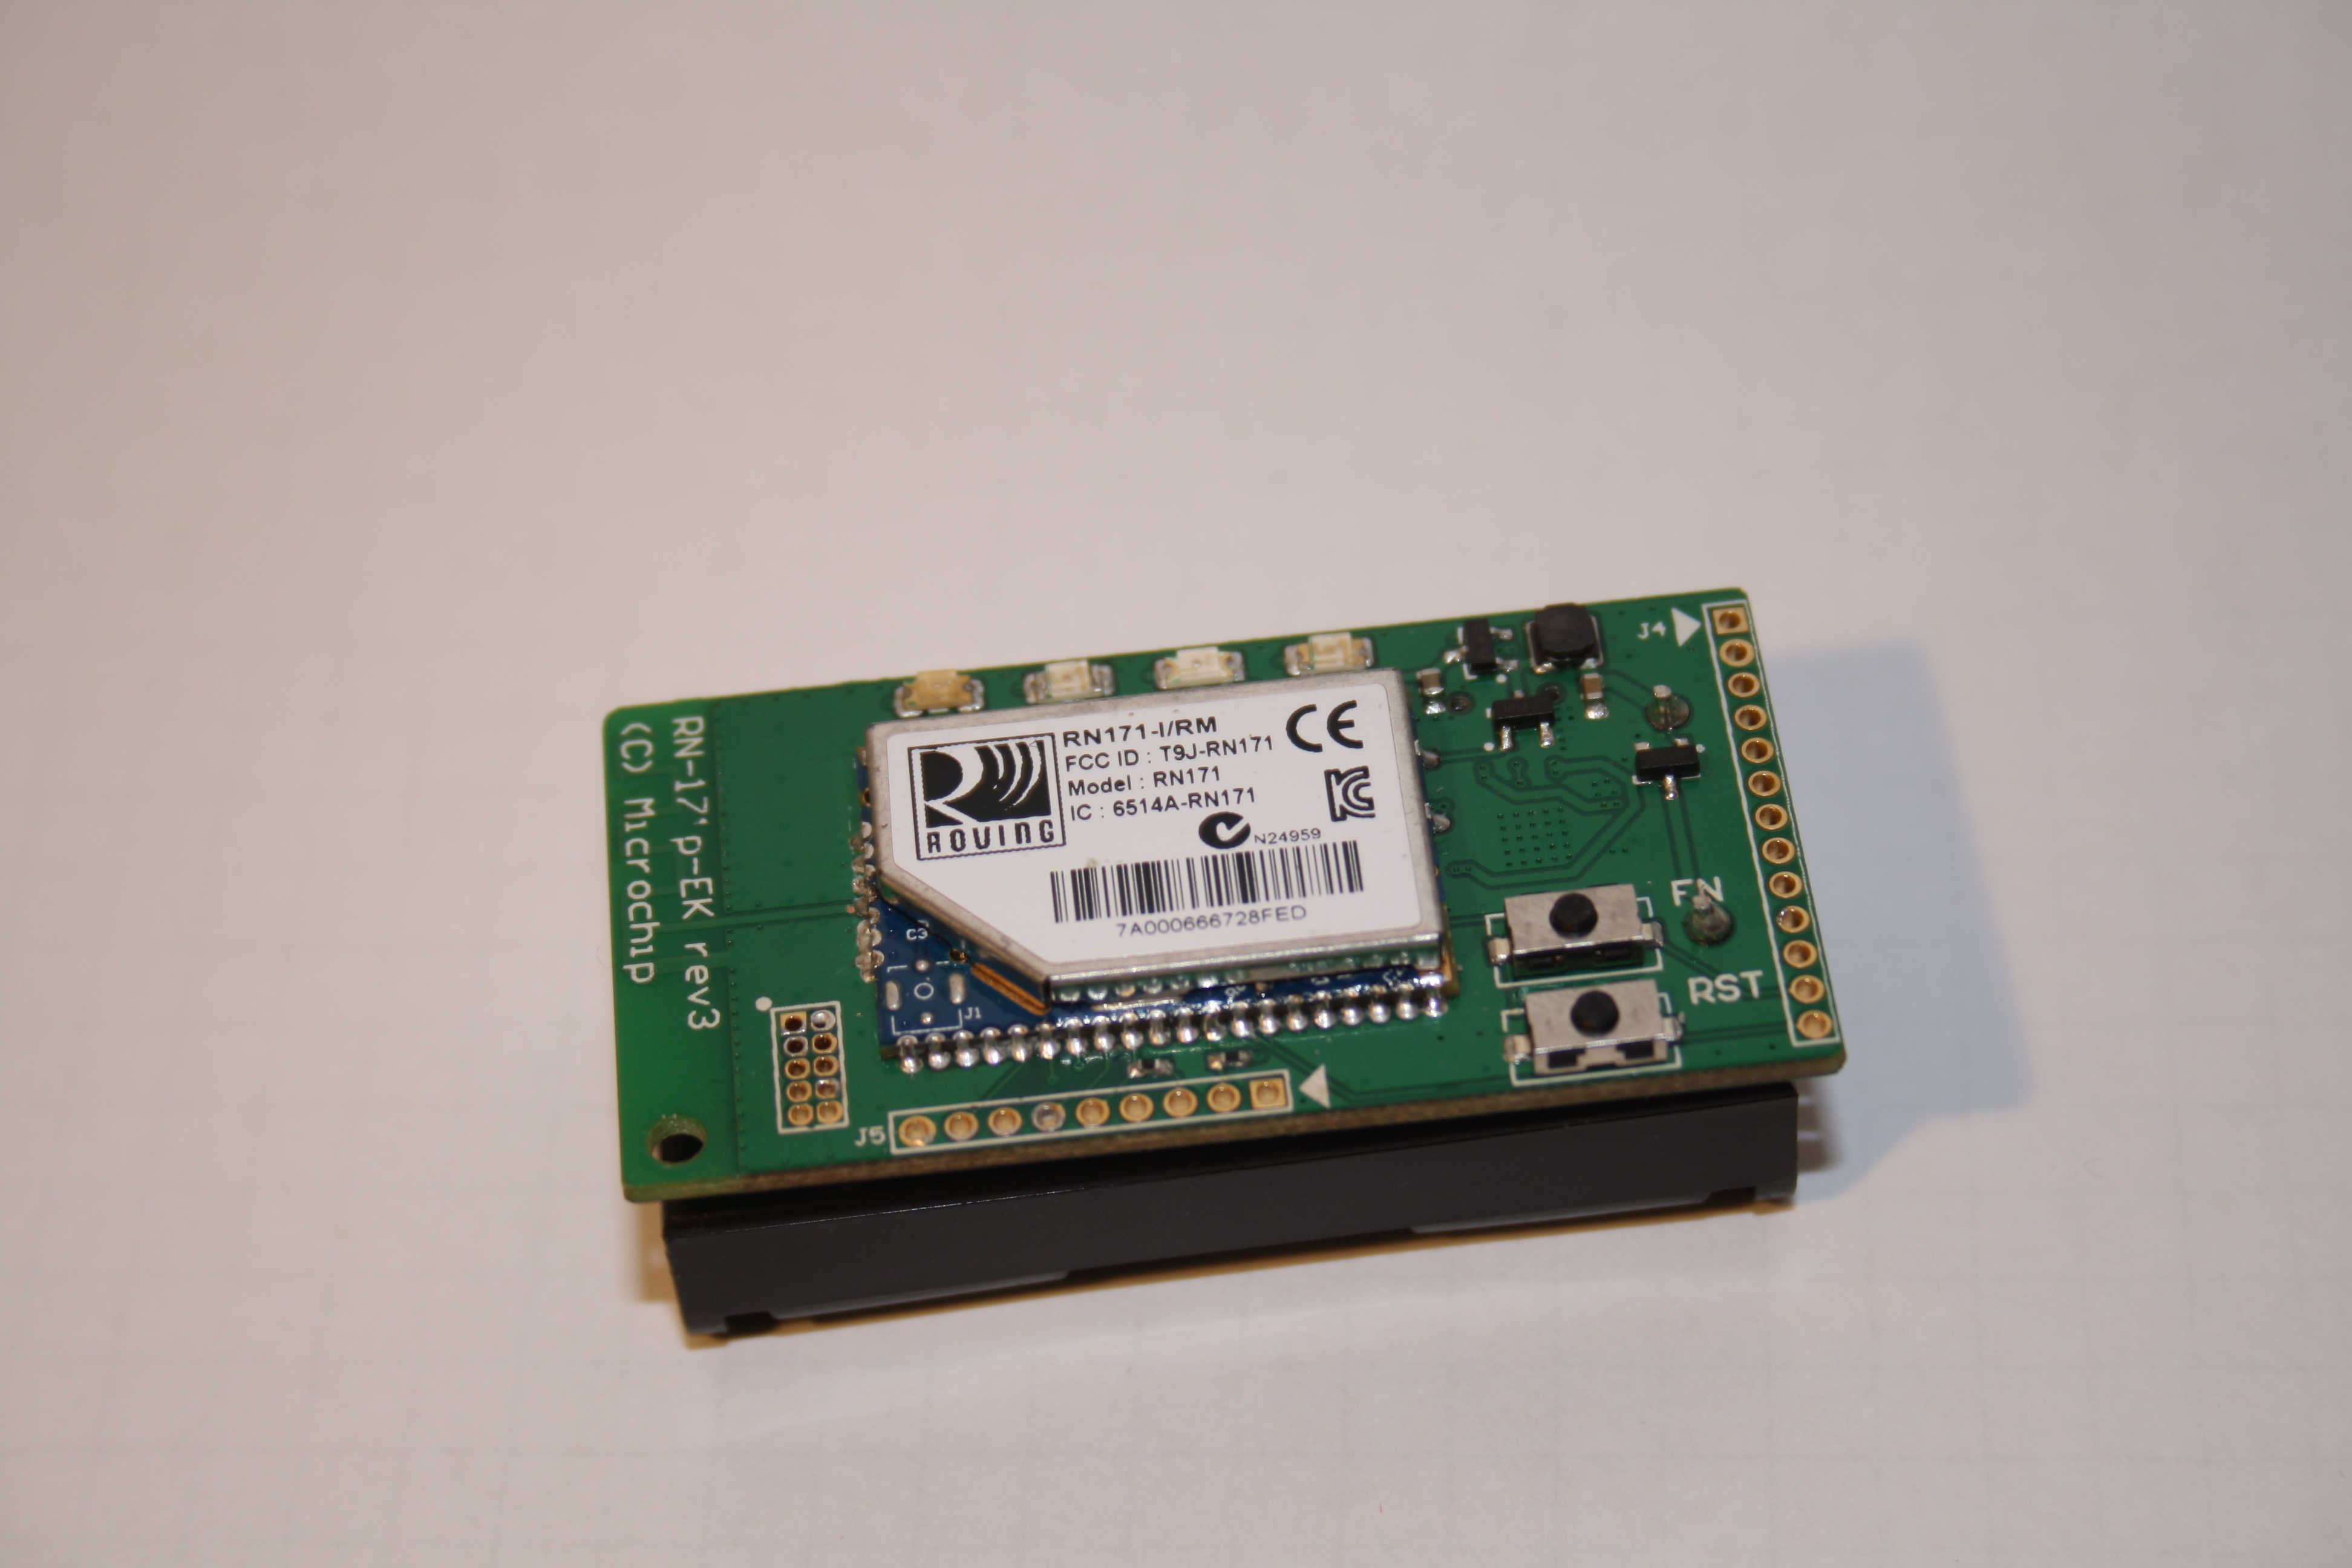
\includegraphics[width = 0.6\textwidth]{Bilder/RN171_EK}
    \par\end{centering}
    \caption[RN171 Evaluation-Kit]{RN171 Evaluation-Kit\cite{RN171_EK_source}}
    \label{RN171_EK}
  \end{figure}

  Um das WLAN-Modul so einzustellen, dass es sich Pin-gesteuert mit einem Host verbindet sind einige Schritte notwendig:
  \begin{itemize}
    \item \textbf{\$\$\$}\\
    Öffnet den Commandmode, nun können die Einstellungen vorgenommen werden
    \item \textbf{set wlan ssid <network\_name>}\\
    Deklariert den Netzwerknamen
    \item \textbf{set wlan phrase <network\_passphrase>}\\
    Deklariert das Passwort mit dem das Netzwerk gesichert ist
    \item \textbf{set ip host <host\_ip-address>}\\
    Deklariert die IP-Adresse des Empfängers
    \item \textbf{set ip remote <host\_portnumber>}\\
    Deklariert den Port auf dem der Empfänger die Daten empfangen soll
    \item \textbf{set sys iofunc 0x70}\\
    Durch diese Einstellung kann das WLAN-Modul über die Pins gesteuert werden
    \item \textbf{set wlan join 1}\\
    Stellt das WLAN-Modul auf automatisches Verbinden mit dem angegebenen Netzwerk ein
    \item \textbf{set ip protocol 4}\\
    Stellt das WLAN-Modul auf eine TCP/IP-Verbindung ein bei der nur Daten vom gespeicherten Host akzeptiert werden
    \item \textbf{set uart baud <desired-baudrate>}\\
    Stellt die Baudrate des WLAN-Moduls ein, Standard ist 9600
    \item \textbf{save}\\
    Speichert die Parameter in den Standardeinstellungen die nach einem Neustart geladen werden
    \item \textbf{reboot}\\
    Erzeugt einen Neustart bei dem die Standardeinstellungen geladen werden
  \end{itemize}
  Nachdem das WLAN-Modul auf die nötigen Parameter eingestellt ist, kann es direkt mit dem Mirkocontroller verbunden werden, die Verbidnung kann über einzelne Pins kontrolliert
  werden.

  \subsection{Herausforderungen und Lösungen}
  Eine Herausforderung stellte die Frage dar wie genau die Verbindung hergstellt wird. Das Datenblatt des WLAN-Moduls mit über 100 Seiten bietet viele potentielle Möglichkeiten.
  Die erste Wahl fiel auf das Auslesen einer Website, auf den ersten Anblick funktionierte das auch, jedoch musste festgestellt werden, dass unabhängig von der Website sehr ähnliche
  Daten verarbeitet werden, jedoch nicht der eigentliche Inhalt der Website sondern Providerinformationen.

  Die zweite Wahl fiel auf eine TCP/IP Verbindung, lediglich die genaue Umsetzung dieser ließ viele Möglichkeiten offen. Einerseits besteht die Möglichkeit eine Verbindung direkt
  über die Eingabe "open" im Commandmode zu öffnen, andererseits jedoch auch über die Pins als auch automatische Timeouts.

  Aufgrund der Einfachheit und vollen Kontrolle viel die Wahl auf die Ansteuerung über die Pins.
  Dazu stehen 3 unterschiedliche Pins zur Verfügung:
  \begin{itemize}
    \item \textbf{Associated}\\
    Mit einem Netzwerk verbunden
    \item \textbf{Open TCP connection}\\
    Die Verbidnung zum Host herstellen
    \item \textbf{Connected}\\
    Die Verbindung zum Host ist hergestellt
  \end{itemize}
  Die Statusinformationen Associated als auch Connected werden von dem WLAN-Modul geliefert, die Anweisung eine Verbindung herzustellen von dem Mirkocontroller.

%%%%%%%%%%%%%%%%%%%%%%%%%%%%%%%%%%%%%%%%%%%%%%%%%%%%%%%%%%%%%%%%%%%%%%%%%%%%%%%
\section{Schnittstelle Applikation}

  \subsection{Technische Planung}
  
      \subsubsection{Eclipse}
    
Eclipse ist eine freie Entwicklungsumgebung für Programme und wurde von der Eclipse Foundation entwickelt. Das Programm kann verwendet werden, um in mehreren Programmiersprachen Software zu entwicklen. Besonders gut geeignet ist Eclipse für die Entwicklung von Java-Programmen, da es sowohl Auto-Completion ermöglicht als auch Syntax- Highlighting.

	   \subsubsection{JDBC}

Die Java Datenbankschnittstelle JDBC ist ein Industriestandard für datenbankunabhängige Verbindungen zwischen Java Programmen, SQL Datenbanken und sämtlichen anderen tabellenbasierten Datenbankmodellen. Zu den Aufgaben von JDBC gehört es, Datenbankverbindungen aufzubauen und diese zu verwalten. Außerdem kann JDBC  SQL-Anfragen an die Datenbank weiterleiten, Ergebnisse in eine für Java nutzbare Form umwandeln und diese dem Programm zur Verfügung stellen.

	   \subsubsection{Zusammenspiel mit der Applikation und dem WLAN-Modul}
Das Java-Programm und die Applikation kommunizieren nur indirekt miteinander, da beide nur auf die Datenbank zugreifen um deren Inhalt zu überprüfen und Einträge updaten beziehungsweise erstellen.
Mit dem WLAN-Modul wird hingegen auf direktem Weg kommuniziert. Dieses wird nämlich als Thread etabliert und direkt in den Javaklassen verwaltet.
			\begin{figure}[H]
			\begin{centering}
			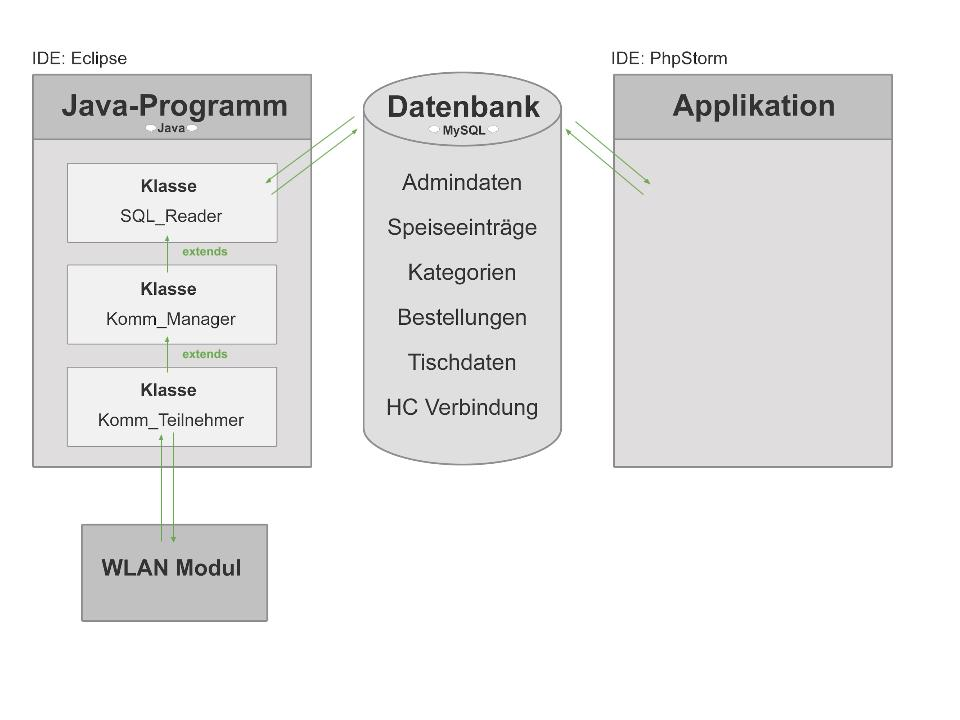
\includegraphics[width = 1\textwidth]{Bilder/Jok_zusammenspiel_java.jpg}
			\par\end{centering}
			\caption{neue MockUps - Admininterface}
			\label{neue MockUps - Admininterface}
			\end{figure}
  \subsection{Umsetzung}
Für die Umsetzung des Javaprogramms wurden drei verschiedene Klassen erstellt:
\begin{itemize}
    \item \textbf{SQL Reader}\\
Diese Klasse wurde dazu programmiert, alle Datenbankzugriffe zu regeln.
Um den Zugriff auf Datenbanken zu bewerkstelligen wurde JDBC verwendet. 
Damit das Programm mit JDBC arbeiten kann muss man es erst einmal von Oracle downloaden und anschließend mit einem Rechtsklick auf das Javaprojekt unter dem Menüpunkt "Properties" als Bibliothek angeben.
Wie auch bei Doctrine müssen der Datenbank Host, der Datenbank Port und die Benutzerdaten angegeben werden, damit die Verbindung hergestellt werden kann.
Als Treiber wird hier jedoch statt MySQL auf JDBC verwiesen. 
Um die Verbindung herzustellen wurde auf die Funktion DriverManager.getConnection() aufgerufen. Als Parameter musste ihr der Pfad zur Datenbank und die Benutzerdaten mitgeschickt werden.
\\
Damit die Tischdaten angezeigt werden konnten, wurde die "showTischdaten()"-Funktion erstellt. Um die ID, die Tischroute und die Tischnummer zu erhalten musste jeweils ein SQL-Statement, welches die Tischdaten ausliest, denen die Bestellung zugewiesen ist, verfasst werden, welches anschließend ausgeführt wurde.
Die Ergebnisse wurden in ein ResultSet gespeichert. Danach wurden sie in einer Schleife iteriert und der aktuelle Wert aus dem ResultSet als String umgewandelt. Nun konnte die Route als Rückgabewert angegeben werden. Damit in der Bestellungen-Tabelle angemerkt wird, wann die Bestellung ausgeliefert wurde, wurde mit SQL ein Update-Statement erzeugt und mit der "executeUpdate()"-Funktion ausgeführt.
\\
Um in einer extra Datenbanktabelle den Verbindungsstatus zwischen dem Hexacopter und dem Server überprüfen zu können, wurde bei jeder Statusänderung die "erstelleDBEintrag()"-Funktion aufgerufen. Das Einfügen von Datenbankeinträgen kann mit einem Insert-Statement erledigt werden. Dieses muss im Anschluss ebenfalls mit der "executeUpdate()"-Methode durchgeführt werden.
    \item \textbf{Komm Manager}\\
Um die Threads zu managen wurde eine die "Komm Manager" Klasse programmiert.
Damit diese Klasse die Funktionen der "SQL Reader"-Klasse verwenden kann, erbt sie von dieser. Dies wird ganz oben bei der Klassendefinierung mithilfe dem Befehl "extends" gehandhabt. 
Als globale Variable wird ein Hashset, welches die Teilnehmer beeinhaltet, erstellt. 
Anschließend wird ein Server Socket erstellt, welchem später ein geeigneter Port zugewiesen wurde.
Mithilfe eines Timers wird regelmäßig überprüft ob ein Teilnehmer vorhanden ist. Wenn das der Fall ist, wird auf eine  Methode verwiesen, in welcher die Verbindung hergestellt wird und daher auch die SQl Readerfunktion aufgerufen wird, welche den Verbindungsstatus erneuert. Außerdem bekommt der Teilnehmer daraufhin durchgehend eine Nachricht zugeschickt.
Um zu überprüfen ob der Hexacopter in der Basis ist und somit bereit dazu ist eine Speise auszuliefern, wartet der Server darauf, dass eine bestimmte Nachricht geschickt wird. Sobald diese bestimmte Nachricht ankommt, liefert die Funktion "true" zurück.
    \item \textbf{Komm Teilnehmer}\\
Die "Komm Teilnehmer" Klasse wurde dafür entwickelt, die einzelnen Verbindungen zum Hexacopter zu verwalten.
Dem Teilnehmer Thread wird sowohl der Manager als auch der Server Socket als Parameter mitgeliefert. Über diese kann im Anschluss das Senden und Empfangen der Nachrichten geregelt werden. 
In dieser Klasse wird die Nachricht des Hexacopters an die Manager Funktion geschickt, welche überprüft ob die Nachricht aussagt, dass sich der Multicopter in der Basis befindet. Wenn das der Fall ist, wird automatisch die Tischnummer der auszuliefernden Bestellung an den Teilnehmer geschickt.
  \end{itemize}

  \subsection{Herausforderungen und Lösungen}
Hierbei kam ab und zu das Problem auf, dass bei den SQL-Statements vergessen wurde einen Zeilenabstand zu machen nachdem eine Variable eingebunden wurde. Dies waren jedoch nur kleine Fehler die in der Eile entstanden und relativ schnell erörtert und ausgebessert werden konnten.

% !TEX root = diplomarbeit.tex
\chapter{Mechanik}

\renewcommand{\kapitelautor}{Autor: Alexander Punz}

\section{Allgemeine technische Planung}

		\subsubsection{Allgemeine Informationen über 3D Drucken}

		Die Technologie des 3D Druckens hat in den letzten Jahren immer mehr an Popularität gewonnen. Mit Hilfe des 3D Druckers kann man fast alle vorstellbaren Formen anfertigen.
		Es gibt verschiedenste Verfahren wie man ein Werkstück anfertigen kann: Laser Sintern, Stereolithographie, Drucken mit flüssigen Materialien, etc.
		In diesem Projekt wird nur die Variante des Druckens mit flüssigen Material verwendet.
		Diese ist kostengünstig \bzw genau genug für die Teile. Wie der Name schon sagt, wird Material in einem Druckkopf geschmolzen und dann Schicht für Schicht auf der Druckplatte aufgetragen.
		Der Druckkopf fährt nur in X und Y Richtung, die Höhe wird mit der Druckplatte selbst verfahren.

		Meist werden Drucker über einen Maschinencode gesteuert, dem sogenannten „G-Code“. In diesem Code werden die Punkte (Koordinaten) definiert, die der Extruder (Druckkopf) abfahren muss.
		Die folgende Abbildung zeigt ein Beispiel eines Maschinencodes.

			\begin{figure}[tbh]
			\begin{centering}
			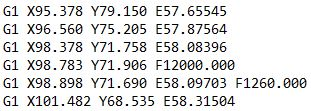
\includegraphics[width = 0.45\textwidth]{Bilder/gcode_erklaerung}
			\par\end{centering}
			\caption{Maschinencode Erklärung}
			\label{gcode_erklaerung}
			\end{figure}

			% Table generated by Excel2LaTeX from sheet 'Tabelle1'
			\begin{table}[htbp]
  		\centering
  		\caption{Befehle G Code}
	    \begin{tabular}{ll}
	    G1    & Kontrollierte Bewegung \\
	    X, Y  & Koordinaten in horizontaler und vertikaler Richtung \\
	    E     & Angabe der Menge des Filaments, dass in den Extruder geschoben werden muss \\
	    F     & Geschwindigkeit, mit der das Material in den Extruder geschoben wird (mm/min) \\
	    \end{tabular}%
	  	\label{tab:befehle gcode}%
			\end{table}%

		Je nachdem wie der Drucker aufgebaut ist, werden die Produkte genau oder nur grob angefertigt. Sehr genaue Teile kann man am besten in einem Drucker produzieren, der einen geschlossenen Druckraum \bzw eine beheizte Druckplatte hat.
		Besonders an dünnen Platten merkt man das. Wenn der Druckraum nach \bzw während des Druckvorgangs warm ist, kühlt das Werkstück an jeder Stelle fast gleich ab.
		Ist der Druckraum offen, kühlt das Werkstück in der Mitte schneller ab, kühles Material zieht sich zusammen, daher biegt sich das Material auf.

		Es kann vorkommen, dass ein Teil nur so gedruckt werden kann, wenn es nicht komplett auf der Druckplatte aufliegt zum Beispiel ein Steg, der „in der Luft“ liegt oder eine Bohrung im Werkstück, die horizontal gedruckt werden muss.
		In solchen Fällen, druckt der Drucker unter diesem Steg Stützmaterial. Basierend auf diesem Stützmaterial, wird dann die gewünschte Form gedruckt.
		Das Stützmaterial ist so gefertigt, dass man es leicht von dieser abbrechen kann, ohne dass Rückstände zurück bleiben.

		\subsubsection{Von der Idee zur Anfertigung}

		Die größte Hürde an der Realisierung einer Idee ist, eine CAD Zeichnung zu erstellen. In 3D CAD Programmen wie Creo, SolidWorks, etc. kann man ein Teil konstruieren und dann als STL (Standard Triangulation Language) File abspeichern.
		Dieses Format gibt dann nur mehr Informationen über die Oberfläche und Struktur an (siehe Abbildung \ref{stl_file_optionen}).
		Die Sehnenhöhe gibt an wie genau die Oberfläche gedruckt werden muss, die Winkelsteuerung gibt die Genauigkeit der Radien und Kanten des Teiles an.


			\begin{figure}[tbh]
			\begin{centering}
			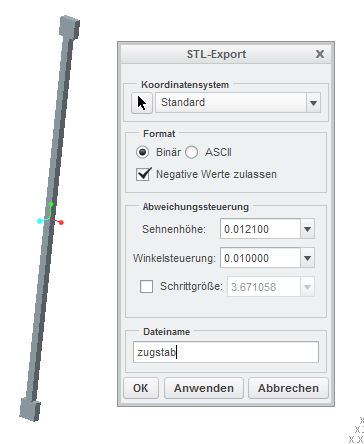
\includegraphics[width = 0.5\textwidth]{Bilder/stl_file_optionen}
			\par\end{centering}
	 		\caption{Einstellung für STL File}
			\label{stl_file_optionen}
			\end{figure}

		Mit diesem File kann man anschließend in Programmen wie Slic3r den gewünschten Maschinencode generieren lassen.
		In diesen Programmen gibt man die Lage des Werkstückes an \bzw in genaueren Einstellungen auch die Temperatur des Druckbettes, den Geschwindigkeiten und ähnliche Konfigurationen.

		Am häufigsten haben die Drucker eine USB Schnittstelle, \bzw verfügen über einen SD Karten Slot.
		Der Maschinencode wird auf diesen Speichermedien gespeichert und einfach auf den Drucker überspielt.

				\newpage


\section{Halterung für Cupcakes}

		\subsection{Technische Planung}

		Die Diplomarbeit hat sich speziell auf den Transport von Cupcakes spezialisiert, um diesen sicher transportieren zu können, ist es notwendig eine Halterung zu konzipieren.
		Zu beachten ist, dass die Halterung möglichst wenig wiegt \bzw leicht zu montieren ist.

		Der Akku wurde an der Unterseite des Hexacopters befestigt, daher war es nur mehr möglich die Halterung an der oberen Centerplate zu platzieren.
		Damit der Multicopter möglichst ausgewogen ist, muss sich das zu transportierende Objekt in der Mitte befinden.
		Die Idee war es daher, den Cupcake mit einer Halterung zu umranden, um ihn gegen Verrutsche zu sichern. Die Geometrie der Platte \bzw die Größe des Objektes hat die Befestigungsmöglichkeiten etwas eingeschränkt (siehe Abbildung \ref{platte_cupcake}).
		Die innere Reihe der Langlöcher würde sich optimal anbieten, um die Halterung befestigen zu können, die Cupcakeform kann so direkt von einer Haltevorrichtung gestützt werden.


			\begin{figure}[tbh]
			\begin{centering}
			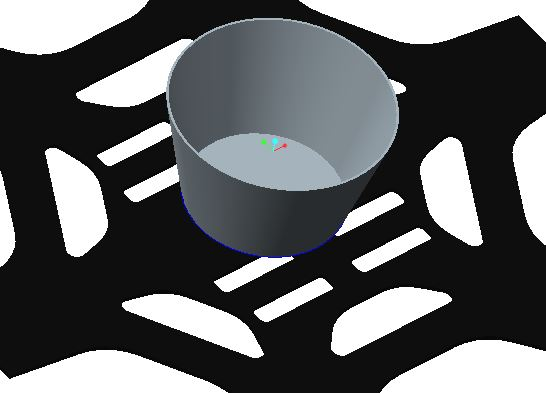
\includegraphics[width = 0.5\textwidth]{Bilder/platte_cupcake}
			\par\end{centering}
			\caption{Position Cupcake}
			\label{platte_cupcake}
			\end{figure}

	\subsection{Umsetzung}

	Wie schon in der technischen Planung erwähnt wurde, sollte der Cupcake von einer Haltevorrichtung umrandet werden.
	Die inneren Ausnehmungen der oberen Centerplate haben sich optimal angeboten, da diese direkt bis zur Form reichen.

	Es wurden Stützen konstruiert, die in den Ausnehmungen fixiert werden können und sich direkt an das Dessert anpassen.
	Die folgenden Abbildungen zeigen die konstruierten Halterungsstutzen und deren Befestigung.

			\begin{figure}[H]
			  \begin{centering}
			    \subfigure[Halterung Cupcake oben\label{halterung_cupcake_oben_grosz}]{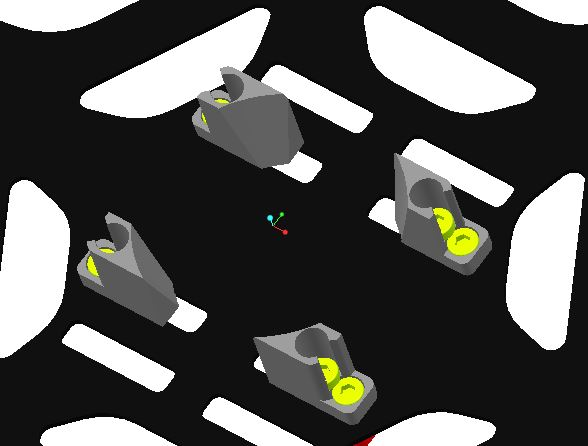
\includegraphics[width = 0.4\textwidth]{Bilder/halterung_cupcake_oben_grosz}}
			    \subfigure[Halterung Cupcake unten\label{halterung_cupcake_unten_grosz}]{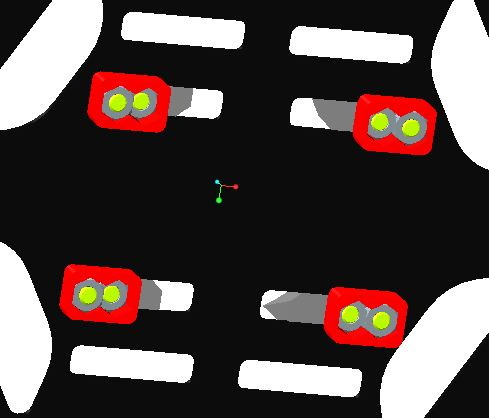
\includegraphics[width = 0.4\textwidth]{Bilder/halterung_cupcake_unten_grosz}}
			  \par\end{centering}
			  \caption{Halterung Cupcake}
			  \label{Halterung_Cupcake}
			\end{figure}

	Die Stützen (siehe Abbildung \ref{halterung_cupcake_oben_grosz}) wurden so entworfen, dass sie sich dem Radius \bzw der Höhe der Form des Cupcake anpassen.
	Die Höhe der Halterung wurde so gewählt, dass etwa die Hälfte der Cupcakeform frei liegt.
	Das soll vermeiden, dass man sich die Finger beim Entnehmen des Cupcakes an der Creme schmutzig macht.

	Die Halterung wird direkt an der Centerplate mit Durchgangsschrauben und Muttern festgeschraubt.
	Durch den Platzmangel mussten M4 Schrauben gewählt werden, da diese klein sind und trotzdem viel Beanspruchung aufnehmen können.
	Die Schlüsselweite einer M4 Mutter beträgt 7.0 mm, die Breite der Ausnehmung 6.5 mm, würde man die Schrauben direkt mit der Platte verschrauben, müsste man eine Beilagscheibe zwischenlegen, um eine größere Aufliegefläche für die Mutter zu erhalten.

	Es wurden spezielle Mutterhalter entworfen (siehe Abbildung \ref{halterung_cupcake_unten_grosz}), diese bezwecken zwei Funktionen:
	Einerseits muss man die Muttern während man die Halterung montiert nicht mehr festhalten und andererseits kann man die Schraubenverbindung viel fester anziehen, da man die Platte nicht mehr beschädigen kann.

	Der Platz für die Stutzen entlang der Langlöcher ist nur so kurz, dass sich die Köpfe der Schrauben und die Muttern schneiden würden.
	Um dieses Problem zu beheben, wurden Höhenunterschiede zwischen den Schrauben eingeplant.
	Das macht die Halterungsstutzen kompakter und verhindert Kollisionen.

	\subsection{Herausforderungen und Lösungen}

	Die größte Herausforderung beim Konstruieren war es, die Halterung an die Form des Cupcakes anzupassen.
	Die Halterungsstützen sollen an die Rundung \bzw den Durchmesserverlauf der Cupcakeform angepasst werden.
	Um die richtige Form der Stützen konstruieren zu können, wurde erst der Winkel der Cupcakeform mit der  folgenden Formel ermittelt:

			\begin{figure}[H]
			\begin{centering}
			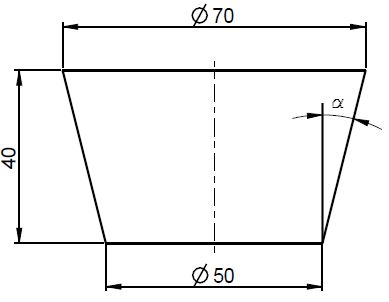
\includegraphics[width = 0.4\textwidth]{Bilder/berechnung_winkel}
			\par\end{centering}
			\caption{Berechnung des Winkels}
			\label{berechnung_winkel}
			\end{figure}

			\[
 				\tan \alpha = \frac{35mm-25mm}{40mm}  \qquad \alpha = \arctan \frac{35mm-25mm}{40mm} = \SI{14.04}{\degree}
 			\]

	Konstruiert wurde die Halterung mit einem Winkel von 15° um Ungenauigkeiten des Druckers besser kompensieren zu können.

	In der folgenden Abbildung kann man erkennen, dass manche Wände bei den Bohrungen zu dünn sind zu drucken, es entstehen dadurch Löcher.
	Dieses Problem könnte man nur lösen, wenn man die Schrauben weiter nach außen legen würde, jedoch ist das in diesem Fall nicht möglich, da die Ausnehmungen zu kurz sind.


			\begin{figure}[tbh]
			\begin{centering}
			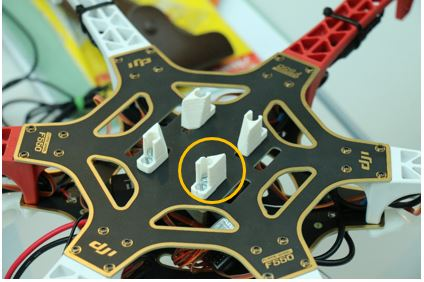
\includegraphics[width = 0.65\textwidth]{Bilder/halterung_cupcake_fertig_hinweis}
			\par\end{centering}
			\caption{Gedrucktes Halterungssystem}
			\label{halterung_cupcake_fertig_hinweis}
			\end{figure}

			\newpage

\section{Rotorschutz}

	\subsection{Technische Planung}

	In dem gewählten Bausatz des Hexacopters ist kein Rotorschutz vorhanden.
	Da der Hexacopter direkt zu den Gästen fliegen wird, ist es nicht umgänglich, den Kontakt mit den Propellern zu verhindern.
	Diese können durch die hohen Drehzahlen und die Kraft der Motoren erhebliche Verletzungen zuführen.
	Es gibt diverse Vorrichtungen für Multicopter zu kaufen, die nur die Rotorblätter schützen, jedoch keine, die auch das Eingreifen einer Hand verhindern.

	Der Rotor-, oder auch Propellerschutz genannt, soll wie ein Ring um die Rotorblätter liegen und auch auf der Ober,- und Unterseite Schutz vor Verletzungen bieten.
	Zu beachten ist jedoch auch, dass sechs Schutzvorrichtungen benötigt werden, daher sollten diese so leicht wie möglich sein, um das maximale Abfluggewicht nicht zu überschreiten.

	\subsection{Umsetzung}

	Die folgenden Abbildungen zeigen den konstruierten Propellerschutz, an dem Hexacopter montiert.

			\begin{figure}[tbh]
			\begin{centering}
			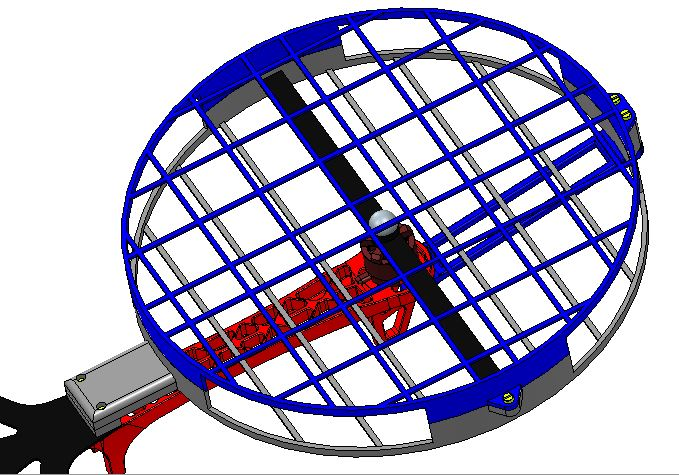
\includegraphics[width = 0.8\textwidth]{Bilder/propellerschutz_gesamt_oben}
			\par\end{centering}
			\caption{Propellerschutz oben}
			\label{propellerschutz_gesamt_oben}
			\end{figure}

			\begin{figure}[H]
			\begin{centering}
			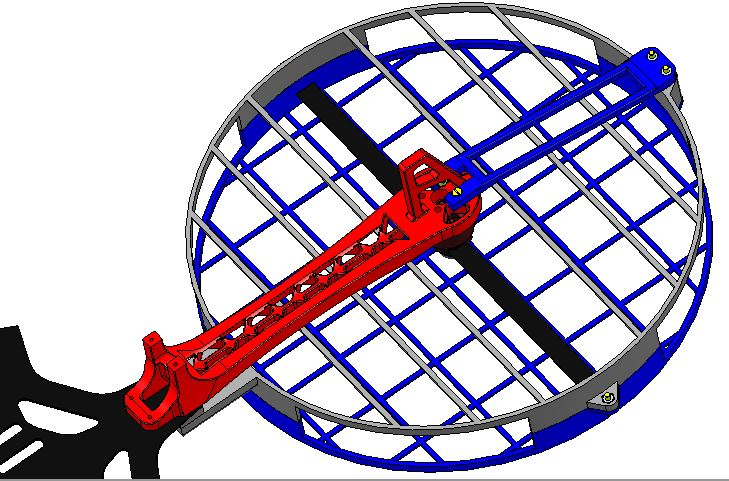
\includegraphics[width = 0.8\textwidth]{Bilder/propellerschutz_gesamt_unten}
			\par\end{centering}
			\caption{Propellerschutz unten}
			\label{propellerschutz_gesamt_unten}
			\end{figure}

	Wie geplant, umrandet der Ring das komplette Rotorblatt, im Falle eines Absturzes kann der Propeller nicht den Boden berühren und wird somit nicht beschädigt.
	Auf der Oberseite und Unterseite ist ein Gitter vorgesehen, welches Verletzungen an Personen verhindert.
	Das Gitter an der Oberseite ist etwas feiner gegliedert als an der Unterseite, da man den Cupcake von der oberen Centerplate entnehmen muss.
	An der Unterseite ist das Gitter nur gestreift konstruiert, da die Luftströmung nicht stark beeinflusst werden darf und die größere Verletzungsgefahr an der Oberseite besteht.

	Der komplette Rotorschutz wird einerseits mit zwei Schrauben am Hexacopter befestigt (siehe Abbildung \ref{propellerschutz_gesamt_oben}) und andererseits von einer Stütze (siehe Abbildung  \ref{propellerschutz_gesamt_unten},
	\textcolor{blue}{blauer Balken}) an der Unterseite gehalten. Die Stütze wird direkt an dem Motor angeschraubt, samt dem Arm des Hexacopters.
	Da die Schrauben der Centerplate und des Motors zu kurz sind, werden passende Zylinderkopfschrauben verwendet.
	Besonders bei dem Motor ist es wichtig, dass diese nicht zu lang sind, da sich der Motor nicht mehr bewegen könnte.

	Durch die Gewichtsbegrenzung \bzw der Form des Propellerschutzes, bot es sich an, diesen in einem 3D Drucker anzufertigen.
	Dazu wurde der Ring in zwei Hälften unterteilt, eine Ober,- und eine Unterseite.
	Der Ring hat einen ungefähren Innendurchmesser von 270 mm, das Druckbett eine maximale Abmessung von 270x210 mm.
	Beide Hälften mussten noch in weitere, für den Drucker passende Teile unterteilt werden.
	Die obere Hälfte wurde noch einmal in der Mitte geteilt, die Unterseite musste in vier Teile unterteilt werden (siehe folgende Abbildung \ref{propellerschutz_mitte_unterteilung}).

			\begin{figure}[tbh]
			\begin{centering}
			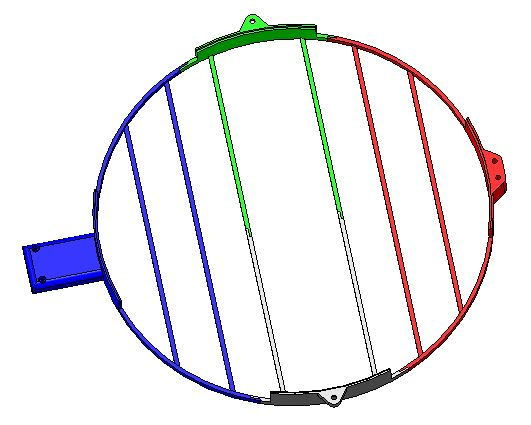
\includegraphics[width = 0.7\textwidth]{Bilder/propellerschutz_mitte_unterteilung}
			\par\end{centering}
			\caption{Propellerschutz Unterteilung}
			\label{propellerschutz_mitte_unterteilung}
			\end{figure}

			\begin{figure}[H]
			\begin{centering}
			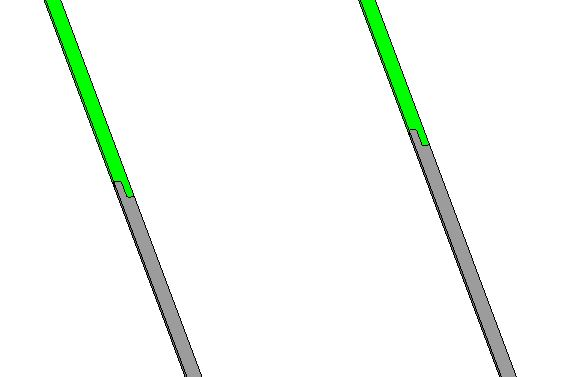
\includegraphics[width = 0.45\textwidth]{Bilder/propellerschutz_klebestellen}
			\par\end{centering}
			\caption{Propellerschutz Klebestellen}
			\label{propellerschutz_klebestellen}
			\end{figure}

	Die einzelnen Hälften  werden mit Sekundenkleber zusammengefügt, die Klebestellen wurden daher mit Nuten versehen,
	um eine größere Klebefläche zu gewährleisten (siehe Abbildung \ref{propellerschutz_klebestellen}).
	Die geklebten Hälften werden dann mit Durchgangsschrauben und Sechskantmutter miteinander verschraubt (siehe Abbildung  \ref{propellerschutz_mitte_unterteilung}),
	der kleine Absatz an der unteren Hälfte wird extra angefertigt da der Drucker kein Stützmaterial drucken müsste.

	\subsection{Herausforderungen und Lösungen}

	Eines der größten Probleme war es, den Rotorschutz so zu konstruieren, dass er stabil, aber auch sehr leicht ist.
	Im Falle eines Absturzes, würden hohe Kräfte auf den Propellerschutz wirken, daher muss dieser sehr robust gefertigt sein.
	Der Vorteil von ABS \bzw 3D Druckteilen ist, dass diese sehr elastisch sind, nicht wie Styropor zum Beispiel, es ist daher nicht notwendig den Ring dickwandig zu konstruieren.
 	Durch diesen Vorteil kann man einiges an Gewicht einsparen, das Problem besteht aber trotzdem noch darin, dass der Ring enorme Dimensionen hat.
	Eine komplette Zusammenstellung (Ring, Stütze und Schrauben) hat ein Gewicht von etwa 90 g.
	Auf sechs Propeller aufgerechnet mehr als ein halbes Kilogramm, der Hexacopter kann das zwar noch tragen, jedoch schränkt das die hardwaremäßige Erweiterung stark ein.

	Eine weitere Herausforderung war es, den Ring anzufertigen. Wie schon in dem oberen Punkt erklärt wurde, musste der Ring in sieben Teile unterteilt werden.
	Die Herausforderung lag darin, die Stücke so zu gliedern, damit sie im 3D Drucker fertigbar sind und nicht zu viel Druckzeit auf sich nehmen.
	Die Druckzeit wurde zwar schon optimiert durch die Gliederung, jedoch braucht es trotzdem noch etwa 14 Stunden alle Teile für einen Rotorschutz zu drucken.

	\subsection{Implementierung}

Die einzelnen Teile wurden wie schon erwähnt, miteinander verklebt. Bevor diese zusammengefügt wurden, musste sichergestellt werden, dass die Nuten exakt ineinander passen.
Würde dies nicht gewährleistet sein, würden die obere und untere Hälfte des Propellerschutzes nicht mehr zusammenpassen.
Die Toleranzen des Druckers, besonders bei solchen Stellen sind so groß, dass man meistens mit Feilen die Nuten nachbessern muss.
Besonders beim Verkleben der Teile ist viel Geduld nötig, da auch der Sekundenkleber nicht sofort komplett trocken ist,
es war ebenso wichtig, den richtigen Untergrund zu wählen, eine Holzplatte eignete sich am besten, da keine Rückstände blieben.

Die beiden Hälften wurden dann miteinander verschraubt, samt der Stütze.
Der gesamte Rotorschutz konnte dann mittels den vorgesehenen Schrauben an der Centerplate und dem Arm des Hexacopters befestigt werden.

			\newpage

\section{Halterung Ultraschallsensor}

	\subsection{Technische Planung}

	Die Höhe des Hexacopters wird mittels eines Ultraschallsensors gesteuert, dieser misst den Abstand von dem Boden aus.
	Damit der Sensor genaue Werte messen kann, muss er fest auf dem Multicopter befestigt werden.
	Um das gewährleisten zu können, musste eine Halterung entworfen werden, die den Ultraschallsensor optimal mit dem Hexacopter verbindet.
	Die Anforderungen an die Halterung begrenzen sich auf ein geringes Gewicht \bzw eine einfache Montagemöglichkeit.
	Der Sensor hat auf jeder Ecke eine kleine Bohrung von 1.5 mm vorgesehen, das erschwert die Befestigungsmöglichkeit des Sensors an der Halterung, da es keine gängigen Schrauben in dieser Größe gibt.

	\subsection{Umsetzung}

	Die folgende Abbildung (Abbildung \ref{halterung_ultraschall}) zeigt die CAD Konstruktion und die gefertigte (Abbildung \ref{halterung_ultraschall_fertig}) Ultraschallsensorhalterung.

			\begin{figure}[H]
				\begin{centering}
					\subfigure[CAD Konstruktion Ultraschallsensorhalterung\label{halterung_ultraschall}]{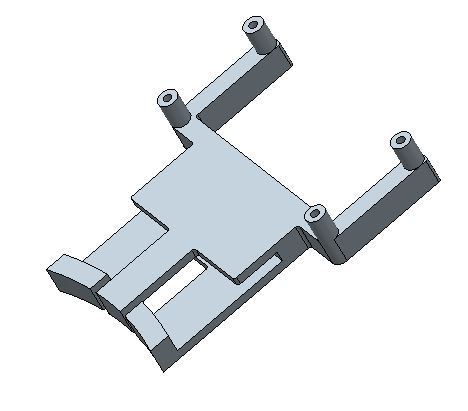
\includegraphics[width = 0.4\textwidth]{Bilder/halterung_ultraschall}}
					\subfigure[Gefertigte Ultraschallsensorhalterung\label{halterung_ultraschall_fertig}]{\includegraphics[width = 0.4\textwidth]{Bilder/halterung_ultraschall_fertig}}
				\par\end{centering}
				\caption{Ultraschallsensorhalterung}
				\label{Halterung_Ultraschallsensor}
			\end{figure}

	Das Gewicht spielte, analog zu den anderen Konstruktionen, eine wichtige Rolle.
	Materialien wie Stahl oder Aluminium wären selbst bei diesem kleinen Teil (51x46x10 mm) zu schwer geworden.
	Um das zu verhindern wurde diese Haltevorrichtung, wie auch der Propellerschutz, in einem 3D Drucker angefertigt.
	Das Teil wiegt durch die Fertigungsmethode etwa 5.5 g, das entspricht etwa dem Gewicht einer 20 Cent Münze.

	Die Halterung wird an der unteren Centerplate befestigt, da wie schon erwähnt, der Sensor von dem Boden aus misst.
	Die Befestigungsmethode ist selbst entwickelt worden, dabei handelt es sich um ein spezielles Klammersystem, welches an einer Strebe der Platte montiert werden kann (siehe Abbildung \ref{halterung_ultraschall_fertig}).
	Die Klammer besteht aus drei Stegen, auf denen jeweils ein Anschlag vorgesehen wurde.
	Die Form der Anschläge ist  exakt an die Centerplate angepasst, damit sich die Halterung so geringfügig wie möglich bewegen lässt.

	Die ideale Stärke der Stege wurde durch Versuche ermittelt, es wurde dabei das Klammersystem mit unterschiedlichen Dicken gefertigt und an dem Hexacopter getestet.
	Die optimale Stärke war deshalb wichtig, da das System nicht funktionieren würde, wenn diese falsch dimensioniert werden würde.
	Die Elastizität des Materials \bzw die gewählte Dicke der Stege ermöglicht es, diese soweit auseinanderziehen zu lassen, dass die Anschläge einfach über die Platte geschoben werden können.
	Aufgrund dieser Eigenschaften verformen sich diese auch wieder komplett zurück und fixieren somit die Halterung.

	Damit der Sensor nicht nach unten kippen kann, wurde eine Nut in die Haltevorrichtung vorgesehen.
	Droht die Halterung nach unten zu kippen, verkeilt sich diese mit der Centerplate und kann nicht mehr weitersinken.
	Die Nut ist so groß dimensioniert worden, dass sie leicht auf die Platte geschoben werden aber sich nur minimal bewegen lässt.

	Der zweite Teil der Halterung wurde so konstruiert, dass die vier Ecken der Sensorplatine gleichmäßig aufliegen können.
	Auf dem Ultraschallsensor selbst befinden sich jedoch vier Anschlussstifte, die es nicht ermöglichen, die Platine direkt auf der „Gabel“ zu befestigen.
	Um Kabel trotzdem problemlos anschließen zu können, wurde der Sensor mittels vier Stutzen 5 mm höher gelegt.

	Geplant wurde, dass der Sensor an den Stutzen mit vier Blechschrauben befestigt wird, die Durchmesser der Bohrungen sind aber so klein, dass keine gängigen Schraubendurchmesser verwendet werden können.
	Die geeigneten Schrauben werden nur in ausgewählten Geschäften verkauft, um einen viel höheren Preis \bzw längeren Lieferzeiten, als bei normalen Schrauben.
	Um den Sensor trotzdem befestigen zu können, wurden Kupferdrähte zur Fixierung verwendet.
	Da nur das Gewicht des Ultraschallsensors an den Drähten zieht, geben diese selbst bei heftigen Flugmanövern nur minimal nach.

	\subsection{Herausforderungen und Lösungen}

	Das Klammersystem hat die meiste Zeit auf sich genommen.
	Die erste Version der Halterung hat gezeigt, dass die angenommenen Dimensionen nicht umgesetzt werden konnten.
	Das Problem lag darin, dass die Halterung nicht hochkant, sondern vertikal gedruckt werden musste.
	Damit die Haltevorrichtung gedruckt werden kann, hat der Drucker Stützmaterial in die Nut gedruckt.
	Dieses Stützmaterial kann jedoch nicht restlos entfernt werden, daher musste die Höhe des Spaltes vergrößert werden.
	Es brauchte drei verschiedene Versionen der Ultraschallsensorhalterung, bis alle Parameter ideal gepasst haben, das kostete natürlich Zeit, da jedes Mal ein neues Teil gedruckt werden musste.

	\subsection{Berechnungen}

	Die Halterung des Ultraschallsensor wurde so dimensioniert, dass der Ultraschallsensor, \bzw im Falle eines Absturzes auch noch die auftretenden Kräfte getragen werden können,
	es ist trotzdem wichtig zu wissen, wie viel die Halterung maximal tragen kann.
	Sollte sich herausstellen, dass das Werkstück nicht richtig konstruiert wurde, müssen Maßnahmen getroffen werden um die Belastbarkeit zu steigern.

	Man kann diese Belastungen händisch rechnen, jedoch ist das in diesem Fall sehr aufwändig, da die Lagerung sehr komplex zu rechnen wäre.
	Es ist einfacher die Beanspruchungen in Programmen wie Creo simulieren und auswerten zu lassen.
	Die Ergebnisse der Simulation sind so genau, dass man heutzutage in der Industrie nur mehr sehr selten solche Arten von Analysen händisch vornimmt.

	Die maximalen Belastbarkeiten sind für jeden Kunststoff anders, jede Firma verwendet andere Stoffe um bessere Leistungen erzielen zu können, je nach dem Anwendungsgebiet.
	Wollte man die Berechnungen auf die Kommastelle genau vornehmen, müsste man einen Zug,- oder Biegeversuch für den jeweiligen Werkstoff machen,
	um die tatsächlichen Daten zu ermitteln.

	In diesen Versuchen wird meist ein Stab mit einer vordefinierten Fläche und Länge hergestellt und dann in eine Zugprüfmaschine eingespannt.
	Die Zugprüfmaschine zieht den Stab langsam auseinander bis dieser reißt, diese bestimmte Kraft und die Fläche des Stabes ergeben die maximale Streckspannung.
	Diesen Versuch kann man analog dazu für die Biegung und Torsion machen, man erhält dadurch die maximale Bruch,- \bzw Torsionsspannung.

	Da sich die Werte der einzelnen Hersteller nur minimal voneinander unterscheiden,
	wurden in diesem Fall die Daten aus einer Tabelle eines anderen Kunstoffherstellers genommen (siehe Abbildung \ref{werte_abs}).

			\begin{figure}[H]
			\begin{centering}
			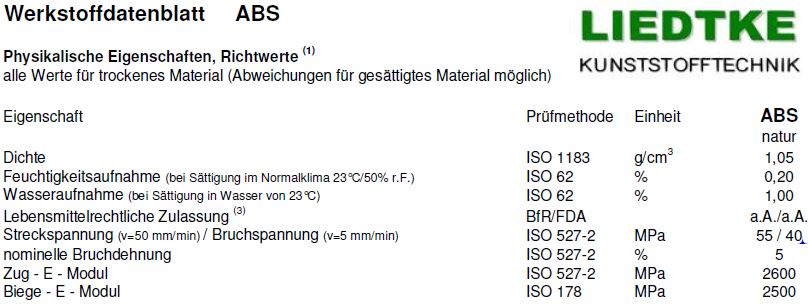
\includegraphics[width = 1\textwidth]{Bilder/werte_abs}
			\par\end{centering}
			\caption[Werte ABS]{Werte für ABS\cite{werte_abs}}
			\label{werte_abs}
			\end{figure}

	Wichtig sind die Angaben: Dichte, Streck,- und Bruchspannung, nominelle Bruchdehnung und Elastizitätsmodul für Zug/Biegung (E-Modul) des Materials.
	Diese Werte definieren die Eigenschaften des Materials, daher sind sie essenziell für die Berechnungen in Creo.

	Creo bietet mit seinen Funktionen exakte Analysen an, die die maximalen Belastbarkeiten so genau berechnen wie sie tatsächlich auftreten.
	In diesem Fall wurde die prinzipielle Situation simuliert, die Werte stimmen nicht exakt mit den realen Kräften überein, jedoch reichen diese um zu sehen, was passiert.

	In Creo steht eine große Auswahl an Einspannmöglichkeiten bis zu Belastungen für ein Werkstück zu Verfügung (siehe folgende Abbildung).

			\begin{figure}[H]
			\begin{centering}
			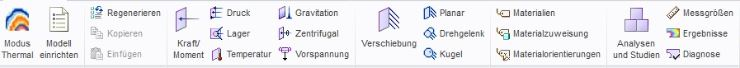
\includegraphics[width = 1\textwidth]{Bilder/auswahl_creo}
			\par\end{centering}
			\caption{Auswahlmenü Simulation}
			\label{auswahl_creo}
			\end{figure}

	Unter dem Menü „Verschiebung“ wird die gewünschte Lagerung definiert, man kann eine Fläche, Punkt oder Kante auswählen,
	je nachdem wie das Prüfwerkstück gelagert werden soll und in welche Richtung dieses verschiebbar ist.
	In dem Menü „Kraft/Moment“ gibt man dann an welche Belastung, in welcher Fläche/Punkt/Kante auf das Werkstück wirkt. Der Auswahlpunkt „Analysen und Studien“ startet die Simulation.

	Der Sensor wird so montiert, dass er die Halterung nach unten zieht, die Folge ist, dass sich die Halterung, grob angenommen,
	sich mit zwei Kanten an der Platte verkeilt (siehe Abbildung \ref{lager_darstellung_1} und \ref{lager_darstellung_2}).
	Die Lagerung wird daher so definiert, dass diese zwei Kanten als Festlager angenommen werden (in keine Richtung verschiebbar).

			\begin{figure}[H]
				\begin{centering}
					\subfigure[Lagerung 1. Stelle\label{lager_darstellung_1}]{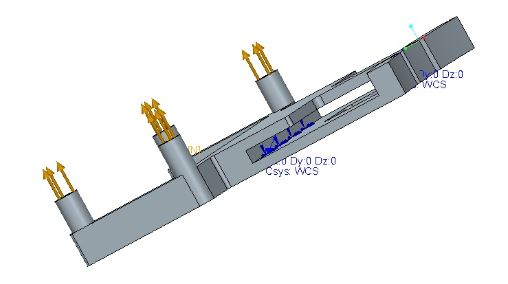
\includegraphics[width = 0.4\textwidth]{Bilder/lager_darstellung_1}}
					\subfigure[Lagerung 2. Stelle\label{lager_darstellung_2}]{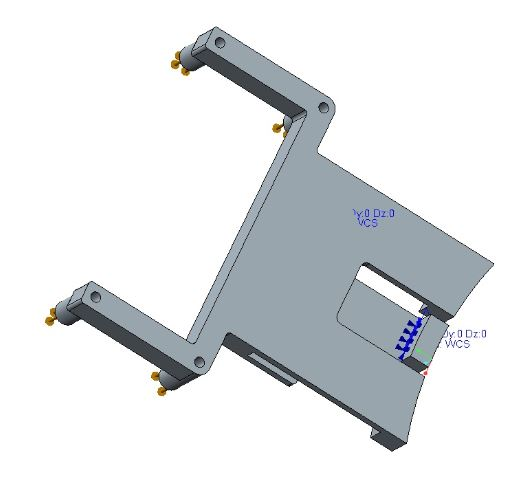
\includegraphics[width = 0.4\textwidth]{Bilder/lager_darstellung_2}}
				\par\end{centering}
				\caption{Lagerung der Halterung in Simulation}
				\label{Lagerung_Halterung}
			\end{figure}

	Der Ultraschallsensor wird durch eine Kraft ersetzt, diese kann man variieren, je nachdem um wieviel die Halterung belastet werden soll.
	Nachdem alle Parameter definiert wurden, konnte die Simulation gestartet werden.

	Es wurden zwei Simulationen durchgeführt, in der ersten wurde nur der Ultraschallsensor (8.5 g) als Belastung angenommen und im zweiten Fall  wurde die Halterung mit einer Last von 2 kg beansprucht.

	Die Abbildung \ref{max_spannung_f0_1_r0_5} zeigt das Ergebnis der ersten Simulation mit einer Kraft von 0.1 N (0,01 g).

			\begin{figure}[H]
			\begin{centering}
			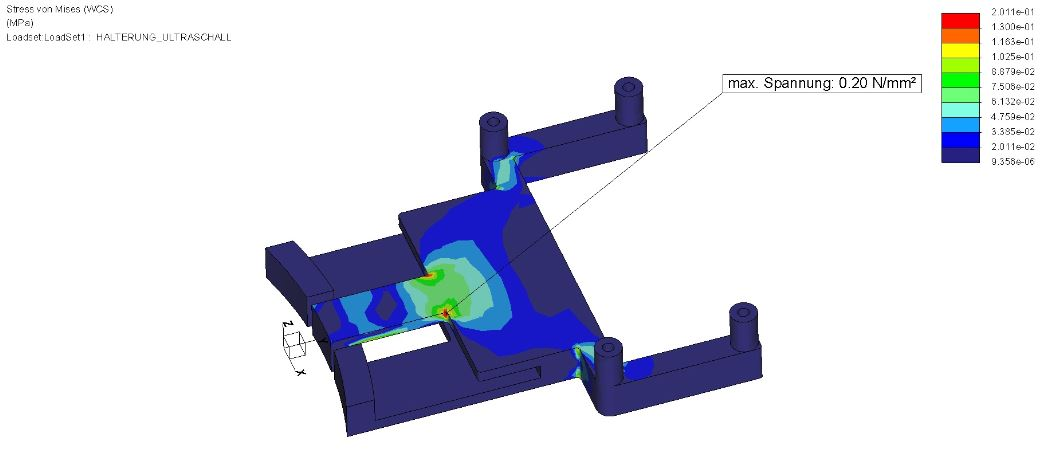
\includegraphics[width = 1\textwidth]{Bilder/max_spannung_f0_1_r0_5}
			\par\end{centering}
			\caption{max. Spannung bei 0.1 N}
			\label{max_spannung_f0_1_r0_5}
			\end{figure}

	Die maximale Spannung beträgt in diesem Fall etwa $0.20 N/mm^{2}$ an der oberen Lasche.
	Es ist zu sehen, dass diese Belastung die Halterung kaum beeinflusst, das bedeutet die angenommen Dimensionen reichen aus um den Sensor zu halten.

	Die Abbildungen \ref{max_spannung_f20_r0_5} und \ref{max_spannung_f20_r0_5_oben}  zeigen die Simulationsergebnisse mit einer Beanspruchung von 20 N (2 kg).

			\begin{figure}[H]
			\begin{centering}
			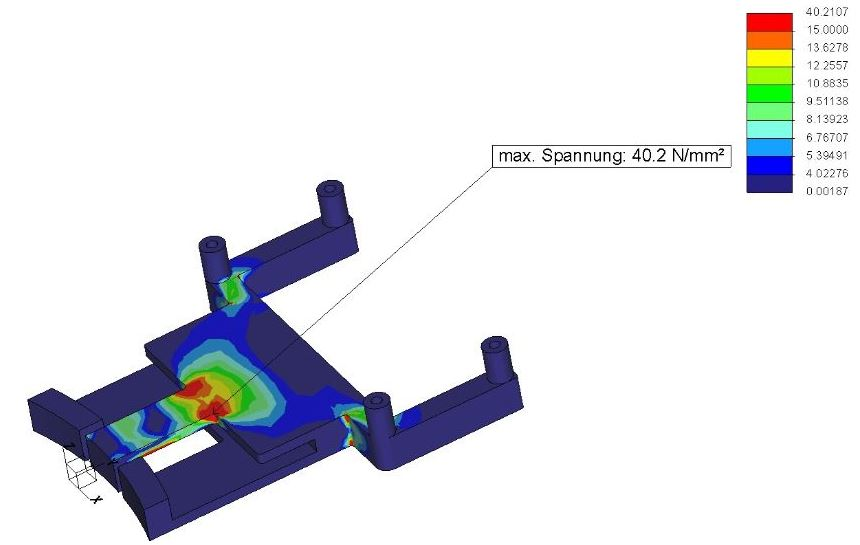
\includegraphics[width = 1\textwidth]{Bilder/max_spannung_f20_r0_5}
			\par\end{centering}
			\caption{max. Spannung bei 20 N}
			\label{max_spannung_f20_r0_5}
			\end{figure}

			\begin{figure}[H]
			\begin{centering}
			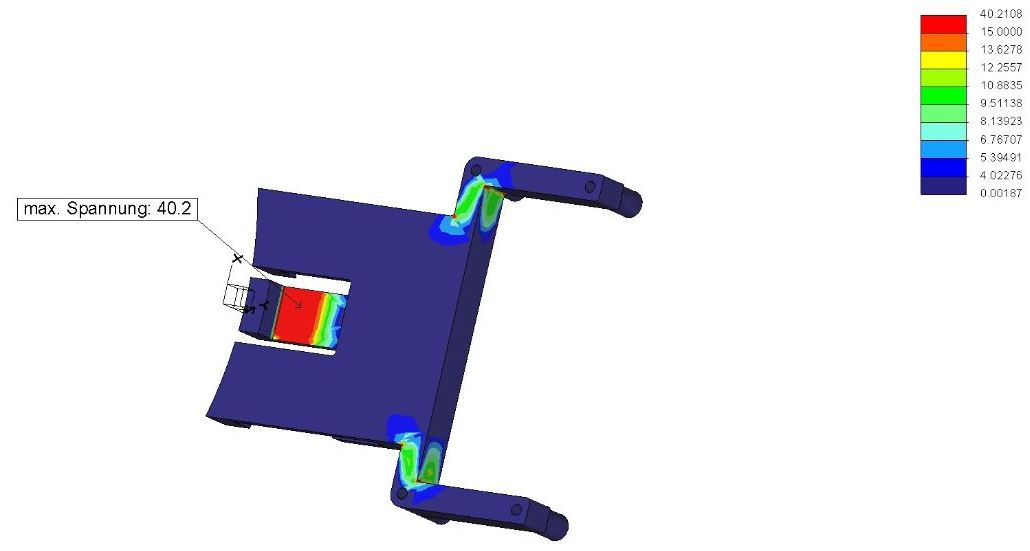
\includegraphics[width = 1\textwidth]{Bilder/max_spannung_f20_r0_5_oben}
			\par\end{centering}
			\caption{max. Spannung bei 20 N}
			\label{max_spannung_f20_r0_5_oben}
			\end{figure}

				%\begin{figure}[H]
				%	\begin{centering}
				%		\subfigure[max. Spannung bei 20 N oben\label{max_spannung_f20_r0_5}]{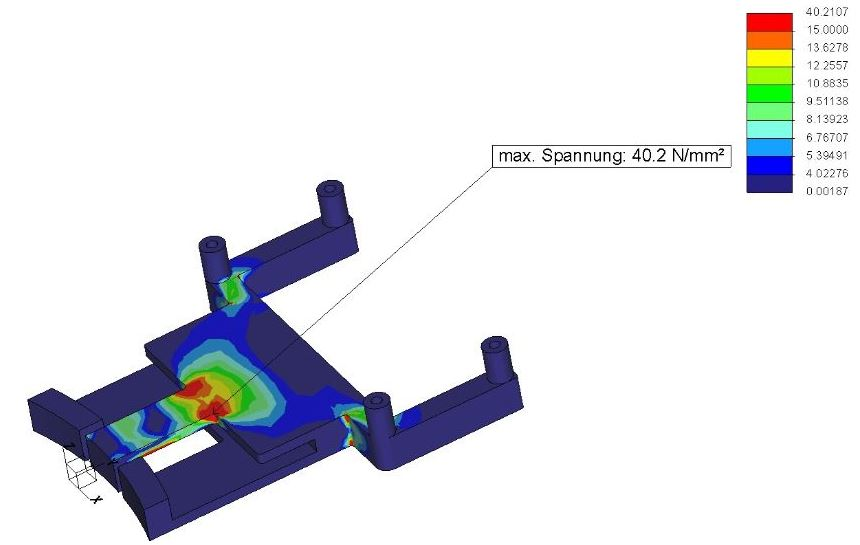
\includegraphics[width = 0.4\textwidth]{Bilder/max_spannung_f20_r0_5}}
				%		\subfigure[max. Spannung bei 20 N unten\label{max_spannung_f20_r0_5_oben}]{\includegraphics[width = 0.4\textwidth]{Bilder/max_spannung_f20_r0_5_oben}}
				%	\par\end{centering}
				%	\caption{max. Spannung bei 20 N}
				%	\label{max_spannung_f20_r0_5}
				%\end{figure}

	Die maximale Spannung beträgt etwa $40.2 N/mm^{2}$, vergleicht man dies mit dem Ausschnitt aus dem Datenblatt (siehe Abbildung \ref{werte_abs}) sieht man,
	dass die maximale Biegespannung an beiden Stellen überschritten wurde. In der Realität würde das bedeuten, dass die Lasche bei dieser Belastung sehr stark verformt oder gar gebrochen wäre.
	Solche starken Beanspruchungen treten in diesem Fall niemals auf, da  bei einem Absturz die Halterung geschützt wäre.

	Um auch im Notfall hohe Belastungen kompensieren zu können, wurden in den Kanten der Laschen Rundungen vorgesehen. Den Zweck dieser Rundungen zeigen die folgenden Abbildungen.

			\begin{figure}[H]
			\begin{centering}
			\includegraphics[width = 1\textwidth]{Bilder/max_spannung_f20_r0_5}
			\par\end{centering}
			\caption{max. Spannung bei 20 N, Radius 0.5 mm}
			\label{max_spannung_f20_r0_5}
			\end{figure}

			\begin{figure}[H]
			\begin{centering}
			\includegraphics[width = 1\textwidth]{Bilder/max_spannung_f20_r1}
			\par\end{centering}
			\caption{max. Spannung bei 20 N, Radius 1 mm}
			\label{max_spannung_f20_r1}
			\end{figure}

			%\begin{figure}[H]
			%	\begin{centering}
			%		\subfigure[max. Spannung bei 20 N, Radius 0.5 mm\label{max_spannung_f20_r0_5}]{\includegraphics[width = 0.4\textwidth]{Bilder/max_spannung_f20_r0_5}}
			%		\subfigure[max. Spannung bei 20 N, Radius 1.0 mm\label{max_spannung_f20_r1}]{\includegraphics[width = 0.4\textwidth]{Bilder/max_spannung_f20_r1}}
			%	\par\end{centering}
			%	\caption{max. Spannung bei 20 N, unterschiedliche Radien}
			%	\label{max_spannung_f20_r0_5}
			%\end{figure}

	Abbildung \ref{max_spannung_f20_r0_5} zeigt die Beanspruchung von 2 kg und einem Radius von 0.5 mm.
	Das Ergebnis zeigt, wie schon erwähnt, dass die maximale Biegespannung überschritten wurde.
	Abbildung \ref{max_spannung_f20_r1}, zeigt das Ergebnis mit der gleichen Kraft, aber einem Radius von 1 mm, also doppelt so groß wie in der ersten Simulation.
	Man kann sehr gut erkennen, dass die Spannung von $40.2 N/mm^{2}$ auf $30.3 N/mm^{2}$ gesunken ist, also um fast das eineinhalb-fache.

	Dieses Vorkommen wird in der Mechanik als \textbf{Kerbwirkung} bezeichnet:

			\begin{figure}[H]
				\begin{centering}
					\subfigure[Spannungsverteilung ohne Kerbe\label{spannungsverteilung_ohne_kerbe}]{\includegraphics[width = 0.8\textwidth]{Bilder/spannungsverteilung_ohne_kerbe}}
					\subfigure[Spannungsverteilung mit Kerbe\label{spannungsverteilung_mit_kerbe}]{\includegraphics[width = 0.6\textwidth]{Bilder/spannungsverteilung_mit_kerbe}}
				\par\end{centering}
				\caption[Spannungsverteilung bei Zug und Biegung]{Spannungsverteilung bei Zug und Biegung\cite{spannungsverteilung}}
				\label{spannungsverteilung_ohne_kerbe}
			\end{figure}

	Abbildung \ref{spannungsverteilung_ohne_kerbe} zeigt die Spannungsverteilung in einem Zug,- \bzw Biegestab ohne Querschnittsbeeinflussungen.
	Im Vergleich dazu wird in der Abbildung \ref{spannungsverteilung_mit_kerbe}, die Spannungsverteilung mit dem Einfluss einer Kerbe dargestellt.
	Für weitere Erklärungen wird der erste Stab „A“ und der zweite „B“ genannt.

	Beansprucht man „A“ mit einer Kraft oder einem Moment, verteilt sich die Spannung gleichmäßig über das Werkstück.
	Wird „B“, auf Zug oder Biegung beansprucht, kann man erkennen, dass sich die Spannung nur unter dem Kerbengrund verteilt.
	Die Spannung „A“ wird in der Regel mit $\sigma_{n}$ bezeichnet und die maximale Spannung in „B“ mit $\sigma_{max}$.
	Bildet man die Division zwischen $\sigma_{n}$ und $\sigma_{max}$, erhält man die Formzahl $\alpha_{k}$.
	$\alpha_{k}$ kann niemals kleiner als 1 werden, das würde bedeuten, dass die Kerbe als Stärkung des Querschnitts gelten würde.

	Die Form der Kerbe ist maßgebend, da diese die Spitzenwerte der Spannung beeinflussen, wie in Abbildung \ref{kerbform} ersichtlich ist.

			\begin{figure}[H]
			\begin{centering}
			\includegraphics[width = 0.4\textwidth]{Bilder/kerbform}
			\par\end{centering}
			\caption[Spannungsverteilung bei verschiedenen Kerbformen]{Spannungsverteilung bei verschiedenen Kerbformen\cite{kerbformen}}
			\label{kerbform}
			\end{figure}

	Je scharfkantiger die Form ist, desto größer sind die maximalen Spannungen an der Kerbe, hingegen, je runder und größerer die Kerbe ist, desto besser werden die auftretenden Spannungen verteilt.

	In der Halterung sollen die Rundungen kein Schwächen des Querschnittes bezwecken, in diesem Fall haben diese eine andere Wirkung.
	Berechnet man sich die Fläche der Lasche mit einer scharfen Kante und einer runden,
	sieht man dass der Radius die Oberfläche \bzw das Volumen vergrößert (siehe folgende Abbildungen), daher ist auch mehr Widerstand vorhanden.

			\begin{figure}[H]
				\begin{centering}
					\subfigure[Fläche mit Radius\label{klammer_mit_radius}]{\includegraphics[width = 0.4\textwidth]{Bilder/klammer_mit_radius}}
					\subfigure[Fläche ohne Radius\label{klammer_ohne_radius}]{\includegraphics[width = 0.4\textwidth]{Bilder/klammer_ohne_radius}}
				\caption{Flächeneinfluss durch Radius}
				\par\end{centering}
				\label{klammer_radius}
			\end{figure}

	Ist ein Radius vorhanden, beträgt das Volumen etwas mehr als $948.3 mm^{3}$, dieses Volumen verringert sich auf $947.6 mm^{3}$, wenn die Kante keinen Radius hat. Die Differnz ist nicht sehr hoch, wirkt sich auf die Spannung trotzdem enorm aus.

			\newpage

\section{Halterung PIXY CMU cam5}

	\subsection{Technische Planung}

	Der Hexacopter soll dem Gast sein gewünschtes Dessert bringen, der Weg zu dem Gast wird über Farbcodes am Boden vorgegeben.
	Um dem Farbcode folgen zu können, wird eine PIXY CMU cam5 verwendet (genaueres siehe Kapitel Sensoren).

	Die Halterung soll so konstruiert werden, dass die Kamera während des Fluges nicht wackelt, das verhindert ungenaue \bzw falsche Messwerte.
	Besonders zu beachten ist, dass die PIXY Cam immer in die Flugrichtung ausgerichtet sein muss.
	Der Flightcontroller gibt dem Hexacopter eine fixe Orientierung vor, würde die Kamera nicht in diese Richtung messen, könnte es zu Fehlmessung kommen und den Multicopter falsch navigieren.

	\subsection{Umsetzung}

	In den folgenden Abbildungen wird einerseits die konstruierte Halterung Abbildung \ref{halterung_pixy_creo})
	und andererseits die Gefertigte  mit der PIXY CMU cam5 (Abbildung \ref{halterung_pixy}).

			\begin{figure}[thb]
				\begin{centering}
					\subfigure[CAD Konstruktion PIXY Cam Halterung\label{halterung_pixy_creo}]{\includegraphics[width = 0.3\textwidth]{Bilder/halterung_pixy_creo}}
					\subfigure[Gefertigte PIXY Cam Halterung\label{halterung_pixy}]{\includegraphics[width = 0.4\textwidth]{Bilder/halterung_pixy}}
				\par\end{centering}
				\caption{Halterung PIXY Cam}
				\label{Halterung_PIXY}
			\end{figure}

	Aus Gewichtsgründen wurde die Halterung in einem 3D Drucker angefertigt.
	Diese wiegt etwa 5.2 g, ist also etwas leichter als die Ultraschallsensorhalterung.
	Um den Hexacopter, selbst bei so geringen Massen besser ausgleichen zu können, wurden beide Befestigungsmöglichkeiten gegenüber voneinander platziert.
	Da die PIXY Cam Halterung auf der unteren Centerplate platziert wird, konnte wieder das eigens entwickelte Klammersystem verwendet werden.
	Das garantiert auch in diesem Fall eine gute Passgenauigkeit, um den Sensor optimal zu fixieren.

	Die Kamera hat an der unteren Leiste der Platine zwei Bohrungen vorgesehen, diese wurden genutzt um den Sensor mit der Halterung zu verbinden.
	Es bot sich nicht viel Platz auf der Platine an, um den Sensor fest genug zu fixieren, jedoch reichte der untere Streifen ausreichend aus.

	Wie schon in der technischen Planung erwähnt wurde, spielt die exakte Position der PIXY Cam eine wichtige Rolle.
	Die Vorgangsweise zur Ermittlung der Ausrichtung wird mit der folgenden Abbildung erklärt.

			\begin{figure}[tbh]
			\begin{centering}
			\includegraphics[width = 0.8\textwidth]{Bilder/winkel_pixy}
			\par\end{centering}
			\caption{Messung Winkel}
			\label{winkel_pixy}
			\end{figure}

	Der Flightcontroller wurde so eingebaut, dass ein Arm des Hexacopters zur Kontrolle in die Flugrichtung steht.
	Die \textcolor{red}{Halterung} wurde genau in der Mitte der Strebe platziert, daher konnte eine Konstruktionslinie vom Mittelpunkt der Platte aus, gesetzt werden.
	Der Winkel konnte gemessen werden, indem die zweite Konstruktionslinie entlang der Mitte des Arm gesetzt wurde.
	Die Schräge ist deshalb notwendig, da der Platz auf der Platine des Sensors so begrenzt ist, dass nur die Fläche der unteren Leiste aufliegen kann.

	\subsection{Herausforderungen und Lösungen}

	Der begrenzte Platz zum Montieren der PIXY Cam an der Halterung war die größte Herausforderung.
	Das  Problem war, dass sich auf der Platine eine Kabelbuchse befindet, diese ist genau auf der Ecke des Streifens vorgesehen (siehe Abbildung \ref{PIXY_Cam_Hinterseite}, orange markierter Bereich).

			\begin{figure}[H]
			\begin{centering}
			\includegraphics[width = 0.5\textwidth]{Bilder/PIXY_Cam_Hinterseite}
			\par\end{centering}
			\caption[PIXY Cam Anschlussbuchse]{PIXY Cam Anschlussbuchse\cite{PIXY_Cmu_cam5}}
			\label{PIXY_Cam_Hinterseite}
			\end{figure}

	In den Konstruktionen wurde dieses Problem nicht behandelt, erst bei dem ersten Test hat sich gezeigt, dass die Halterung nicht komplett passt.
	Um nicht noch eine neue Version drucken und Zeit verlieren zu müssen, wurde die Kante an der linken Bohrung (siehe Abbildung \ref{halterung_pixy_creo}) passgenau mit einer Feile abgerundet.

			\newpage

\section{Führung für Testflüge}

	\subsection{Technische Planung}

	Im Laufe des Projektes hat es sich bestätigt, dass es manchmal passieren kann, dass die Funkverbindung zwischen der Fernbedienung und dem Flugobjekt abbrechen kann.
	Ist jedoch keine Sicherung in der Firmware des Copters vorgesehen, fliegt dieser unkontrollierbar und stürzt ab.

	In diesem Projekt ist das Problem aufgetreten während eines Testfluges zur Testung der Höhenbestimmung durch den Ultraschallsensor.
	Damit dies nicht mehr vorkam, müsste eine Hardwaremäßige Vorrichtung entwickelt werden, die im Falle eines unvorhergesehenen Funkabbruches den Hexacopter sicher auf den Boden sinken lässt.

	\subsection{Umsetzung}

	Die folgende Abbildung zeigt die konstruierte (Abbildung \ref{gleitbuchse_creo}) und die gefertigte Gleitbuchse (Abbildung \ref{gleitbuchse_gefertigt}).

			\begin{figure}[tbh]
				\begin{centering}
					\subfigure[CAD Konstruktion Gleitbuchse\label{gleitbuchse_creo}]{\includegraphics[width = 0.3\textwidth]{Bilder/gleitbuchse_creo}}
					\subfigure[Gefertigte Gleitbuchse\label{gleitbuchse_gefertigt}]{\includegraphics[width = 0.4\textwidth]{Bilder/gleitbuchse_gefertigt}}
				\par\end{centering}
				\caption{Gleitbuchse}
				\label{Gleitbuchse}
			\end{figure}

	Prinzipiell werden zwei Gleitbuchsen gegenüberliegend am Hexacopter montiert, der Copter wird dann auf zwei langen Stangen aufgefädelt und kann sich dadurch nur mehr nach oben und unten bewegen.
	Das soll verhindern, dass der Hexacopter nicht nach links, rechts, vorne oder hinten abdriften kann.
	Beide Buchsen verwenden das spezielle Klammersystem um sie leicht und fest montieren zu können, wie auch die Halterungen für den Ultraschallsensor und die PIXY Cam, werden die Führungen auf die Platte geklippt.
	Die Führungen wurden diesmal auf beide Centerplates befestigt, das bedeutet die obere Klammer musste an die Centerplate angepasst werden.
	Die Centerplates haben komplett verschiedene Ausnehmungen vorgesehen, das erschwerte die Anpassung des Klammersystems um ein Vielfaches.
	Um diese Herausforderung trotzdem lösen zu können, wurden die Platten in Creo ausgemessen und dann auf die Halterungen übertragen.

	Gefertigt wurden beide Teile in dem 3D Drucker der Schule, da die Form der Gleitbuchsen händisch sehr aufwändig zu fertigen werden würden, \bzw es wird sehr viel Gewicht durch diese Fertigungsmethode eingespart.
	Zu beachten war beim Konstruieren wiederum, dass der Drucker grobe Toleranzen hat und diese miteingerechnet werden mussten.

	Die Bohrungen wurden so groß dimensioniert, dass der Hexacopter leicht auf und ab fliegen kann, ohne zu stark zu verkanten.
	Die Phasen bei den Bohrungen oben und unten, lassen den Copter leichter auffädeln, da die Stangen leichter in die Bohrungen führen.

	\subsection{Herausforderungen und Lösungen}

	Das Verkanten zwischen den Buchsen und Stangen war besonders während des Startes ein Problem.
	Der Hexacopter hob zu Beginn etwas  schief ab, das kann man auch nicht mit sehr großen Bohrungen verhindern.
	Es musste manuell mit der Fernsteuerung entgegen dieses Neigens gesteuert werden, damit der Multicopter abheben konnte.
	Nach etwa 5 cm hatte sich der Copter so ausgeglichen, dass nicht mehr entgegen gesteuert werden musste.
	Die Gleitbuchsen haben sich trotzdem sehr bewährt, da der Multicopter, auch wenn er kein Gas mehr gab, nur auf dem Landesgestell landete und so keine Teile beschädigt wurden.

			\newpage

\section{Persönliche Erfahrungen}

	\subsection{Abteilungsübergreifendes Arbeiten}

	Die Erfahrung, dass man ein Projekt Klassen,- oder gar Abteilungsübergreifend umsetzt, ist für die Vorbereitung im Berufsleben sehr wichtig.
	Es besteht ein großer Unterschied, ob man in einer Gruppe arbeitet, die man jeden Tag in der Klasse trifft, oder in einem Team, welches man nur zu Meetings oder kurzen Gesprächen sieht.
	Dieses Problem haben wir nicht nur durch die Jour fixes, sondern auch mit den KaTeCos (alle drei Wochen) gelöst.
	Die KaTeCos waren besonders wichtig, da nicht nur der Projektverlauf im Detail besprochen wurde, sondern auch die Teamfähigkeit gestärkt wurde.

	\subsection{Arbeiten im allgemeinen}

	Die Vorgangsweise zur Umsetzung eines Teiles war meist die gleiche, eine Idee, eine Konstruktion in Creo und die Fertigung im 3D Drucker.
	Im Laufe des Projektes hat sich herausgestellt, dass die Planung \bzw die Anhaltspunkte zur Konstruktion am wichtigsten waren.
	Das hat sich beim Entwickeln des Rotorschutzes gezeigt, die Planung wurde vernachlässigt in Creo angefangen zu zeichnen.
	Die Folge war, dass dieses Ziel ins Stocken kam und immer mehr Zeit auf sich genommen hat.
	Nachdem der Rotorschutz nahezu aussichtslos schien, begann ich mich mit den Halterungen für die Sensoren zu beschäftigen,
	diese „Abwechslung“ hat dazu geführt, dass neue Ideen zur Optimierung des Propellerschutzes entstanden, welche dann auch zum Abschluss des Zieles führten.

	\subsection{Arbeiten mit dem 3D Drucker}

	Der 3D Drucker der Schule ist eine faszinierende Maschine, es kann fast jedes Teil präzise anfertigen, egal welche Form es hat.
	Wir hatten das Glück diesen Drucker verwenden zu dürfen \bzw wurden sogar von EVO-tech mit Druckmaterial unterstützt.
	Es war besonders bei den Halterungen sehr komfortabel, dass wir diese drucken konnten. Das Klammersystem könnte nur sehr mühsam gefertigt werden, es müsste sogar eine andere Lösung gefunden werden.

	Man muss sich an jede Maschine die man verwendet erst gewöhnen, man lernt wie man sie bedienen muss, ihre Probleme und Makeln.
	Der Evolizer ist ein hoch entwickeltes Produkt, jedoch muss man auch hier die richtige Bedienung kennenlernen.
	Es hat sich zum Beispiel herausgestellt, dass der Drucker erst eine gewisse Temperatur braucht, bis das Filament auf der Platte haftet, oder dass der Abstand zwischen der Platte und Düse sehr genau eingestellt gehört.
	Durch solche Probleme lernt man, wie man mit der Maschine umgehen muss und wie man sie optimal bedient, diese Erfahrung kann im weiteren Berufsleben sehr essenziel sein.

	\subsection{Zusammenfassung}

	Zusammenfassend ist zu sagen, dass die Diplomarbeit eine sehr wichtige Erfahrung und Lehre ist.
	Man lernt so viel Neues kennen, mit dem man gar nicht rechnen würde, zum Beispiel neue Programme zum optimierten und leichteren Arbeiten oder Managementmethoden die die Planung übersichtlicher und trotzdem detailliert gestalten.

 	In unserem Fall war es noch so, dass wir uns fast kaum kannten und dennoch erstaunliche Erfolge feiern konnten,
	das beweist, dass man sich nicht unbedingt kennen muss um ein gutes Projekt realisieren zu können. Solche Erfahrungen können besonders in der Berufslaufbahn genutzt werden,
	da man immer wieder mit einem Team arbeitet, welches man vielleicht nicht so gut kennt.


\include{Testphase_Erfahrungen_Ergebnisse}

\renewcommand{\kapitelautor}{}
\appendix

\chapter{Anhang 1\label{chap:Anhang-1}}

\printindex{}

\bibliographystyle{plaindin}
\bibliography{diplom}


%%%%%%%%%%%%% GLOSSAR teil 2/2 - muss getestet werden
\printglossary[type=\acronymtype]
\printglossaries


\end{document}
